\documentclass[twoside,openright,headings=optiontohead]{ctexbook} %{scrbook} %
\renewcommand{\baselinestretch}{1.3}  %行間距倍率
\columnsep 7mm
%\renewcommand\thepage{}
\usepackage{setspace}


\usepackage[
b5paper=true,
%CJKbookmarks,
unicode=true,
bookmarksnumbered,
bookmarksopen,
hyperfigures=true,
hyperindex=true,
pdfpagelayout = SinglePage,
%pdfpagelayout = TwoPageRight,
pdfpagelabels = true,
pdfstartview = FitV,
colorlinks,
pdfborder=001,
linkcolor=black,
anchorcolor=black,
citecolor=black,
pdftitle={Nothing to Envy},
pdfauthor={Barbara Demick},
pdfsubject={爸爸三定律},
pdfkeywords={爸爸},
pdfcreator={https://pzhao.org}
]{hyperref}


\usepackage{graphics,graphicx,pdfpages}
\usepackage{caption} %用于取消标题编号 \caption*{abc}



\usepackage{xeCJK}
\providecommand{\tightlist}{%
   \setlength{\itemsep}{0pt}\setlength{\parskip}{0pt}}
   
\usepackage{indentfirst}
\setlength{\parindent}{2.0em}

%正文字体
\setCJKmainfont[Path=Fonts/,
BoldFont={方正仿宋简体.ttf},
ItalicFont={方正书宋简体.ttf},
BoldItalicFont={方正仿宋简体.ttf},
SlantedFont={方正仿宋简体.ttf},
BoldSlantedFont={方正仿宋简体.ttf},
SmallCapsFont={方正仿宋简体.ttf}
]{方正仿宋简体.ttf}
\setCJKsansfont[Path=Fonts/]{方正仿宋简体.ttf}
\setCJKmonofont[Path=Fonts/]{方正仿宋简体.ttf}
\setmainfont[Path=Fonts/]{方正仿宋简体.ttf}
\setsansfont[Path=Fonts/]{方正仿宋简体.ttf}
\setmonofont[Path=Fonts/]{方正仿宋简体.ttf}
% Icon 字体
\newfontfamily{\FA}[Path=Fonts/]{FontAwesome.otf} %License: SIL OFL 1.1
\newfontfamily{\EA}[Path=Fonts/]{EyesAsia-Regular.otf} %License: MIT
\newfontfamily{\EN}[Path=Fonts/]{SourceSansPro-ExtraLightIt.otf} %License: SIL OFL 1.1

% 頁面及文字顏色
\usepackage{xcolor}
\definecolor{TEXTColor}{RGB}{50,50,50} % TEXT Color
\definecolor{PinYinColor}{RGB}{180,180,180} % TEXT Color
\definecolor{NOTEXTColor}{RGB}{0,0,0} % No TEXT Color
\definecolor{BGColor}{RGB}{240,240,240} % BG Color
\definecolor{Gray}{RGB}{246,246,246}


\usepackage{multicol}

\makeindex
\renewcommand{\contentsname}{{Papa's Three Laws}}
% \usepackage{fancyhdr} % 設置頁眉頁腳
% \pagestyle{fancy}
% \addtolength{\headwidth}{\marginparsep}
% %\addtolength{\headwidth}{\marginparwidth}
% \fancyhf{} % 清空當前設置
% \renewcommand{\headrulewidth}{0pt}  %頁眉線寬,設為0可以去頁眉線
% \renewcommand{\footrulewidth}{0pt}  %頁眉線寬,設為0可以去頁眉線


\usepackage{titleps}% http://ctan.org/pkg/{titleps,lipsum}
\newpagestyle{newstyle}{
  \setheadrule{.4pt}% Header rule
  \sethead[\scriptsize {\FA \ }Papa's Three Laws]% even left
    []% even centre
    [{\tiny{\textcolor{Gray}{\FA \ }}}\thepage]% even right
    {{\tiny{\textcolor{Gray}{\FA \ }}}\thepage}% odd left
    {}% odd centre
    {\scriptsize {\FA \ }Papa's Three Laws}% odd right
}

\pagestyle{newstyle}



\usepackage{titletoc}
\dottedcontents{section}[100em]{\bfseries}{100em}{100em} % 去掉目录虚线

\usepackage{geometry}
\geometry{b5paper, left=3cm,right=3cm,top=4cm,bottom=3cm,foot=4cm}
%\usepackage[b5paper,tmargin=2.5cm,bmargin=2.5cm,lmargin=3.5cm,rmargin=2.5cm]{geometry}
\newcommand{\Icon}{\fontsize{600pt}{\baselineskip}\selectfont}

\begin{document}
	\frontmatter
	\begin{figure}[ht]
		\begin{center}
			
\includepdf[height=\paperheight]{images/cover.jpg}
		\end{center}
	\end{figure}
\newpage
{\color{TEXTColor}
	\begin{multicols}{2}
		\tableofcontents
	\end{multicols}
	\newpage
	\mainmatter
% \fancyhead[LO]{{\scriptsize {\FA \ } Papa's Three Laws}}%奇數頁眉的左邊
% %\renewcommand{\headrulewidth}{0pt} % optional
% %\fancyhead[L]{\nouppercase{\leftmark}}
% \fancyhead[RO]{{\tiny{\textcolor{Gray}{\FA \ }}}\thepage}
% \fancyhead[LE]{{\tiny{\textcolor{Gray}{\FA \ }}}\thepage}
% \fancyhead[RE]{{\scriptsize {\FA \ }\leftmark}}%偶數頁眉的右邊
% \fancyfoot[LE,RO]{}
% \fancyfoot[LO,CE]{}
% \fancyfoot[CO,RE]{}

\mainmatter

\chapter*{前言}\label{pre}
\addcontentsline{toc}{chapter}{前言}

我家有两个娃。大的是男孩,生于北京,唤作京生;
小的也是男孩,生于德国,唤作德生。

本书讲述的是我和我的朋友们的育儿和家庭故事。

\part{大鹏}\label{dapeng}

\chapter*{爸爸三定律}\label{three-laws}
\addcontentsline{toc}{chapter}{爸爸三定律}

自从有了孩子,我们就时常在考虑,如何在家庭和工作之间取得平衡。一个人的24小时是一张饼,切给家庭得多一点,留给工作的就少一点。如何分配,这从根本上取决于一个人的价值观。

就拿我自己来说吧,工作固然是为了家庭,但是如果为家庭投入大量时间而导致工作不顺利,就算是家庭暂时和谐,工作上的坏心情也会破坏这种和谐。

不过,很多人走的是另外一个极端:把精力全部投入到工作当中,而忽略的家庭。这样的例子不算少,尤其是在科研圈。做科研的,读书读到博士时年纪一大把了,博士后期间经常搬家到别的城市甚至别的国家,维系稳定的情侣和家庭关系是比较困难的。当然,如果认为这样是值得的,那倒也无妨。

为了在家庭和工作之间找到平衡点,做个名副其实的好爸爸,我仿照著名的机器人学三定律,提出个``爸爸三定律'',与志同道合者共勉:

\textbf{爸爸三定律}

\begin{itemize}
\item
  第一定律:爸爸应以身作则,想让孩子成为什么样的人,自己先做个什么样的人。
\item
  第二定律:爸爸应努力赚钱养家,但不能违反第一定律。
\item
  第三定律:爸爸应多陪伴妻儿并完成家务,但不能违反第一和第二定律。
\end{itemize}

做爸爸,首先得做人(第一定律),然后是做男人(第二定律),最后才谈得上爸爸(第三定律)。

举个例子,为了养家而赚黑心钱是不可以的,因为虽然遵守了第二定律的前半句话,但违背了第一定律(当然,如果想让孩子将来也赚黑心钱,就不算违背)。

再比如说,不工作,天天在家像个保姆一样做家务看孩子,总可以了吧?错了,因为虽然遵守了第三定律的前半句,但违背了第二定律。

这是``爸爸三定律''初版,我在京生2岁时提出来的。如今已经过去6年,德生也两岁了,爸爸三定律经受了历史的考验。不仅如此,``爸爸第一定律''现在已经演化为京生的``哥哥第一定律'':

\textbf{哥哥第一定律}:哥哥应以身作则,想让弟弟成为什么样的弟弟,自己先做个什么样的哥哥。

\chapter*{五岁独自睡}\label{sleep-alone}
\addcontentsline{toc}{chapter}{五岁独自睡}

四五岁的孩子,怎么样才能在自己的房间里独自睡觉?京生的爸妈全然没有第一手经验,因为自己小时候是一直跟大人睡,直到小学高年级或中学才有了自己的房
间。第一次为人父母,带孩子的方式一般是继承自上一代,这是自然而然的。无奈的是,我们处于农业文明向工业文明的快速过渡时期,上一代那一套到今天很多都
过时了,我们不得不硬着头皮开始一些冒险的尝试,让京生独自睡觉就是个典型的例子。

\emph{1}

京生四岁时,从国内的奶奶家来到了德国的爸妈家。沿袭着奶奶家的生活习惯,京生跟爸妈睡一张床。很快地,大人就发现了一个严重的问题:床上有个娃,大人根本没法睡。问奶奶,奶奶说:可不是?养孩子就是这么辛苦。不养儿不知父母恩啊。

爸爸犹豫着问:话是这么说,但是一定要这样吗?

奶奶就列举了一大堆问题:

\begin{enumerate}
\def\labelenumi{\arabic{enumi}.}
\tightlist
\item
  掉床问题。
\end{enumerate}

京生睡觉时会打转转,早上起床时身体已经转了180度。奶奶说:让他睡中间,两边有大人夹着,千万别从床上掉下来。爸爸小时候就这么掉过一次,脸上落了个疤。

好吧,那就睡中间,结果是,爸爸熟睡时经常被京生强壮的拳头和脚丫给弄醒。

\begin{enumerate}
\def\labelenumi{\arabic{enumi}.}
\setcounter{enumi}{1}
\tightlist
\item
  把尿问题。
\end{enumerate}

京生半夜会撒尿一次。奶奶说:不用完全叫醒,只要抱起来把一把,用尿壶接着,京生半睡半醒就尿了。千万别让尿床,不然小孩容易着凉。

好吧,那就把尿,结果是,起来折腾之后,后半夜京生的爸妈再也睡不着了。

\begin{enumerate}
\def\labelenumi{\arabic{enumi}.}
\setcounter{enumi}{2}
\tightlist
\item
  蹬被问题。
\end{enumerate}

京生睡觉时会把被子蹬开。奶奶说:反正大人也睡不熟,刚好可以经常检查一下,蹬开了就再盖上,千万别冻着。

好吧,那就检查,反正也没法睡。结果就是,京生的爸妈白天就别想清醒着工作了。

奶奶提的问题都很重要,但是解决的方法------一定要这样吗?

\emph{2}

爸爸妈妈决定,以懒人的思路设法解决上面三个问题:掉床,把尿,蹬被。

经过了一筹莫展、深思熟虑、广泛调研、深入讨论,爸妈想出了以下解决方案:

\begin{itemize}
\item
  掉床问题,可以让床一侧靠墙,另一侧安装一个护栏。一个活动护栏的价格是
  22 欧元;
\item
  把尿问题,可以睡前穿个纸尿裤。京生要用最大号的,超市的价格是 5.6 欧元
  32 片;
\item
  蹬被问题,可以买个睡袋,最薄的,管住蹬脚即可,根据气温另加被子。这样的睡袋要
  10 欧元。
\end{itemize}

三样东西很快买齐了。总共不到 40 欧元,合 300
元人民币。给京生准备出一个小房间,把单人床安置好,问他要不要自己睡,这可是咱们家最舒服的床,而且带漂亮的护栏哦。不要的话,爸爸就不客气了。

京生兴高采烈地说:要!然后迫不及待盼着天黑。

带孩子,很多时候就是斗智斗勇。连哄带骗,京生独自睡觉就这么开始了,比我们设想的要顺利得多。那时他才四岁多。我们发现,纸尿裤消耗得非常慢,一片能用一周也不会
尿上一次,最后往往是纸尿裤磨损得不成样子了才不得不扔掉,一包纸尿裤能撑半年。

淘淘妈听说后给我们鼓劲:一定要坚持,淘淘就是自己睡了几天后,奶奶说回来跟奶奶睡吧,然后就再也不自己睡了。事实果然如此,后来京生要求回来跟妈妈睡,心一软就让他回来了,睡了几晚之后,想起淘淘妈给的忠告,我们狠心把京生撵了回去。就这样,京生独自睡觉过夜,一直到现在。

\emph{3}

然而,旧问题解决了,新问题在产生。好在,车到山前必有路,办法总比问题多。

有一次,京生做了个噩梦,惊醒后要求跟爸妈一起睡,还说``以后再做噩梦怎么办''。

爸爸觉得,这个请求很合理,这个问题很麻烦。

了不起的妈妈想出个出乎意料的办法:她告诉京生,有一位``睡梦爷爷''掌管着做好梦还是做噩梦,只要跟他打个招呼就行了。于是,每天晚上睡觉前,妈妈趴在京生耳朵上轻声说:``睡梦爷爷,请让京生做个好梦。别做噩梦。''京生就安心躺下了。爸爸目瞪口呆,没想到还能这样搞定,不由得心服口服。

怕黑也是个常见问题。德国的窗帘拉严实后屋里伸手不见五指,哪怕窗外阳光普照。于是,爸爸在墙上装了个不到
1 w
的维尼熊小夜灯。京生喜欢了一段时间,就说``小夜灯太亮'',只好撤下来。妈妈的办法更环保:窗帘留条缝,让外面的路灯透一些光进来。这让京生很受用,问题又解决了。

一年后,京生长高了,睡袋不够长。这已经是最大号的睡袋了,难道需要自己做一个?又是妈妈想了个办法:把睡袋的一头儿拆开,让脚可以露出来即可。既能伸开脚,又能管住蹬被子的腿。

京生觉少,经常比爸妈起得早,就在自己房间玩玩具,不免发出很大噪音。得知影响到别人时,京生问:``那我可以看书吗?''得到赞同后,如今经常自己打
开台灯,不声不响地看书。有时候睡醒了就嚷嚷``饿'',爸爸却想睡个懒觉,于是教给京生如何准备早餐。有一段时间,京生起床后就自己到厨房,站在椅子上取出盘子,摆上吐司面包,夹上火腿和奶酪。有时候还给爸妈准备出一份来。

为了培养京生的自理能力,爸爸把京生床底下的大抽屉腾出来,妈妈把京生的衣服放进去。每天早上,京生自己挑今天穿什么上幼儿园。

懒人的孩子早当家啊!

就这样,每晚夜幕低垂,洗漱之后,京生躺在自己的床上,妈妈给睡梦爷爷打个招呼,爸爸给京生讲一两个故事,互道晚安,不一会儿,京生就进入了梦乡。次日清晨,一觉醒来,推开京生房间的门,看见他在台灯下安静地看书。

爸爸妈妈常反思:我们是不是太狠心了?作为补偿,只要能独自睡觉,京生提出的其他合理要求都尽量满足。

最近,睡前京生经常可怜巴巴地央求爸爸妈妈:``能不能陪我睡一会儿?我好想你啊!''这种情况下,我们就会答应,跟京生挤在一起。后来干脆不等他央求,爸爸主动陪睡。

昨晚,京生一会儿抱抱爸爸的胳膊,一会儿摸摸爸爸的肚子,然后轻声说:``爸爸,我的爸爸,谁也不能拿走我的爸爸。''然后翻个身就睡着了。

爸爸心中暗想:我不光是你的爸爸,还是德生的爸爸\ldots{}\ldots{}

\chapter*{给孩子起名字}\label{kids-name}
\addcontentsline{toc}{chapter}{给孩子起名字}

\emph{1}

曾经收到一条喜气洋洋的短信,是一个初中老同学发过来的,说生了个儿子,取名有个``垚''字。我一看到这个名字就晕了。那时我孤陋寡闻,垚字我不认识,直到后来有位同事也叫这名字,才给我扫了盲。在祝福之余,当时的我暗想,取这名字十有八九是听了算命先生的话,五行缺土吧大概,好比闰土的名字。于是,我撒开思想的野马开始联想,这个孩子上了幼儿园,老师和小朋友们一定会问这个字怎么读。接着是小学,然后是中学,可能接连不断会有人问吧。好麻烦。

当时,我认为垚字用作名字并不好,因为名字起了是给别人称呼你、辨别你用的。起名字,首先应该考虑的是别人用起来方便。什么是方便?认得,应该是基本要求。看见了个名字还得问这是什么字,字是什么意思,这不是给人添麻烦嘛?再说了,汉字那么多,干嘛非要起个偏僻的字?

不过,现在我有了不同的看法。生僻字有生僻字的好处,不仅不容易重名,而且令人印象深刻。过往的那些王小红李小明们,我都忘得差不多了,但叫``垚''字的朋友,音容笑貌至今历历在目。

现在,我认为起名字首先考虑的是发音响亮,因为这样容易叫,也容易记住。汉字的内涵博大精深,如果能多考虑一些,也许这个终身伴随你的东西会潜移默化地影响你。举几个例子吧。如果姓的拼音以i结尾,那么紧跟在后面的那个字的拼音最好不要以y开头。例如姓``李''最好不要名``仪''或者``洋'',不然叫起来感觉像是一个字``梨''或者``粮''(不过,这样倒也容易让人印象深刻)。类似地,以u结尾的姓最好不要接以w开头的名,比如``吴问''叫出来像是犹犹豫豫念了个``问''字。此外,注意汉字的平仄会给发音带来一些乐感。为啥古诗词一般都是平仄相间?因为读起来唱起来好听。举个例子,``欧阳峰''这个名字起得就不咋地,三个字都是平声,平淡,而且觉得悬在上面不踏实。``黄药师''就好多了,两个平声之间夹了个仄声,顿时有了起伏,有了韵律。考虑平仄的话,我建议最好以平声结尾,就像古诗词的最后一个字一样,不为别的,就为响亮。

话又说回来,尽管我当年在理论上是这么想的,但是在给自己的两个孩子取名时,仍然难以遵循理论。京生和德生,全部是平声。这就是理想和现实的差距吧。

\emph{2}

小时候最喜欢听袁阔成播讲的《三国演义》。在那个人均寿命很短、人民群众受教育水平普遍不高的时代,人们的名字却取得非常讲究,尤其是``名''和``字''前呼后应,此起彼伏,美不胜收。我们给孩子取名字的时候,大可借鉴。

先说三国时期牛烘烘的曹氏。曹操的名字对于现代中国人来说,虽不比秦桧一听就让人痛恨,但是也给人厌恶感,喜欢戏曲的大爷大妈们脑子里会浮现出一个白脸奸臣形象来。就曹操的所做作为来看,要是他儿子曹丕不篡位称帝,老爹曹操估计也不会落下个奸臣的骂名。``奸贼曹操是逆贼曹丕的儿子'',这句话说得有道理。此外,有人说曹操是中国历史上第一个敢用脏字作名字的人,所以雄踞中国流氓史榜首------这是笑谈了。不过鉴于这两个原因,后世的中国人一般是不会用``操''字起名的。一个好端端的汉字被汉人们糟蹋了。曹操字``孟德'',``孟''就是老大,``德''用来说明``操''的意思是``德操'',跟``操行评语''的``操''一样,所以我觉得这个名字对古人来说还是起得蛮好的。曹操手下能人无数,我比较喜欢张辽。张辽字文远,``辽''和``远''也是同义词,``文''大概是种美称吧,合在一起意境很美。20世纪末21世纪初的中国基础教育里,曹魏最有名气的有四个人,除了曹操外,还有:在小学课本让梨的孔融,后来被满门超斩;在小学课本里称象的曹冲,可惜后来夭折了;还有那个行军主簿杨修,在中学课本里就被杀了。孔融,字文举,字典上说``融''的本义是炊气上升,那么就容易理解为什么字``文举''了。曹冲字仓舒,杨修字德祖,谁能说说他们二位的名和字有甚关联乎?

再说江东孙家。孙家老大是孙坚。孙坚字``文台'',字典给出``坚''的本义是泥土坚硬,台子么,当然硬了,不然就是土堆。孙坚的俩儿子,大的是孙策,字伯符------``伯''和``孟''一样,也是排行老大,而``符''应该是令符、令箭的意思,``策''则可能是策略、谋略的意思;二儿子是孙权,字仲谋,这一看就知道了,我们常说的权谋权谋,跟他哥哥的名字一比较,可以嗅出这一家子的政治气味来,不过把这气味弄到名字上就太露骨了,就好比开个KTV赚钱就赚钱呗,非要名字叫做钱柜,既难听又难看。哥儿俩有二位重臣:张昭字子布,名和字也是同义词,``昭示''、``公布''的意思。周瑜,字公瑾,名字很好听也很好看,所以竟然单位有同事和他重名,就是诸葛亮的哥哥诸葛瑾,字子瑜。``瑜''和``瑾''都是美玉------凡是斜玉旁的字,都跟玉石有关;``公''和``子''自然都是对男子的美称。周瑜人如其名,风华正茂,少年英豪,宛若三国群石当中一块最美的宝玉,在当时超级男生的排行榜上可以排三甲;诸葛瑾就惨了点儿,长了个长长的驴脸,要是在现代还可以借此上春晚让大家嘲笑,可是当时在学术上似乎没有多大作为。周瑜接班人是鲁肃,字子敬,``肃静''嘛,鲁肃是个老实巴交的人,不似周瑜的风流儒雅。鲁肃的接班人是吕蒙,字子明,``蒙''是``蒙蔽''的``蒙'',与``明''是反义词,结果果然白衣渡江蒙骗了蜀军并取了关羽的性命,难道是天意?

最后说说三国的正统蜀汉一家。蜀汉的中心人物是经天纬地的诸葛亮,字孔明。``孔''者,``很''也,跟``孔武有力''的``孔''是一个意思。``明亮''绝对是个好词,好听好看又容易理解,小学二年级的学生在造句的时候经常用``小明''``小亮''做主人公。刘备,字玄德,我又得请教了:这个名和字有关联么?刘备手下五虎上将``关张赵马黄'',挨个说吧:关羽,据说原本字长生,后来改成了云长,莫非是为了配合``羽''字才改的?张飞,字翼德,三国志记载的是``益德'',莫非罗贯中也是为了配合``飞''字而改的?赵云,字子龙,我觉得张辽、关羽、张飞、赵云的名与字都是一个系列的,意境相近,而子龙的名字当中更多了一分豪爽气。与许多英雄一样,三国之中,我最爱子龙;我认为周瑜是三国历史上最完美的人物,而赵云则是三国小说中最完美的人物了,千百年来引来无数人的崇拜,堪称三国演义中第一帅哥,以至于当今仍有人用他来起名字,例如上研究生时睡我上铺的兄弟。马超,字孟起,``超''和``起''无论从模样还是意思上都不分彼此。最后说老将黄忠,字汉升,我认为这是三国群英谱中起得最好的名字,简直就是三国演义中心思想的最精练概括。对谁忠诚?对汉朝,对汉室正统的刘备!就和董建华的名字一样,在政治倾向敏感的年代,一个名字一定会在一定程度上影响着一个人的命运。

三国风云漫卷,浪花淘尽英雄,岁月却带不走那一串串熟悉的姓名。掩卷而思,有知识有文化的你,是否还会给自己的小猫小狗和小孩随随便便起个名字了事?读了这篇拙作的你,是否还会让``狗剩''``旺财''这种名字陪伴他们一生?当年写本帖的时候,我有一条爱犬小白,字太白------它有翩翩诗仙的气度。那时,我打算给未来的小孩取名``汗青'',取``留取丹心照汗青''之意;不过``汗''字味道不太好,或者改做``汉卿'',借用了名人关汉卿和张学良的名字,也和我的母亲姓刘(大汉之卿)遥相呼应。

若干年后,我果然有了小孩,而且是两个。不过,这些惊天地泣鬼神的提议,统统被媳妇否决了\ldots{}\ldots{}

\emph{3}

可能很多父亲会有跟我类似的想法:这辈子我大概就混成这样了,想出名只能指望儿子了。在他将来扬名立万,哦不对,名垂青史的时候,至少我可以说,他的名字是我取的。除了他的Y染色体外,我能留给这个世界的回忆,大概就只有儿子的名字了。所以,我希望给儿子挑最好的汉字作为名字。虽然最后选定的名字仍然不够尽善尽美,但已是尽我所能了。

给孩子起名字,是个复杂的问题。有人处理得比较简单,脑力里冒出什么字,就决定了,这个要是起好了是需要很深的功力的;有人处理得更简单,把这个任务交给算命先生;有人拚运气,新华字典翻到哪儿就是哪儿;我比较迂腐,走了最麻烦的一条路:汉字海选。

大鹏起名法六大原则:

\begin{enumerate}
\def\labelenumi{\arabic{enumi}.}
\tightlist
\item
  必须是常用字,不选生僻字和异体字。
\item
  必须是单音字,不选多音字。
\item
  算上姓必须是三个字及以上。
\item
  注意谐音,不能给人以不好的联想。
\item
  最好最后一个字是第一声或者第二声。
\item
  最好能考虑到孩子在家族里的位置。
\end{enumerate}

第1和第2条,是考虑名字毕竟主要是别人识别一个人的符号,尽量不给别人添麻烦。

第3条是考虑尽量少和别人重名。

第4条是考虑避免小时候被小朋友们嘲笑。但完全避免是很难的。尽力而为吧。

第5条是考虑读起来好听。

第6条是我的个人主张。让他有种家族感,有个根儿,在人世间不至于太孤单。

除了这六点,其他的可以随便发挥了。

其实刚结婚没多久,不知怎么心血来潮,想了个名字叫``汉卿'',``汉卿''是关汉卿的名张学良的字,又可取自``留取丹心照汗青''作为谐音,觉得不错,唯一担心的是被小朋友取笑。

还想了个``平原'',取自四君子里赵国平原君,另外北大有位名教授叫陈平原,后来觉得两个字有点土,不过现在想起来还是不错的。

还有``治平'',取修身齐家治国平天下的意思,比如有位我喜欢的歌手名叫``周治平''。然而想起名人尹志平来,唉,考虑到金庸剧会被继续翻拍很多年,仍然是怕被小朋友耻笑,算了吧。------奇怪,我为什么总担心被小朋友耻笑呢?我小时候也没被耻笑过啊?

另外,我觉得名字里有个``子''字是不错的,比如``子龙'',高中好友的孩子起名叫``子轩'',很不错,无奈我曾祖父那一辈是``子''字辈------几百年前,我的祖先定下了20个字作为辈分,后世又续了20个字,按顺序一代人用一个字起名字,二三十年为一代的话,可以用1000年------为了避讳,不能用``子''字,将来认祖归宗的时候不太好。

实际上,我给孩子起名字,经历了个千里挑一的过程。

首先,我找到2500个常用汉字和1000个次常用汉字,确保第1原则。然后,从中挑选出448个含义比较好的汉字,并确保第2原则。接着,又从中剔除用得太频繁的,而挑出220个。最后,按四声把这220个汉字分类,理想的名字是两个字,第一个是3声或者4声,第二个是1声或者2声。

下面是最终筛选的220字:

\begin{itemize}
\tightlist
\item
  第3声:礼永宇远谷启雨典咏品勉美勇朗崭雅景锦满谨纬颖
\item
  第4声:叶立汉自向亦迅进运志励若畅孟贯栋映锐智御信亮洞致健爱悦梦望敬雁释瑞誉慕慧墨毅燕翼佑奕逊娜莉诺骏赋豫翰
\item
  第1声:飞风丹方双冬芝光帆刚先优舟冰江安声芳希君松知欣征金星思科姿音洲真涛家悠康清森辉舒新溪滨嘉歌聪樱霜鹰伊杉枫幽咨衷菲彬渊缤翩
\item
  第2声:文平田兰宁吉达竹延华扬全名齐寻阳驰芹来时园伯迎言怀词灵苗林杰贤国明岩河泽诚荣南研泉庭洪恒盈哲莲荷桥原圆航容祥晨植雄晴程然强勤源群黎德衡吟杭卓玲秦莹凌菱鸿淳涵琳翔蓉澜檀霞琅
\end{itemize}

要是里面没有你喜欢的,那么回到上一级选出的448字:

力才大万山川广之子飞天元历中贝升风丹文方双书示功甘节本可石龙平东北叶田冬立兰汉宁礼永吉扬芝朴西百存而达成迈贞光同帆岁刚则先竹传优延华自向后舟全合名多冰亦齐江兴宇安军寻迅阳如羽观欢驰进远运志声芹芳励来时园足作伯近彻余希谷迎言灿怀宏启词君灵即际劲环其若苗林松杰雨奔贤尚国畅明典咏岩知佳欣征金放河泽宜诗诚建孟贯荣南栋柳树研映星虹思品秋科信泉胜勉亭亮庭姿音闻美洁洪洞洲恒冠语祖盈勇泰振哲莲荷真桥夏原致晓峰圆笑倾健航途爱恋竞旅阅益涛浩海润涌悟悦宽家容朗读祥展桑培探基萌菊萍梦梅爽雪堂晨跃崭崇笛悠悉康章望清深谋随隐维绵琴堪超博喜敬植森雁雄雅辉晴晶景锋锐智程策筝傲奥御循舒释然愉富窗遍裕谣谦强登瑞勤鹊雷照路锦微愈遥廉新意满源溪滨誉谨福群静嘉誓境聚慕歌愿舞端旗熔翠慧播聪樱橡震墨黎篇德毅燕橘融默赞衡辨燃霜霞翼鹰攀耀露仲伊韧芙杉甫吟佑彤纬玫拓坤苞茁枫杭卓秉岳玲珊昭勋幽奕咨飒烁炫诫逊娜秦挚莱莉莹酌卿凌衷诺骏琅菱菲乾彬梧硕曼啸铭鸿涯淑渊淳涵琳琢揽棠鼎喻赋竣翔寓瑟斟蓉楷频鹏颖靖缤熙蔚榕漩漾醇褒潭澈澜翩豫蕾薇翰儒檀瞻巍

如果还是不喜欢,那么回到《现代汉语常用字表》常用字(2500字)和次常用字(1000字)里找。

那么,到最后我家孩子到底取了什么名字呢?

一个叫京生,一个叫德生。

嗯,这是小品``超生游击队''的取名法,在哪儿出生就叫啥名。

\emph{4}

科学网上有\href{http://www.sciencetimes.com.cn/m/user_content.aspx?id=329159}{一篇文章},谈了谈我们单位大学老师家96年后出生孩子的名字:

最常见的名字统计如下:

怡宁,晨阳,然,履葳,清如,红韬,杰,翮畅,佳音,一诺,梓阳,亦然,泽越,子轩,可瑜,亦侬,欣锋,哲怀,能,璟华,亦楷,予欣,弈天,哲羽,宇霄,思
雨,雨乾,子幕,奕涵,天如,宇阳,美玥,紫睿,新远,小片,思佳,思危,沈易,思齐,泽林,博真,畅,俊孜,康,坦,界睿,增义,立亮,碧野,祚阳,若宇,长泽,含章,大志,心怡,奕

体会:

\begin{enumerate}
\def\labelenumi{\arabic{enumi}.}
\tightlist
\item
  然,一诺。这两个名字感觉很好,而且我以前认为叫的人应该不多,现在看来不见得。朋友里已经有两个小孩叫一诺了。
\item
  杰字历久弥新,多少代人都喜欢。
\item
  现在还让起单字的名字?
\item
  履葳,翮畅,祚阳,梓阳。不推荐用这几个字,因为不常用。你会念吗?要我我就念成履威,隔畅,乍阳。最后差点读成辛阳。
\item
  梓阳最好不是姓赵。
\item
  碧野写起来看起来都不错,就是念起来恐怕会被幼儿园的小朋友耻笑,因为有点跟那啥谐音\ldots{}\ldots{}对不起,我错了,不该嘲笑别人的名字\ldots{}\ldots{}
\item
  小片,是乳名吧?
\item
  界睿,听起来像个英文名。
\item
  总的来说,这些名字里,我比较喜欢的是怡宁,晨阳,佳音,子轩,哲怀,新远,思齐,泽林。思危也不错,不过对一个孩子来说,可能有些沉重了。
\end{enumerate}

\chapter*{幼儿园来了新老师}\label{male-gartener}
\addcontentsline{toc}{chapter}{幼儿园来了新老师}

德生的幼儿园很小,只有一个班,十几个小朋友,包括园长在内有四位女老师。这家幼儿园是家长共治式,很多事情需要家长参与,比如每天的卫生都是我们这些家长轮流值周打扫。所以,老师跟家长的沟通很密切,大家也比较熟。

前不久,幼儿园发通知给家长,珂丽娜老师因为搬家的原因要离开幼儿园了。

``德生刚学会叫珂丽娜的名字啊。他挺喜欢珂丽娜的。''妈妈惋惜地说。

临走前,珂丽娜亲手缝制了一只香包送给德生。她以前说过好想去中国看看,于是我们送给她一本中国旅游指南。

珂丽娜一走,老师人手不够,幼儿园打算招聘一位新老师。不久,家长们收到了苏珊娜的群发邮件,说是一位老师通过了面试,想听听家长们对这位老师的看
法。邮件附带的简历说,这位老师今年29岁,从2008年开始在英国、肯尼亚、印度和意大利从事幼儿工作,学习过
CACHE 3级和5级的课程。

CACHE是什么?一搜才知道,CACHE 就是 Council for Awards in Care, Health
and
Education,``是国际标准的教师培训课程,是英国儿童教育的基础课程资格证,在英国从事儿童教育的最基本要求。二级适用于幼儿和青少年的管理和教
育工作。在英国,若从事幼儿教育工作,必须拥有该资质。它基于西方方法论和教育学,现今的调查研究以及反映了西方早教发展趋势,探索式学习,幼儿中心,概
念驱动,并将当前的研究融入幼儿如何学习中。''

其实这不是重点;苏珊娜强调的是,这位老师是男的!你接受男老师吗?家长委员会的主席补充说,性别歧视可是违法的哦。另外,这位老师是英国人,说英语。你愿意让孩子学外语吗?

呃\ldots{}\ldots{}德生是男孩,我们完全欢迎男老师,只是这英语嘛\ldots{}\ldots{}德生已经有汉语和德语了呀。

不过,德生的情况太特殊了,我们决定还是先沉默,看看别的家长的态度吧。

很快,大家的意见反馈上来了。所有人都说,让孩子接触地道的英伦腔太棒了。雅各布的爸爸妈妈甚至说,这简直就是雅各布的好运气,因为雅各布两个月后就要从幼儿园毕业了。

那么性别呢?

里欧的妈妈和塔哈的妈妈认为,只要资质合格就行,性别无所谓啦。我们可以考察一段时间再说。从男老师身上,孩子可以学到不同的东西。

莱昂纳多的妈妈谈了谈莱昂纳多的问题。这孩子胆小,大概是自小被女人照看的缘故,除了他爸爸,不敢跟别的男人玩,希望男老师能够改变现状。

大卫的爸爸说,他无法理解男老师怎么会受歧视。

这时,我们听到一位妈妈很不客气的声音:我不想让我的女儿被一个男人照顾。我要换个幼儿园。

大卫爸爸,你这回理解了吗?

好吧,看来德生只能半推半就地再学一门语言了。

最终,男老师克里斯光荣上岗了。我担心男幼师会不会太阴柔纤细,一看克里斯就打消了这个顾虑。这是个大胡子的粗壮青年。

我不禁窃喜:多了个劳力,女老师们以后不会把所有粗活都留给家长了吧。

\chapter*{小拖车出行}\label{trailer}
\addcontentsline{toc}{chapter}{小拖车出行}

京生四岁的时候,我们打算结束逍遥的二人世界生活,把京生接到德国来跟我们一起住。接之前,我们开始筹划一切跟京生生活相关的事情,例如,怎么带京生出行。

买车?暂时买不起;打车?太贵;公交?不方便;步行?算了吧,京生倒是喜欢跑步前进,我们俩可追不上。

看来还是得在自行车上作打算。

有一天,我们去超市看了看自行车上的儿童座椅,居然要100欧,比我们俩的自行车加起来乘以2还贵。

另一个选择是德国流行的小拖车。在我第一次在大街上看到它的时候,眼球立刻就被吸引住了。

小拖车的优点如下:

\begin{itemize}
\tightlist
\item
  孩子稳稳坐在小拖车上,跟前面自行车上的大人距离不远也不近,应该有利于培养孩子的独立意识;
\item
  拖车里空间很大,不像座椅那么拥挤;
\item
  关键的优点是,看上去真的很酷!
\end{itemize}

经过调研,我们发现,这样的拖车,在自行车用品商店卖600欧!附加组件另计!

当穷人基本打算放弃的时候,突然想起上淘宝看看,一看不要紧,在国内才600块人民币!还是国内好啊。不过很难想象北京的交通状况下,谁敢把孩子拖在后面。这边比较好的是,汽车会主动给自行车和行人让行,尤其是看到有孩子的时候,汽车恨不得远远绕道而行。

受淘宝启发,爸爸上了德国的ebay网,克服了包括完全不懂的德语界面、完全不熟悉的购买方式等重重困难,在多次侦察和尝试之后,终于以50欧的总价(30欧购买+20欧快递),成功竞得拖车一辆!

这个价格,让花了600欧买拖车的米同学一直耿耿于怀。

3个工作日后,货就到了。安装,调试,上车训练。万无一失之后,把京生小朋友五花大绑固定在了拖车里。

京生很享受。

第一次出行,是去Rohensee。这在拜罗伊特相当于是北京的动物园。京生很开心,不过就是不让盖拖车的外罩。

第二次出行,是去拜罗伊特的标志景点------节日剧院Festspielehaus。仍然不让盖。

第三次出行,去超市购物,七哄八哄,让盖了。

京生的拖车出行生活,就这样拉开了序幕。

这个拖车一直用到现在。京生显然已经坐不进去了,所以,这个拖车归德生所有啦。

\chapter*{小孩不吃三年闲饭}\label{three-years-old}
\addcontentsline{toc}{chapter}{小孩不吃三年闲饭}

京生和德生在2岁多的时候,语言能力进步飞快。刚开始,京生只会简单地说出几个名词,例如``饭饭''------不过也许第一个``饭`是京生把名词活用成动词,就是''廉颇老矣尚能饭否``的饭?那也只算是个动宾结构而已。而最近我们发现,他已经能说出完整的``主语+谓语+宾语''句子了。他会说:

''爸爸吃菜菜!``

起初,我以为这个主谓宾结构只是他简单模仿大人,后来发现他用这个句式来指挥家里的每个人:

''妈妈刷牙牙!``

''奶奶吃饭饭!''

``京生睡觉觉!''

俨然一个小管家。而且还自己随意的用否定式:

``京生不觉觉!''

甚至词性活用:

``京生不哈罗!''

于是我相信,他已经完全掌握了这个主谓宾句式了。

临近圣诞节的时候,我们刚把新家拾掇出来,就邀请朋友们来吃饭。饭桌上我们喝酒碰杯,坐在一旁的京生赶紧举起他的奶瓶,嘴里大喊着``干杯''。我还怕他抢啤酒,谁知道碰完奶瓶,京生就一边看着我们喝啤酒,一边乖乖地喝起奶瓶里的水来。

当时我和京生妈都比较忙,晚上下班回家比较晚。我回家是用钥匙开门,京生妈是按门铃,不知何时,京生掌握了这个规律。当我把钥匙插进锁孔的时候,就听见门里一阵急促的脚步声,连带着响亮的``爸爸''。推开门,京生就站在里面,笑呵呵地看着我。

我说:

``把爸爸的拖鞋拿过来。''

京生就拿过来------他分得清哪双拖鞋是谁的。然后是:

``把爸爸的帽帽放到衣架上。''

京生照做。

京生奶奶说:``小孩不吃三年闲饭。''意思是说,小孩不到三岁就能干点正事了。

有趣的是,这是两三岁小孩才做的事情。如今京生8岁了,开始对两岁的德生发号施令:

``德生,把哥哥的拖鞋拿过来!''

德生屁颠屁颠地照做,一如当年的京生。

\chapter*{当男孩表现得像女孩时}\label{girly}
\addcontentsline{toc}{chapter}{当男孩表现得像女孩时}

京生是个男孩。虽然我们没有刻意照男孩的方式教他,他依然从小就天经地义地表现得像个男孩。比如说喜欢各种车,喜欢踢球,喜欢跟在里欧哥哥后面跑。

不过,在京生2岁多的时候,有一段时间,他表现得却像个小女孩。比如,他玩起了小女孩才玩的游戏。

当时,京生病了,在家休息,我们给他买了个塑料小拖车,可以拉着走。有一天,妈妈把一个毛绒鸭子放在了玩具拖车里。

我下班回到家,看见这样一幕:

京生把一颗小熊糖放在鸭子嘴里,说:``宝宝吃糖糖。''然后拉着在屋里转圈。

这不是女孩子玩的过家家吗?我脑子里顿时闪现出在公交车上看见的一对同性恋接吻的情景,真想大喊一声:``煤炭和灰烬!''

小熊糖很好吃,京生不时从盒子里拿出一颗吃掉。我怕他吃太多了,就从盒子里偷了几个藏起来。

剩下的两三颗很快吃完了。京生看看盒子里,自言自语说:``没有。''拖着车子四下张望。回头看见鸭子,一边蹲下来把鸭子嘴里那一颗抓起来放进自己嘴里,一边说:``还有!''

爸爸妈妈商量了一下,什么也没管,顺其自然。

奶奶听说了这件事,对我说:``你小时候还穿过裙子呢。''

过了那段时间,京生就恢复了男孩的模样,再也不玩女孩的游戏了。

\chapter*{托马斯}\label{thomas-and-friends}
\addcontentsline{toc}{chapter}{托马斯}

\emph{1}

亨利是在森林里拉木头的小火车。他羡慕拉客车的高登,许愿自己也能拉客车。有一天他真的拉上了客车,却因为拉不好,让乘客们怨声载道。

《托马斯和朋友》的故事讲到这里,我以为下面的情节会是,亨利努力学习,终于拉好了客车。这是儿童故事,尤其是中国儿童故事的主流思路。然而我猜错了,下面的情节是:亨利再也不想拉客车了,于是许愿回森林里。梦想成真,最后,亨利回到森林里,快乐地拉木头。

如果让我挑一部适合低龄儿童的最佳动画片,毫无疑问,《托马斯和朋友》,哪怕它其实不是一部动画片。京生从一岁的时候开始看央视每晚播放的《托马斯和朋友》,从此一发不可收拾。

刚开始的时候,京生只会坐在沙发上看,后来我从网上下载了英文电视版,刻盘用DVD播放的时候,他会把遥控器往我们手里塞,表示想看。等到英文电影版《托马斯的伟大发现》在我家上映的时候,我们发现京生已经能够简单地理解剧情了,虽然是英文的。比如,看到托马斯即将经过的铁路桥倒塌的时候,京生会惊恐地要求妈妈抱。而现在,京生喜欢念小火车们的名字,而且越念越好。前些天只会念一个字``斯'',现在已经顺顺当当地念出完整的三个字``托马斯''。有的名字还带花样,例如艾米莉,有一次京生在念``艾米莉''的时候打了个饱嗝,于是每次念``艾米莉''的时候后面都要故意打个嗝:``艾米莉,呵呵,呵呵,呃!''

其实我们并不赞同幼儿看电视,但是一点儿不看是不可能的,那么只有精心选择一些节目了。《托》不像其他的动漫节目那样配音喧闹、色彩夺目,而是在一种温馨、平和的气氛中讲故事。这种温和的气氛,不仅包括配音、色彩,还包括配乐、故事的节奏、场景的设置乃至故事的主题。虽然已经看了一年了,京生仍然对它表现出极大的兴趣。京生不喜欢《天线宝宝》,偶尔看看《米奇妙妙屋》,虽然有时候叫着要看``派叔叔'',但是哪一个都比不上这部已经风行世界几十年的托马斯。哭闹的时候,只要播放托马斯,立刻就止住哭声,专注地看起来,屡试不爽。

不仅如此,京生还喜欢关于托马斯的各类玩具。事实上,京生从一岁就喜欢车,各类车都喜欢,尤其是火车。在国内的时候,我们从淘宝上买了托马斯的朋友比利和弗格斯,京生妈去上海出差的时候买来了培西和培西的草莓车厢。为什么没买托马斯?因为他比其他小火车贵好多。------明星出场费就是高啊!

京生过两岁生日的时候,我们发现Müller在打折,于是就买了一套,两个小火车,一个提茅斯机房,一些轨道,还有个加水站。

小火车玩具是金属制造,带磁力,质量非常好。现在,这套玩具德生在继续玩。

\emph{2}

京生小时候,除了爱看托马斯动画片,还爱看托马斯的书。

有一次,京生的XX姐姐从国内回来,给京生带了一套《托马斯和朋友动画故事乐园》第二部,一共八本。以前京生只有第一套中的一本,都快翻烂了,这回有了新的,我们每天拿出一本新的给他。自然是喜欢得不得了,经常捧着一本自己坐在沙发上翻看,也经常塞到我们手里,说:``爸爸讲!妈妈讲!''

不过我发现,京生对托马斯的喜欢程度有点过了头,简直是痴迷。

比如说,夜里京生会说梦话,有一次叫``托马斯'',有一次叫``艾米莉'',还有一次叫出了``伊丽莎白''。经常睡醒第一个要求就是看托马斯。

再比如说,只要奏起片尾曲,京生必然会立刻放下手里的东西,飞快地跳上大红马,然后就跟着音乐``跳舞''------就是在大红马上借着弹性跳上跳下。这个``必然''的意思是雷打不动,不管是在吃多么好吃的肉肉,还是在发烧咳嗽!有时候动作慢了,上马后音乐已经响起了一阵,他会要求从头播放!看一次托马斯就必然满头大汗。两岁时有一次,他一边骑马一边跟着歌词把八个小火车的名字逐个念一遍。要知道,歌词是英文的!

京生早就已经分得清托马斯、爱德华和高登了,尽管都是蓝色的小火车。小语也是托马斯的粉丝,小语的爸爸说:``真不知道这些孩子是怎么分得清这些小火车的。''

后来,京生能跟着片头``多多岛被漂亮的蔚蓝大海包围''那段介绍,把每句话里面最关键的那个词说出来。

我们觉得京生的这种状态有好处也有坏处。多次重复会很快学会一些东西,只是兴趣太单一了。我们想设法拓展一下京生的兴趣,方案如下:

\begin{enumerate}
\def\labelenumi{\arabic{enumi}.}
\item
  给京生看一些别的视频,儿歌童谣之类的,不过他不太喜欢看。
\item
  我把托马斯的视频转成了mp3,考在手机里给京生听,希望首先能脱离对电视的依赖。我们发现这个录音就像广播剧,一点也不影响理解故事。京生对录音开始不太习惯,不过后来可以听着声音骑大马和入睡了。
\item
  多带京生出去户外活动。乘坐火车二十分钟可以到Neumarkt,那里有一个蒸汽火车博物馆。
\end{enumerate}

这个博物馆是上次乘列车去班贝格的路上发现的,就在距离拜罗伊特20分钟的纽因马克特(Neuenmarkt,意译是``新集市'')火车站旁边,经过时就能在车站旁边看见黑色的蒸汽火车头。用拜罗伊特大学的学生证,可以免费乘火车到这里。每到整点钟就有车前往,而每个半点钟就有车回来,经济实惠。

京生一出门就精力充沛地跑跑跳跳。在楼下等妈妈的时候,我和京生坐在路边的椅子上,享受午后的阳光和节日的静谧。

火车上京生老老实实坐在座位上。火车越过乡村,穿过树林,京生出神地注视窗外的风景,有时候会大喊:``羊宝宝!''自从看了《米奇妙妙屋》后,京生就把羊羊称为羊宝宝了。

纽因马克特火车站很小,只有5个站台。下了火车,走上大桥,顺着拜罗伊特大街几分钟,就看见了博物馆的标志。

博物馆里有很多小火车模型,以及退役的蒸汽火车。在室外有一圈轨道,一列旧的蒸汽火车载着小朋友和大朋友们,仿佛回到过去的时光。京生看见后就很兴奋的大叫:``艾米莉!''嗯,的确很像艾米莉。

京生站在那里等待着。艾米莉转了两圈,终于睡觉觉去了,京生还在痴痴地等。我们好说歹说,终于把京生哄走了。

这一次京生玩得很尽兴。晚上六点就睡着了,我们还怕他第二天早上起得太早,没想到他一觉睡到了七点。

\emph{3}

京生两岁时,对小火车托马斯最为着迷。有一天晚上,京生从睡梦中醒来,说:``艾米莉走了。没等伯蒂巴士。''这是《托马斯\&朋友》里《和高登一样好》那一集的剧情。

有一次乘坐公交车,京生指着窗外说:``多多岛。''我们往外看,哪里有什么多多岛?

京生对托马斯过于着迷,这不是我们想看到的。于是我们尽量发展京生更广泛的兴趣,尽量少提托马斯,因为一旦被京生听见,他就会要求看电视或者电脑。

但是,不提非常困难。

我们在家闲聊经常提起学校里的事情。我的老板就叫托马斯。我们组有个硕士生也叫托马斯。老板有个已经毕业的博士生,还叫托马斯。我们组现在有个博士,叫托比。我有个同学,叫艾米莉\ldots{}\ldots{}

算是掉进多多岛了。

后来,有一次,京生看动画片派特叔叔,里面也有一辆绿色火车。我就问:``京生这是哪个小火车啊?''满以为他会说是亨利或者培西,谁知道京生却说:

``不是小火车。是大火车。''

看到我疑惑的眼神,京生指指他的玩具托马斯解释:``这是小火车。''

有一天早上打开电视,发现在播放德语版的托马斯!不一样的是,里面的小火车和人物都是会动的,不像央视版全是只有眼睛会动的模型。这已经不是火车模型了,而是3D动画版!

兴奋之余,我感到遗憾:这个改变反而让托马斯变得平庸了。但是,京生看得很开心。

后来,京生的兴趣自然而然广泛起来,本来要求看托马斯,等我打开电视机,播放的是某个德语频道的动画片,京生会临时改变主意说:``看这个。''

京生还喜欢看《米奇妙妙屋》。说实话,我觉得这个动画片很土。但是,看着京生会很高兴地跟着米奇说:``妙妙嘿,妙妙嗨,妙妙呵!''还会在米奇开口前抢先说:``你看,是土豆!''索性就让他看吧。

当托马斯不再是京生唯一的最爱,我想,孩子就是这样慢慢成长的。看来,是时候让京生向托马斯告别了。

后来,我们终于找到了京生坐公交车时指着大喊``多多岛''的地方。那就是拜罗伊特的旧宫殿(Alte
Schloss)。

我们猜,京生一定是把塔顶的十字架看成了多多岛的风车。

现在,德生2岁了,接管了京生所有的小火车、图书和动画片。每当我们再度听到动画片的片头曲和``多多岛被漂亮的蔚蓝大海包围''时,立刻仿佛穿越到在北京生活的时光。那时京生2岁,冬天的夜晚,我们一家挤在一间温暖的小屋里,看央视的托马斯。

\chapter*{小语}\label{puppy-love}
\addcontentsline{toc}{chapter}{小语}

\emph{1}

小语是京生自出生以来第一个真正接触的女孩。真正接触的意思就是,有过``肌肤之亲''------当然,是在抢玩具的时候,手碰过手,腿碰过腿。他们俩拍第一张合影的时候,小语端正地坐着;京生才四个月大,还不会坐,歪倒在小语身旁。而在为儿女操心的大人眼里,这张合影其实是这样的:

\begin{figure}

{\centering 
\includegraphics[width=0.3\linewidth]{images/xiaoyu1} 

}

\end{figure}

小语爸说:``不如咱们两家结个亲吧。''

小语是独生女。小语爸并非信口开河,而是有长远打算的。自己辛苦赚的钱,与其将来被哪个坏小子骗走了,还不如留给知根知底的京生。

我说:``好啊。不过,有言在先,我的财产是不会都留给小语和京生的。我们将来想生老二。''

小语妈:``呃\ldots{}\ldots{}好吧\ldots{}\ldots{}想得周全\ldots{}\ldots{}''

小语爸赚钱多。以前,我只有羡慕嫉妒恨;现在,我只盼他赚钱越多越好,早日登上福布斯富豪榜。

京生刚刚开始看央视配音版《托马斯和朋友》时,我在淘宝上买小火车玩具,顺便给小语买了两个------自小培养共同的爱好和语言嘛。后来,小语果然也喜欢上了托马斯。她认识所有书上的或者随书贴画的小火车,区分同色的小火车也不在话下。小语有16本托马斯画册,每本都翻得脏兮兮的。她甚至能一字不差地把片头词``多多岛被漂亮的蔚蓝大海包围''从头到尾背下来。

小语妈忧心忡忡:``小女孩儿,怎么不喜欢巧虎,而喜欢小火车啊?''

可惜,共同的爱好还没来得及交流(因为京生还没学会说话),京生就离开了出生的北京城,远赴德国的幼儿园留学。两人聚少离多的日子开始了。

\emph{2}

来德国之后,我们经常看小语妈写的博客,京生也会凑过来,有时候看见小语的照片,就会指着说``小语''。

1年之后,小语和京生3岁了,我们回了一次国。小语家附近有一家乌克兰餐厅,我们在那里吃饭时,小语和京生随着音乐蹦啊跳啊玩得很欢,只是\ldots{}\ldots{}完全各玩各的。

也难怪,当时京生还没完全学会说话。

就这样匆匆见了一面。光阴荏苒,半年过去了。京生在幼儿园结识了新朋友,慢慢不再提小语的名字了。小语身边,也出现了别的男孩子围着团团转。

看在眼里,急在心上。趁端午节假期,我们和小语家约好去厦门度假,让小朋友们巩固一下感情。

刚到厦门时,我在看小语妈博客上小语画的画儿。京生凑过来看,问:``这是谁画的画儿呀?''

我说:``是小语画的。''

京生说:``真好看。爸爸,我喜欢小语。''

我问:``你还认识小语吗?''

京生说:``不认识。''

原来,这小子已经把小语忘干净了;原来,不认识也是可以喜欢的。

这次的见面,京生的表现是不俗的。他不停地跟小语说话,而小语则是紧紧拉着妈妈的手一声不吭。我发现京生竟然如此爱说话,别人问什么说什么,不问的时候自己找话说。京生还给小语吃了蘑古力,并且赠送了蓝精灵和在布拉格买的鼹鼠玩具,还指着房间的电话机说:``我有电话!''背后的台词大概是``你打给我啊''。

小语妈说,从这一点来看,京生简直不像我们夫妻俩的孩子,因为我们俩都不爱说话。不过,京生的表现是有道理的。毕竟,这是京生学会说话之后,第一次跟女孩子约会嘛。

在崇武古城的公园里,两人慢慢熟悉起来了。先是京生从地上捡了一朵大红花,在菩萨身后献给小语。小语很高兴,允许合影一张。收到了效果,京生再接再厉地继续献殷勤,拿着我的相机给小语看爸爸拍的照片。

小语蹲在了桌子下面,京生趴在桌子上。然后两人调换。一玩起过家家来,两人突然就变得亲密了。小语管桌子下面叫做``一楼'',桌子上面叫``二楼'',对京生说:``这是我们的家。''京生跟着说:``对,这是我们的家。''小语抱着个毛绒玩具,自然成为了``我们的宝宝''。两人在家里合影。当然,在我们眼里,这张合影其实是这样的:

\begin{figure}

{\centering 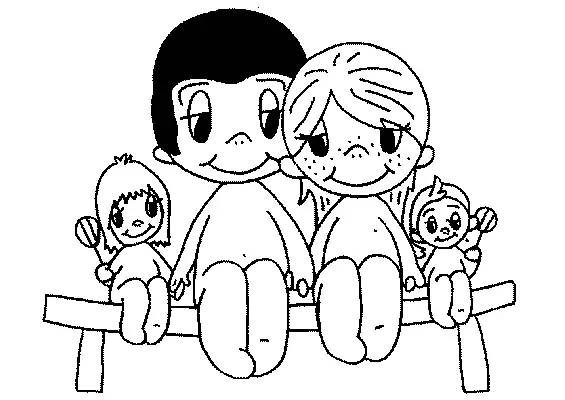
\includegraphics[width=0.3\linewidth]{images/xiaoyu2} 

}

\end{figure}

在鼓浪屿,京生特别依赖小语。小语走到哪里,他就跟到哪里;小语做什么动作,他就学着做什么动作;小语让京生做什么,京生就照做。只要小语走得远了,京生就大叫:``小语你等等我呀!''后来累了,只要小语在视野范围内,京生就安然无事,否则就开始哭嚎。

晚上回到宾馆,两人一起玩托马斯拼图。拼图上标着适合四岁以上儿童,因此超过四岁的小语拼得很快,不到四岁的京生用崇拜眼光地在旁边看,然后说:``小语你拼得真好呀!''我从没听过京生的语气有这么温柔。

回到北京,小语妈邀请我们去家里聚会。小语摆出了很多小火车模型等待京生来,两人玩得高兴,所以我们大人可以好好吃饭聊天。孩子还是有个伴儿好,省了大人多少心。

走出小语家之后,京生跟我说:``爸爸,我和小语玩得真好呀。''

快乐的时光总是短暂的。假期结束,京生又回到了德国。

\emph{3}

长久不联系,我以为京生又把小语给忘了。直到京生5岁的一天。

那一天,京生玩赛车玩具,突然大喊:``爸爸,妈妈,我和小语都赢了!''他说,这四台车里,小语开的是闪电麦昆。

我:``你怎么突然想起小语来了?''

京生:``因为小语是我姐姐。''

我:``你记错了吧,你说的是你表姐佳霖吧。''

京生斩钉截铁地说:``不,就是小语!''

我追问:"你怎么突然想起小语来了?"

京生:"因为我觉得搬家之前住的地方挺好看的。我觉得小语也挺好看的。"

再追问搬家之前是什么地方,京生解释:"就是我和小语一起玩沙子的地方。"

原来近些年京生住过的地方太多,错把3岁时厦门旅游那次记成了自己家。不知道这两天怎么突然想起了这事儿。

但是,你夸人家姑娘漂亮时干嘛这么严肃,难道不能象征性地羞涩一点吗?

又有一次,京生做噩梦惊醒,说是梦见地震了,弄得全家后半夜都没睡好。第二天睡觉前,自言自语说:"我不想做噩梦了。我想做美梦。"

妈妈问:啥是美梦?

京生说:"见到小语。"

后来又补充:"是没有变成怪物的小语。"

两天后,我问京生前晚做梦了没有。

京生:"做了。是好梦。梦见我坐上大汽车去幼儿园,遇见了小语。小语在画画。我说我小时候摔了一跤都没有哭。小语就这样式儿的(做拍手状),说真棒!"

我叹到:"你怎么最近天天想着小语?"

京生说:"因为小语挺好看的。因为我喜欢小语。一直喜欢小语。"

我再叹:"你真勇敢。"

京生说:"对,我是勇敢先生。''

勇敢先生出自《奇先生妙小姐》,是小语妈送给京生的一套画册。

我暗想:要是老子我从小就像你小子一样读勇敢先生,估计就不会见了女孩就一副怂样,当然今天就不是这个样子了。有诗为证:

\begin{quote}
沉舟侧畔千帆过, 雏凤清于老凤声。 长江后浪推前浪, 青出于蓝胜于蓝。
\end{quote}

\chapter*{数数}\label{counting}
\addcontentsline{toc}{chapter}{数数}

据说有一道幼升小的填空题是这样的:

\begin{verbatim}
(), (), (), 2, 4, 6, 7, 8
\end{verbatim}

这道题老爹我说什么也做不出来,但一看标准答案我就懂了:

\begin{verbatim}
(门前大桥下),  (游过一群鸭), (快来快来数一数), 2, 4, 6, 7, 8
\end{verbatim}

原来这不是数学题,而是音乐题啊。这是儿歌《数鸭子》的歌词。坑的就是爹呀。

这首歌旋律优美,节奏明快,正因如此,我非常讨厌它:小孩学得太快了,纠正都纠正不过来。3呢?5呢?为什么歌词不能写成4,5,6,7,8?照样押韵啊。

德生2岁的时候,开始自发学数数。他数数是这样的:

1,2,5,7,8,9,10.

不知道从哪里学来的。

回忆起京生2岁时,会一边上台阶一边自己数数:``1,2,3,4,5,6,7,8,9,10,11\ldots{}\ldots{}''后面数不清了。我们第一次听到的时候大吃一惊。因为此前京生只会从5倒数,或者正着数到6。不知什么时候起自己已经学会数到两位数了。

数数在孩子眼里,不只是表示``数数''。

有一次,我听京生说:``路!''

于是我问:``什么路啊?''

京生解释:``上路!''

我迟疑了,表示没听懂。

京生看看我,想找到一个方法给我解释。京生说:``1,2,3,4\ldots{}\ldots{}''

我恍然大悟。京生说的是``楼''、``上楼''。每次上楼梯的时候我都带着他数数。他用这种方式向我解释,这个思路有意思。

京生看我听懂了,很高兴地开始自己数数:``1,2,3,4,5,6,7,8,9,10,11,12,13,15,16,18,19,20!''

我惊讶地大叫京生妈:``你听见没?儿子数到20了!''

作为理科博士的京生妈一边做饭一边说:``听见了,就是少了14和17。''

奇妙的是,京生的这种诠释方法,似乎是儿童脑子里自然而然形成的,因为德生也是这样。德生指着台阶说:``1,2,5,7,8,9,10.''于是我便知道他想上台阶。

姥姥和姥爷来跟我们团聚,开始教德生数数。很快,2岁多的德生能把1到10数全了。这已经超过德国幼升小的要求了,幼升小只要求从1数到6。

前几天,德生竟然从1数到了40。可以直接上四年级了吧?

\chapter*{谨慎的孩子}\label{careful-boys}
\addcontentsline{toc}{chapter}{谨慎的孩子}

京生刚满2岁的时候,开始学着双脚跳。当然,那个时候还不能成功,只是象征性地向上用力。这样持续了四个月,京生一直在主动学习和练习双脚跳,最后终于完全学会了。2岁半的时候,他能双脚离地连续在原地跳十几下,能够向前跳三四十厘米,并且能够从台阶上双脚跳下来。他还试图跳上台阶去,自己做了几次向上的动作,大概是估摸着不太有把握,于是要求拉他跳上去。从这个小动作可以看出,京生虽然爱动,但却是个谨慎的孩子,不爱弄险。

谨慎的另外一个表现是玩滑梯。一米五高的滑梯,阶梯状的梯子,2岁的京生可以自己爬上去,滑下来,没有问题。当时,我家楼下有个两米高的滑梯,竖直的梯子,爬不上去,我把他扔上去,他坐在滑梯上,要求我站在着地的地方接着。

滑了两次之后,再次坐在那里,京生迟疑了片刻,对我说:

``太大。''

然后站起来,不滑了,要求我抱下来。

如今德生也2岁半了,也学会了双脚跳,只是还不会像哥哥那样往前跳那么远。玩滑梯的时候,比哥哥更小心。

这小哥俩从小就能够对要做的事情的风险进行评估后再行动,是让人放心的孩子。德生的表现跟京生当年如此相似,大概谨慎的性格是写在基因里的罢。

\chapter*{让孩子爱上喝水}\label{water-drinking}
\addcontentsline{toc}{chapter}{让孩子爱上喝水}

京生小时候,在奶奶家住过一段时间。奶奶经常跟邻居的老人们在楼下的院子里一起带各自的孩子。爷爷奶奶发现京生有个好习惯,好奇地问:

``你们是怎么让孩子爱上喝水的?''

这是京生的一大优点:爱喝水,白开水。

京生有个专门喝水的奶瓶,里面一般总是有水。经常看见的场景是,京生在屋里跑来跑去,跑到茶几旁边,拿起奶瓶就开始喝,咕咚咕咚喝光,停下来,举起奶瓶自己看看,说:``没有。''然后递给我们让给他加水。

这个举动让邻居的爷爷奶奶纷纷羡慕不已,因为他们的孩子不爱喝水,哄也不喝,而我们那儿的一般观念是,小孩火气大,喝水败火。

京生一下就成了榜样。

京生很喜欢他的喝水奶瓶。我和朋友一起吃饭时,京生坐在我们身边,每人面前一个酒杯。起初我还怕京生抢我们的酒,后来发现京生面前放他的奶瓶就行了,我们举酒杯,京生举奶瓶,一起碰,京生使劲往前探身,说:``干杯!''又是咕咚咕咚喝一大口,然后使劲放在桌子上。不跟他碰杯的话是不行的。

如今,德生也爱喝水。1岁多的时候,德生喜欢上一种吸管杯,带两个把手,握持很方便;有个盖子,很容易打开和关上。德生常常抓起吸管杯,咕咚咕咚喝完,然后塞到我手里,说:``加水!''

让这两个孩子爱上喝水的秘诀是什么呢?

\begin{enumerate}
\def\labelenumi{\arabic{enumi}.}
\item
  最重要的是,父母要爱喝水,孩子自然会跟着学。
\item
  要用孩子喜欢的瓶子或杯子,放在他们随手能拿到的地方。
\item
  当然,水要清洁,不要有让孩子讨厌的异味。
\end{enumerate}

\chapter*{出生在北京}\label{born-in-beijing}
\addcontentsline{toc}{chapter}{出生在北京}

\emph{1}

早就听说这个时代的中国生养个孩子是多么不易。京生出生之前,我们做足了思想准备。没想到,最初还是小小被打击了一下。

打击我们的是安贞医院。这家医院以治疗心血管病而闻名。选择它,是因为离家近,图个方便。

在一次常规检查后,我们问医生(或者是护士)情况怎么样。

我们期待的回答当然是``健康'',加上``非常''两字更好,最好语气加上一些兴奋。即使这样有些困难,那么平淡的语气也可以接受。如果是有什么问题的话,我们希望听到的是安慰。

结果,我们听到的回答是两个字:

``活的。''

我简直不相信自己的耳朵。尽管谁都不能否认这是个好消息,但我们觉得寒气逼人。孕妇心里觉得不高兴。于是,我们决定:

转院。

\emph{2}

转院,海淀妇产医院我们根本不考虑。我们转到了名不见经传的复兴医院。

这家医院据说原来只是个社区保健性质的医院,后来才发展起来的。有一次我打车去,司机很奇怪地问:``你们怎么选了这么家医院?我都找不着路。''

选择这家医院的直接原因,是因为产妇少。人少的话,大夫就顾得过来,就会有人性。这是老婆大人的意见。

事实证明,这是个英明无比的决定。

复兴医院比较特别的地方是门诊部和住院部是分开的,分别在月坛北街和木樨地地铁站附近,以至于头一次去我走错了地方。好在都不算太远。有时候老婆一个人去,有时候我陪着,产前的几个月我都记不得发生过什么了,这说明比较顺利,大夫的态度不像安贞那样让人刻骨铭心。

预产期到了。2007年的某个凌晨,大概一点钟,外面下着秋雨,感觉有状况了,岳母在家收拾东西,我出门叫出租车。我家附近有一处出租车集散地,我早就在打他们的主意了。很顺利打到车,直奔住院部。

\emph{3}

在医院的过程,我已经记不清了,只记得早早就把老婆推进了产房,而岳母和我在外面等待。一般都说此刻的感觉是什么焦急、期待之类的,而我主要是觉得困,然后就是一种很复杂的混合的感觉,说不清道不明。关键是当时比较忙乱,没工夫去把这种感觉梳理清楚。

据说产妇病床特别紧俏,价格昂贵,大概一天三百吧,我们决定试一试。我们找到值班护士,使劲儿央求,小护士看起来像个实习生,弄得有点手足无措。岳母偷偷给她塞钱,吓得小护士赶紧推开,答应看看再说。终于,我们争取到了一个独立的病房,两张床。行贿不成,在出院的时候,我用这笔款子买了一篮子水果,给医生姐姐护士妹妹们送了过去,表示感谢。

这的确是发自内心的感谢。感谢的理由有很多。

首先是京生很健康,这是最重要的。

跟我一起在产房外面等待的另外一个爸爸和奶奶,医生出来告诉他必须用产钳,产钳可能的不良后果如何如何,需要在免责书上签字。这个爸爸吓得脸刷地白了。当然得签字,没别的选择,必须走的程序,好在生下来的孩子也健康。当时我就想,什么男孩女孩胖了瘦了都无所有,只要健康。其实老婆早就知道是个男孩了,就是一直没有告诉我,把悬念给我留到了最后。京生出生一天后,医生特意跑来告诉我们,京生舌头下面有一点什么粘连什么的,建议给弄开,不花钱,很容易的根本算不上手术的一个小操作,不然可能将来影响说法吐字。京生姥姥说,这要是搁在别的地方,有毛病就有毛病,谁管你这么多。这个医院是真正为产妇和新生儿的健康负责的。

感谢的第二个原因是,没有被强迫剖腹。

据说顺产的产妇不多,据说医院都有指标,每年必须保证百分之几的产妇是顺产,完成任务后就可以随便切西瓜了。这都是据说,是真的吗?我不知道。

我知道的是,剖腹产对医院是有好处的:

第一是安全,医生操作起来不像顺产那么麻烦;

第二是赚钱,剖腹产的手术费用和产后恢复的开销大概是顺产的两倍。

对我们来说,如果有选择的话,我们当然选择顺产,因为剖腹产恢复得慢,谁被像切西瓜一样切上一刀都是活受罪,顺产的都去割麦子了而剖腹产的可能还下不了床。还有其他的坏处,比如容易得一些后遗症等等。花钱也多。

剖腹产对孩子的坏处是短期看不出来的。据说,在顺产的过程中产妇体内会产生一种物质输送给孩子,能大大提高新生儿的免疫力。据说,在顺产的过程中新生儿的头部被挤压按摩,对大脑发育有很大的好处。在胎位正常、产妇身体状况正常的情况下,有良知的医生会用顺产的好处鼓励产妇,想赚钱的医生可能会用剖腹产的好处来吓唬产妇。

所幸,我们遇到了一位好医生。当时还有一位产妇和我老婆在同一个产房------这也是为什么没有让我进去陪同的原因------在医生的鼓励下,两个新妈妈都成功顺产。

我为没能陪同分娩略感遗憾。不过,几年之后,德生在德国出生,我全程陪同,并且亲手用剪刀剪断了脐带。

\emph{4}

话说当时是中午,我正站在产房门口看当天的北京青年报,同时吃着方便面。此前托护士带进去了吃的喝的,就不见动静,不知道还要等多久。正在吃着,只见产房门缓缓打开,一位护士推着一个小车出来,问:``谁是**的家属?''我说我就是。她说:``生了!''我一惊,扔下报纸和方便面就跑了过去。后来老婆说这可以作为一个广告创意,广告词叫做:

``惊喜时刻,康师傅与您同在。''

我吃惊主要是因为什么动静也没听见。看电视电影里,产妇总是在撕心裂肺地惨叫,医生总是在大喊``使劲'',男人总是在门外团团转。而我却在平静地吃方便面。老婆呢?老婆后来告诉我,她和同屋另一个产妇商量了一下,为了节省体力,没喊。

我跑过去,围着小车。襁褓里的小家伙睁大眼睛看着我,安安静静。我把右手食指伸向他的右手,他轻轻地握住。

这让我想起Friends里的那一幕。

这一握,把生活的书本翻到了新的篇章。

\chapter*{出生一个月}\label{one-month-young}
\addcontentsline{toc}{chapter}{出生一个月}

作为新生儿的京生个子长得飞快,表情也丰富起来,会注视,会好奇,会皱眉头,会哭,忘了这个时候会不会笑。哭的时候居多,以至于我做了一张``京生九天''的录像光盘给京生的曾外祖母看,老太太看了直说:快哄哄他,别让他再哭了。

说说京生出生后一个月的感受。

首先,我要感谢国家和感谢领导。国家规定,我所在工作单位的新爸爸有半个月的陪产假。但是,我工作的部门非常忙,加上接近年底,人手短缺。我请示领导,这假我休不休?

领导大手一挥:休!然后给我讲了一番道理:

不光要休,还一定要在家伺候着,否则日后夫妻吵架,女方就总会拿这个说事儿,男人就会理亏,那可是男人一辈子的思想包袱。这个包袱咱不能背啊!

于是,我结结实实过了一把``伺候月子''的瘾。

月子的日子很难过。我家三十多平米的使用面积,住我们夫妻俩正合适,现在成了三口之家,有点紧张。加上京生的姥爷姥姥过来照顾,空间已经严重不足。可是,竟然还请了个月嫂住在家里!

这是暗无天日的一个月。每天,门窗都关得紧紧的,说是怕``风''。看见抖一下窗帘空气动了一下都紧张。其实,中医的``风''不是空气流动的wind,但是,在这个时候,做科普是徒劳的。而且还怕光,窗帘也总是拉上。我只能安慰自己,京生幸好不是生在夏天。

然而,最大的惊奇是,我突然发现,自己从小就是一个家庭的中心人物,结婚后再怎么说也算是半边天,而此刻算是画上了句号。这个家的重心,已经永远地转移到了产妇和新生儿的身上,而新爸爸是没人搭理的。

我最不爽的是这个月嫂,嘴巴很甜,让我们一直有种错觉,觉得这个月嫂不错。后来我发现,大概是这个月嫂已经不算年轻,手脚不太勤快。京生妈因为比较辛苦,半夜京生哇哇大哭的时候她醒不过来,而经常需要我起来抱着哄,喂奶。回头想想,当时月嫂干什么去了?满月的时候,京生妈跟我商量是不是让月嫂继续做一个月,我坚持否决了。其实我知道,从一开始,月嫂在这里只是给大家尤其是京生妈一个心里安慰而已,从男人实用主义的角度说,没用。月子里那点儿活儿根本用不着这么多人手,合理安排一下,情况原本可以改善很多。

但是,这个时候,让女人安心,却成了最大的实用主义。你说应该通风透气,保持空气新鲜;你说应该拉开窗帘,才有利于新生儿视觉发育;你说月嫂没用,有父母照顾足够了。但是,女人不同意,有什么办法呢?这个时候女人说了算。永远不要在这个时候跟女人较劲。作为男人,随女人去吧,紧紧捏住忍字诀,天塌不下来。

而且,看着京生一天一天长得飞快,又有什么不能忍呢。

\chapter*{三岁分水岭}\label{three-year-young}
\addcontentsline{toc}{chapter}{三岁分水岭}

三岁是个分水岭。台湾作家汪培珽写过一篇文章,《二胎,用3年换未来30年》,其中的``3年''指的就是这个意思。养娃主要是前三年辛苦。等娃过了三岁,大人就省心了。

确实如此。

\textbf{数学}

三岁的京生,数数能流利的从1数到29。经常在30转不过弯儿,被提示后可以继续数下去。

京生会手指加法。比如我问``2加3等于几'',京生一只手伸出2个手指,稳住不动,另一只手伸出3个手指,两手并在一起,开始数:``1,2,3,4,5。等于5!''

京生我看了他的作业本,整页整页的数字,还有幼儿园阿姨打的对勾。

\textbf{逻辑}

京生已经完全理解了逻辑上的因果关系。表现为经常用``为什么''提问,自己也会用``因为''来回答大人的问题。

我家卧室临街,晚上窗外车声不断。有一次睡觉前京生透过窗户前往外看,问:``爸爸,汽车为什么不回家睡觉?''我说:``有的汽车在上夜班,晚上工作,白天才回家睡觉。''第二次京生又问了同样的问题,我仍然这么解释。京生就不再问了。后来我听到京生跟奶奶解释:``汽车在上夜班,晚上不睡觉。''

京生喜欢跑,跑得很快,所以上街我总是死死拉着他的手。奶奶同时拉住他另一只手的时候,京生就像其他所有的小孩一样,喜欢双脚离地打秋千,弄得大人很累,而且走得很慢。大人让他``好好走路'',但是不灵。于是我想了个办法。

我说:``你只能拉一个人,是拉爸爸还是拉奶奶?''

京生想想说:``拉爸爸。''于是就松开了奶奶的手,好好走路了。

从此以后,哪怕是京生本来拉着奶奶,我只要一拉住他的另一只手,他立刻就松开奶奶的手,说要``拉爸爸''。他明白了在一种逻辑下做出自己的选择。

有一次,我对京生解释:``爸爸拉着你是因为周围汽车很多,你自己走的话怕被撞着。''后来有一次过天桥,京生问:``爸爸,我可以自己走吗?''

我问:``为什么?''

京生说:``因为桥上没有车。''

我说:``可以。''

京生就高兴地松开我的手,跑上了桥。

京生最喜欢睡前看动画片《爱探险的朵拉》,原来喜欢的托马斯和米老鼠都退出了舞台。京生对朵拉如此着迷,有时睡觉之前看完一集还想看,就会小声说``再看一集''。满足他的要求再看一集后,就乖乖地上床睡觉了。京生是个讲道理的孩子。如果前一晚没看就睡了,第二天早上他会说:``爸爸,我想看朵拉。因为昨天晚上我没看。''

京生有时会利用他的讲道理这个优点来耍一些小聪明。因为他的牙不好,我会限制他吃甜食。有一次京生想吃奥利奥,我不让。京生可怜巴巴地就问姥姥,得到许可后就吃起来,被我看见质问,京生说:``是姥姥让我吃的。''把责任推得干干净净。

我竟然无法反驳他,于是有些担心。等京生长大了,我可能镇不住他。

\textbf{语言}

京生可以区分同义词。有一次忘了发生了什么事情,小语说:``我有一个好办法。''

京生看了看小语,跟着说:``我有一个好主意。''

京生妈是东北人,东北话里``主意''比``办法''常见。这至少说明三点:京生知道这两个是同义词;京生倾向于用自己熟悉的语言来表达同样的意思:京生喜欢与众不同。

有一天,我拉着京生在小区里走,京生说:``我们不走马路,走人行道。''

我说:``人行道上有树荫,好凉快。''

京生说:``对,树荫把人行道挡住了。''

我纠正:``不是树荫人行道挡住了,是大树把太阳挡住了,在人行道上形成了树荫。''

京生说:``对。你真聪明。''

我一时精神错乱,弄不清到底谁是大人谁是小孩。只好说:``你也聪明。''

想不到京生又来了句总结:``对,我们两个都聪明。''

真能说。

有一天,京生从外面把姥姥关在了洗手间里。我们要出门,可京生就不让姥姥出来。最后我佯装生气了,京生看着我的脸色,把洗手间门打开,说:``姥姥,我是跟你玩儿呢。爸爸,我是跟姥姥玩儿呢。''

京生跟电视里的朵拉学会了英文数数。京生说:``one,two,three,four,sit!''不仅漏了5,而且把6念错了,十分可爱。

京生有一次回到姥姥家,给我打来长途电话。我一接,京生就说:``爸爸,我回到姥姥家了。小舅接我,我去小妹家玩了。''发音标准,语句流利,把我吓了一跳,我还以为是京生的表姐冒充京生打给我的呢。

\textbf{生活常识}

京生学到的生活常识,主要体现在出行上。

大概是从小京生就被我们带着四处奔波的缘故,他有了很多交通方面的经验。比如说,一上车或上飞机就自己找安全带。坐机场大巴的时候,四处找不到安全带,我只好跟他解释,这辆车没有安全带,所以坐稳扶好就可以了。

有一次我们上了机场大巴,人比较少,京生坐在我旁边的座位上。后来上的人多了,我就把京生抱在我腿上,给一位老太太让座位。中途前排有人下车,空出了个座位。一直没吭声的京生看看旁边的老太太,指指前排的空座,说:``那儿有座位。''老太太笑着说这孩子有意思,想让别人离开也不直说。

有几次坐公交车和地铁,一有座位就让京生先坐下。再发现有空座位,京生就用全车厢人都听得到的大嗓门喊:``爸爸,这里有座位!''

京生对红绿灯的概念更加清晰了,自己会说``红灯停,绿灯行''。每次过马路的时候,我都不失时机地重复给他讲红绿灯的用途。这样的结果就是,如果大人图省事,闯红灯过马路时,京生就会毫不留情的指出:``你做得不对,不能闯红灯。''

观察了好几年,京生都严格遵守交通规则,于是在7岁上小学时,我们可以放心地让他自己上学。

\textbf{体能}

京生是个超标儿童。三岁七个月的时候,1.1米的身高,40斤的体重。他的饭量甚至超过了奶奶。

超标儿童的好处是体力很棒,从而内心比较彪悍。京生一般是不会主动要求让大人抱的。在厦门旅游时,我们从理工学院穿过厦门大学一直步行到白城海滩,对一个孩子来说相当远了。走累的时候,京生会蹲下来,说:``京生累了。''过一会儿接着走,不用抱。

京生经常主动要求做一些事情,比如说,看见我拖着拉杆箱,他也要拖,从超市一直拖到家门口。再比如,我们去看望刚生了孩子的老同学,我买了两大袋大约60片装的纸尿裤,我拎着都觉得沉,京生居然帮我拎着走了一段路。

当然,也有凄惨的时候。那时,京生看见小语做什么他就做什么。当体重不足30斤的小语被抱着的时候,京生也要求抱,我只有欲哭无泪了。

\textbf{音乐}

京生刚会坐的时候,就会跟着吉他的节奏摇摆。2岁的时候i,京生能够区分不同的歌曲旋律了。他当时要求听``汽车音乐'',就是动画片Cars的插曲
Real
gone。其他的歌曲,哪怕是同一影片中同一风格的,京生都能听出来不对,要求换回来。京生能唱大概10首儿歌。听到我在电脑里放李斯特的钢琴曲,京生能听出这是他会唱的《小星星》,这说明他的确是根据旋律判断,而非歌词。

晚饭后我们去小区公园散步,京生唱起他最喜欢的《两只老虎》,我跟着他吹起了口哨。唱完后,我说:``京生你唱得真好。''京生很对仗地说:``爸爸你吹得真好。''以后每次散步唱歌,都要求我吹口哨,并且要``123开始''一起来。

后来,京生从6岁开始学钢琴,一直学到现在,对音乐的兴趣从未中断。

\textbf{性格}

京生是个操心的孩子。在机场托运行李,京生歪着脑袋眼睛一眨不眨地看着我们的箱子被传送带运走了,等我办完手续,京生问:``爸爸,我们的箱子去哪儿了?''等上了飞机,我把随身的书包放进行李架,京生在座位上只看见我举起书包然后书包就不见了,就很关心地问:``爸爸,我们的书包去哪儿了?''

京生很大方,懂得分享,经常把手里的食物分给家人和小朋友吃。我带着京生在超市买了一盒12只装的可爱多冰淇淋,京生拿出来一个香草味的,我拿出一个巧克力味儿的,我们俩一边吃一边往家走。

我说:``京生,回家给大家发冰淇淋吃好不好?''

京生说:``好。给姥姥和奶奶吃香草味儿的,给姥爷吃巧克力味儿的。''

两个口味的冰淇淋外观不同。到了家,京生分发,一点没错。冰淇淋是很小的迷你型,我原以为京生会借机再吃一个,可是他没有,看着别人吃他一点也不眼馋。

朵拉里有个透着邪气的小狐狸叫捣蛋鬼,是给朵拉添麻烦的,每次京生都能预感到他的出现,------不知道是根据记忆,还是根据剧情,或者是根据音乐,------然后就害怕地躲在大人或被子或椅子后面,或者躲在房间某个角落,直到捣蛋鬼被赶走。

有一次我跟京生说:``京生,你跟朵拉一起说``捣蛋鬼,别捣蛋''就可以了。捣蛋鬼就被赶走了。''京生就听话地跟着说。

从此,京生再也不躲了,每次都很紧张地跟朵拉一起把捣蛋鬼赶走。

京生奶奶说,我有时候对京生太严厉了,京生有点怕我,有时候会看我的脸色。也许吧,这未必是坏事。京生并没有因此而疏远我。相反,有原则的成年人让孩子更容易有安全感。

有一次京生要求看书,可是没带书来北京。我就翻出一本``不可忽视的真相''给他看,里面有很多地理气象类的图片。京生看见后兴奋地说:``我要看地图!''于是翻到世界地图那一页。不管他懂不懂,我给他讲北京在哪里,姥姥家在哪里,妈妈在哪里。

我问:``你是喜欢和爸爸妈妈在一起呢,还是喜欢和姥姥姥爷在一起?''

京生说:``我喜欢和爸爸妈妈在一起。''

我问:``为什么呢?你在姥姥家不是玩得挺好吗?''

京生温柔地说:``我就是喜欢嘛!''

喜欢,不需要理由。喜欢就是最基本的理由。

就这样,过了三岁,似乎是突然之间,京生就有了自己的思想,并且想法越来越多,给大人带来更多的乐趣。京生再也不是一两岁的小孩了。

如今德生两岁多。日子过得手忙脚乱的时候,我就数着德生的年龄,心想,快了快了,苦尽甘来的日子不远了。

\chapter*{三国分居}\label{three-kingdoms}
\addcontentsline{toc}{chapter}{三国分居}

来德国读博士没多久,我被派到韩国做野外观测,京生妈在德国忙着做实验,实在照顾不过来,就把京生送回了中国。一家三口,三国分居的日子开始了。

京生先是在姥姥家住过一段时间,后来又住在奶奶家。

在奶奶家,除了没有电脑可以和爸爸妈妈视频,除了没有电脑看闪电麦昆之外,没有任何明显的不适应。看来给奶奶家买个电脑装上互联网是势在必行的事了。

没有了视频聊天,京生学会了接电话。每次打过去电话,都是京生抢着接的,就听见耳边小朋友的声音:``你是谁?''

我:``我是爸爸。''

京生直来直去,从来不会客气:``你找谁?''

我:``我找你呀。''

京生:``你为什么找我呀?''

我说``我想你了'',然后就问京生在干什么,吃饭了没有,去幼儿园了没有,然后我就不知道该说什么。不在一起生活,我跟一个四岁的孩子没话题啊。

我说:''京生把电话给奶奶吧,爸爸想跟奶奶说话。``

京生不干:``不嘛,我要跟你说话!''然后沉默。

他跟我一样,也不知道该说啥,但是还想说。于是,京生开始胡说,想起什么说什么,包括不知从哪里学来的骂人的话,比如``你是一个臭小子''之类的。说完就笑。

我想,骂就骂吧,新学来的东西,肯定是好奇,多练练也好,将来纠正也不迟。这孩子想跟爸妈多聊天,却不知道该说啥,难为他了。

说了一会儿就走上正轨了。京生给我背了好多新歌谣,我都没有听过。

虽然奶奶不懂英文,京生却喜欢跟电视自学。有一回,京生嘴里突然蹦出了很多呜哩哇啦的词语,我们一时没反应过来。重复一遍,我听懂了,是很多水果的英文名称,比如apple,orange之类的,发音挺标准的。

京生还学会了英文的生日歌。有一次幼儿园阿姨让京生上台表演,放学的时候阿姨对京生奶奶说:``今天京生给大家唱了一首德语歌。''估计是歌词谁都没听懂,阿姨就误以为是德语。

京生狂热地自学外语,这个不是一般小朋友能有的爱好。为什么会这样呢?

我们分析,估计是京生两岁多刚开口学说话的时候,正值在德国上幼儿园,环境给了他潜移默化的影响,当时想说说不出来,憋着了,印象里种下了外语的种子。现在,语言能力突飞猛进,这颗种子被激活了,虽然身边没人教,但是有朵拉一类的动画片给浇水,苗儿就疯长。

有一次我问:``京生你喜欢住在奶奶家还是姥姥家?''

京生说:``我喜欢住在姥姥家。''这个有道理。姥姥家有电脑,有表姐表妹一起玩,有山有水还有班长可以当。

然后京生说:``姥姥病了要看牙,所以我住在奶奶家。''

我们怕京生误以为姥姥不要他了,就给他的解释是姥姥要看牙,没时间照顾他,看好了牙再来接他。

这个理由很管用,一是不用把姥姥的身体状态解释过于复杂,二是趁机教育京生勤漱口刷牙。

多少次的较量证明了,对京生粗暴地硬来是不行的。京生的特点是吃软不吃硬,好声好气跟他讲道理,他就能接受。

京生在幼儿园上中班,这属于复读,他在姥姥家就是上的中班。京生自己解释:``我长小的时候上小班,长中了上中班,长大了上大班。''

我最常问京生的问题之一是,在幼儿园玩啥了。有一次京生突然说:``我和小语去看大海了,我们没有去海里游泳。''嗯,小家伙难道是在做梦?我暗想,儿子,还想着小语呢,你大概不知道,小语身边已经有个姓王的小子了吧。

往常京生说完话,用不挂电话这种方式表达对爸爸妈妈的思念。今天,京生说:``爸爸,我想你。妈妈,我也想你。我想找爸爸妈妈。''

我心里一酸,一下没忍住。

\chapter*{好想回到小时候}\label{if-younger}
\addcontentsline{toc}{chapter}{好想回到小时候}

京生四岁时,曾经说他喜欢小小智慧树的红果果和绿泡泡。我不认识,就问是谁。京生说:

``红果果是个美丽的女人,绿泡泡是个帅气的男人。''

京生妈妈问:``那你更喜欢哪一个呢?''

京生说:``我更喜欢绿泡泡,因为男孩应该跟男孩玩。''

京生妈妈私下狠狠地说,京生喜欢的应该是女孩!

京生继续说:``爸爸,我想要个哥哥。''

我和京生妈讨论了一下,觉得这个难度有点大,就问:``你为什么想要个哥哥呢?''

京生说:``杨蕾就有个姐姐。''

我问:``杨蕾是谁啊?''

京生用跟刚才一样的口气说:``杨蕾是个美丽的小女孩。''

原来杨蕾是京生幼儿园的同学。京生觉得女孩有个姐姐,那么男孩就应该有个哥哥。

据说定期扔东西可以提高生活品质。我们翻出了一些旧物,其中包括京生2岁时用过的椅子。这椅子京生已经两年没见过了。

京生问:``这是什么呀,爸爸?''

我说:``这是你小时候坐过的椅子。还记得吗?''

满以为京生会说``记得''或``忘了'',不料京生说了一句:

``我好想回到小时候啊!''

说这话的京生年纪是四岁半。

我暗想:谁不想回到小时候啊!

\chapter*{性别意识与婚恋观}\label{sex-edu}
\addcontentsline{toc}{chapter}{性别意识与婚恋观}

京生四五岁时,已经知道了小孩是从哪里来的,知道了男女有别,并且初步有了自己的婚恋观。

拜罗伊特市郊有片森林,森林的池塘边有配图的文字,展示蝌蚪如何变成青蛙,青蛙又如何生出小蝌蚪的。这是对儿童进行性教育的好机会。我给京生讲解完青蛙后发挥了一下,说:

``人也一样,你看爸爸以前也是小孩,长大了结婚后生了你。你以后也会长大结婚再生个宝宝,也会当上爸爸。''

京生问:``那宝宝会在我肚子里吗?''

我说:``不会,你结婚娶个老婆,宝宝会在你老婆肚子里。你想要个什么样的?''

京生说:``我想要个长头发的,就像玛丽娜那样的,因为我喜欢女孩。''

我:``我问的是你想要什么样的老婆,不是什么样的小孩。''

京生说:``我想娶个海蒂那样的老婆。''海蒂是京生所在的幼儿园彩虹班三大美女之一。

我说,那你得对海蒂这样的小女孩好一点,不要跟她抢玩具,有好吃的要分给她。

京生想了想说:``那我还是娶艾薇莉吧。''艾薇莉是邻居家的小姐姐,11岁了,经常领着京生在楼下公园玩,照顾他。

我问为什么。京生说:``艾薇莉长大了,不会抢我的玩具。''

我说,她比你大六岁!

京生说:``我长到爸爸这么大的时候再娶她!''

有一段时间,京生从动画片里学会了向星星许愿。德国冬天天黑得早。有一次,从幼儿园回家的路上,满天星斗,地平线上方的猎户座颇为壮观。京生停下脚步,双手交叉胸前,虔诚仰望,嘴里念念有词:

``我想赶快长大,生个小宝宝。''

妈妈大惊,追问何故,京生解释说:``我已经是大孩子了,我不想只让别人觉得我可爱,我也想觉得小宝宝可爱。''

京生班里有个小男孩尼克,家里有几个姐姐。这个小男孩就学来了一些小女孩的表情、语言和动作。京生也受到了影响,有时候扭扭捏捏哭哭啼啼。我纠正:``不要再学小女孩了,也不要学尼克。难道你想变成个女孩吗?''

京生说:``不想!''然后发挥了一下:``我想当男孩,不想当女孩,因为女孩长大了生小孩的时候会肚子疼,我不想肚子疼。我在妈妈肚子里的时候就一直想当男孩,所以我生下来了就是男孩。''

原来京生是男孩的原因是他怕将来肚子疼。

京生:``我最喜欢逛超市买东西了。''

我:``你有钱买东西吗?''

京生:``我没钱。''

我:``那你怎么买东西?''

京生:``你给我买。因为你有钱。''

我:``我为什么要给你花钱买东西?''

京生:``因为你是我爸爸。''

我:``那等你有了钱,你也得给我花钱买东西,因为你是我儿子。''

京生说:``不行。等我有了钱,我还要花钱给我自己的小孩买东西。''

真是个好爸爸。

电视里放相声,京生正在卫生间方便,听见客厅电视里传来的笑声,问:``爸爸,为什么有人笑?''

爸爸:``两个人在说笑话呢。''

京生:``什么笑话?能不能说给我听听?''

爸爸:``是相声,大人听的,小孩听不懂。''

京生:``那你讲给我,我记下来,等我长大了我讲过我的小孩的妈妈听。''

真是个好老公。

\chapter*{绯闻女友薇拉}\label{vera}
\addcontentsline{toc}{chapter}{绯闻女友薇拉}

大概每一桩包办的背后,都有一个叛逆的故事,连五岁的京生和小语也不例外。

作为父母,我们自然尽量给他俩创造机会,不惜跨越万里的遥远距离安排一起度假。可是,天不遂人愿,小语有了个塌鼻子小男友,并数次拒绝了跟京生视频聊天;京生闷了几天,很快,也有了新的小伙伴。

京生刚来德国的时候,初进幼儿园,语言不通,生活的苦闷程度可想而知。可是很快有一天,京生回家来很高兴地说:``老鼠组有个会说中文的小朋友,他的名字叫萨-莫-耶!''

京生的幼儿园分三个组:瓢虫组,老鼠组,以及京生所在的彩虹组。各组有各组的文化氛围。比如,瓢虫组的吉祥物是只瓢虫,老鼠组的是只老鼠,彩虹组的------是只大公鸡。七彩尾巴的大公鸡。各组不分年龄段,混搭。小孩子们一天之内在幼儿园呆的时间不同,短的呆三四个小时,长的八九小时直到幼儿园下班。这样,下午的时候,有的已经被接走了,没被接走的孩子全部被划拉到一个组里交给两三个老师看管,老师们可以轮流提前下班。于是京生有机会接触不同的氛围,结识别组的小朋友。

萨莫耶,我们觉得奇怪:谁家给孩子取这么个名字?

后来去幼儿期了解了一下,这个男孩其实是叫Samuel,比京生大半岁。京生自己用汉字的发音去念他的名字。好吧,那就叫他萨莫耶。

萨莫耶的爸爸是俄国人,妈妈是台湾人,家里的官方语言是英语。真正的国际家庭!萨莫耶的母语是英语和國語。他不说俄语。萨莫耶还有个两岁多的妹妹,叫薇拉。

没过多久,薇拉也被送到了这个幼儿园,分到了京生的彩虹组。京生说:``薇拉天天哭。''

是的,第一个月,每天早上彩虹组里都有薇拉惊天动地的哭声。有一次我不忍心看,上前想哄一下,结果薇拉哭得更凶了。安老师说,别碰她。

第二个月的时候,薇拉就不哭了。

后来,倒是年纪小的薇拉经常把年纪大的京生弄哭。有时候是薇拉动手把京生打疼了,也有时候是心里委屈。

有一次,薇拉说京生是女生,京生说不是,薇拉说是,如此反复说了好多次。回家的路上,京生对我说:``我不喜欢薇拉说我是女孩。爸爸,我该怎么办啊?''

我说:``她还太小,不懂,你就让她说嘛,你又不疼。''这个答复显然让京生失望了,京生竟然失声痛哭起来。哄了很久才平静下来。

哭归哭,玩起来不记仇。京生和薇拉兄妹的关系越来越好。后来,两家大人带着孩子互相来家里作客。

薇拉妈妈看上去不大,却说自己是73年生的,后来才弄明白,是民国73年。我们发现,三个孩子在一起,比两两在一起复杂多了。任意两个之间都会因为抢玩具而打起来,打完就哭,哭完接着玩。有一次薇拉说:``我不是薇拉。''京生说:``你是薇拉。''薇拉说:``我不是。''京生说:``你是。''像回声一样重复了十几个回合。

此时萨莫耶一直一声不响地低头自己玩玩具,大概是听得不耐烦了,抬头对京生用冷冷的口气说:``别理她。''

薇拉拿着京生的麦昆扑克牌问,这个怎么玩。京生拍拍薇拉的脑袋,用大人的口气说:'你还太小,你不懂。'
薇拉说:'我已经长大了。'然后把手举得高高的。

在我家完了一天,薇拉兄妹要回家了。薇拉妈妈边穿外衣边说:``薇拉,快穿衣服,不穿的话你就在京生家别走了。''薇拉一动不动。薇拉妈妈说:``那,再见。''薇拉对妈妈招招手,说:``再见!''

虽说经常抢玩具,不过小朋友们也都很大方。京生5岁生日的时候,收到了薇拉家送的礼物:玩家直升飞机和汽车。这套玩具保存至今,现在归德生玩。

薇拉过三岁生日,京生画了个蛋糕,写上自己和薇拉的名字,贴在一本魔法小姐的书上送给了薇拉。京生还在过年的时候送给萨莫耶和薇拉每人一套乐高玩具,后来萨莫耶也回赠了京生一套有三种拼法的乐高玩具。赠送礼物成了习惯,于是就发生了下面的故事。

萨莫耶指着京生心爱的一套乐高玩具问京生:``可不可以送给我你这个玩具?''

京生为难地说:``不可以,这个我太喜欢了。要不送你别的东西吧。你想要什么?''

萨莫耶:``那可不可以送给我这把吉他?我可以送给我爸爸。''

京生:``可是这是我爸爸的吉他,不能送给你。要不,''京生指了指书桌前的椅子,``这把椅子送给你把,你可以给你爸爸坐。''

萨莫耶:``可是我家里有椅子了。''

京生:``那这双拖鞋送给你吧,可以给妈妈穿哦。''

萨莫耶:``我不要。''后来要离开时很忧郁的说:``我都没有礼物。''

京生从房间里拿出一个白色小汽车玩具,塞到萨莫耶手里,说:``这个送给你!''萨莫耶这才高高兴兴地出了门。

因为语言无障碍,薇拉成了京生的跟屁虫。京生也很乐意,甚至跟别的男孩争风吃醋。

薇拉吃饭的时候喜欢坐在京生旁边,同班的尼克拉斯很生气,因为他喜欢薇拉。有一次,京生和薇拉抢玩具,薇拉很不高兴,跟尼克拉斯吃饭去了,京生只得跟莉妮坐在一起。

京生说:``我不喜欢莉妮,她总是拉到纸尿裤里。我喜欢薇拉。''

当然,薇拉的生气很快就过去了,又会回到京生的身边,因此大多数情况下是尼克拉斯在旁边眼红。

每天早上,京生一到幼儿园,顾不上换衣服就找薇拉,找到后大声喊着薇拉的名字。薇拉大声表白:``京生!京生!我喜欢你!''京生也大声回应:``薇拉!我也喜欢你!''有一次薇拉说:``京生,我要保护你!''京生愣了一下,原样回复:``薇拉,我也保护你!''然后两个孩子拥抱。

为此,我有些担心,不知道薇拉的父母是否介意,就私下和京生谈了谈:

``京生,女孩子不能随便碰的,除了拉手,女孩子身上其他的地方都不能碰,明白没?以后不要抱薇拉了。更不能亲她。''

京生说:``可是薇拉要抱我,该怎么办啊?''

京生爸:``那你就让她抱,你是男孩,不吃亏。''

幼儿园的老师也发现了这一对儿的关系非同一般。安老师很神秘地跟我说:``他们两情相悦。''后来一天早上,京生一到幼儿园又大声喊薇拉的名字,安老师笑着大声说:

``Big love!''

\chapter*{动画片《雪孩子》的误导}\label{snow-kid}
\addcontentsline{toc}{chapter}{动画片《雪孩子》的误导}

小孩子没有哪个不喜欢看动画片。有些动画片貌似优秀,却未必完全适合孩子看,大人平时不注意的话,后果可能不堪设想。

京生小时候,有段时间喜欢突然挑出来大喊一声:

``呔!你这个大坏蛋!''

毫无疑问,这是从《葫芦兄弟》里学来的。我们讨论很多次,觉得其中的打打杀杀暴力元素太多,最后不让他看这个动画片了。

有一年冬天,京生缠着让我给他堆雪人。可是,那个冬天雪下得太少。于是我说:

``要不给你看个动画片吧,爸爸小时候非常喜欢的,叫做《雪孩子》。''

京生拍手赞成。

《雪孩子》是国产系列动画片《小兔淘淘的故事》中的一集,拍摄于1980年,画面精美,配乐动听,那两首插曲,``雪花,雪花\ldots{}\ldots{}''和``挥起小铁锹''的旋律,我时隔多年还能哼得出来。

然而,这次在Youtue上翻出来重温,却发现了故事里有两个严重问题,必须适时加以引导。

《雪孩子》的故事是这样的:兔妈妈去森林里找食物,留下小兔淘淘独自在家,临走前堆了个雪人陪淘淘。淘淘玩累了回家睡着了,但屋子里炉子跳出的火星燃起了大火,雪人奋不顾身冲进去把淘淘救了出来,自己却融化了。

多年来,我一直没有觉得哪里有什么不妥,直到有一次给京生读《365夜故事》里《雪孩子》的原著。

跟动画片的情节不同之处在于,原著故事的结尾增添了其他小动物的戏份:森林里其他的动物们帮忙把火扑灭了,但是太晚了,雪孩子已经融化了。正因为这一点点不同,我这才发觉是哪里出了问题。

思考片刻,我给京生详细解释了一下:

雪孩子热心救人,想法是好的,但舍己为人的做法是错的。因为他没有能力把淘淘从火里救出来。

京生说:``可是他把淘淘救出来了啊。''

我说:``但是他自己却死了。他有了生命,跟淘淘是一样的,不能为了救活淘淘就烧死了自己。你想想,有没有办法既能让雪孩子活着,又能把淘淘救出来?''

经过讨论,我们得到最后的答案是,去请其他动物过来帮忙救火。

我还不放心,再三嘱咐:``你千万不要学雪孩子。你是小孩,看见危险首先要躲开,保护好自己不受伤害。想帮助别人的话,找大人来帮忙,这样你仍然是个小英雄。''京生点头。

作为成年人,应该千方百计确保儿童的安全,而不是鼓励他们有什么牺牲精神,做什么小英雄。不仅是雪孩子,还有王二小、雨来、赖宁\ldots{}\ldots{}那些出于时代的特殊需要所塑造的小英雄形象,要么不讲,要么给孩子讲完之后增加个讨论环节,否则就是误导孩子。

然后,我和妈妈私下讨论了另一个问题:兔妈妈能把淘淘单独留在家里吗?这场大火,兔妈妈要承担多大责任?如果小兔被烧死烧伤,兔妈妈是不是应该被判刑?

为此,我搜索了一下,各国法律对此的规定有不同,但共通的一点是,如果孩子是因为身边没有大人而出了危险,显然是监护人的失职。希望《雪孩子》的结局能加上一段:猫头鹰爷爷批评兔妈妈,你怎么能把淘淘单独留在家里呢?

以前,我对上面这两个问题并不在意。来德国之后,我经历了两件小事。有一次,我在公园散步,突然跑过来两个五六岁的小孩,他们发现地上有个纸团在落叶里冒烟,于是并没有自己救火,而是在周围找大人,拉我到树丛里,把地上冒烟的烟头指给我看,让我帮忙灭火。

还有一次,我让京生一个人在公园的儿童乐园玩,我在周围跑步。离开没几分钟,我就被经过的不认识的德国人抓住问,那边有个单独玩的孩子是不是你的孩子?

误导儿童舍己为人,忽视监护人的失职,这就是我在动画片《雪孩子》里发现的两个问题。

话说回来,动画片的确拍得好看。京生对雪孩子念念不忘。后来,虽然过了个暖和的绿色圣诞节,
3
月份终于下了好几场大雪,我们一起堆了个大雪人,并且应京生的要求,在雪人身上写上``雪孩子''三个字。

妈妈说:从来没有堆过这么大的雪人!

\chapter*{学骑自行车}\label{bike}
\addcontentsline{toc}{chapter}{学骑自行车}

以行动的空间尺度来给人的一生划分阶段,是个有趣的视角。

1米:小孩从刚刚出生到一岁左右,他的行动空间局限在爸妈的怀抱、家里的摇篮、外出用的童车,距离大人的尺度一般在一米以内。

10米:一岁时学会走路,从迈出第一步到围着撒欢儿跑,行动尺度拓展到十米到数十米,这是成长的第一个里程碑。

100米:后来,他学会了使用一种交通工具,迎来了第二个里程碑,他终于突破了百米的行动尺度,父母只能远远地看着,内心既欣慰又担忧,不得不面临这样一个事实:当他在远处摔倒的瞬间,再也无法及时伸出扶他的手。

5岁时,京生学会了骑自行车。这件事上他打破了家里的记录,因为学会骑车的年龄,京生爸是16岁,京生妈是10岁。

京生身高超标。四岁时,大人自行车上的儿童座椅和京生自己的小拖车都已经坐不进去了。于是,我们在跳蚤市场买了一辆16寸的儿童自行车,两轮。这对京生是个挑战,因为他只骑过三个轮子或附有两个辅助小轮的自行车。试骑,骑不好,也许对于4岁多的孩子有点太难了。不得已,又买了两个辅助小轮安在后轮上。在确保不摔的前提下,京生天天骑着这辆四轮自行车去幼儿园。

我说:``你的自行车太吵了,都是那两个小轮发出来的噪音。''

京生说:``那怎么办?''

``把小轮去掉吧。''

``不嘛。''

坚决不让去掉。后来有一天,遇见了萨莫耶。萨莫耶骑着普通的两轮自行车,一溜烟地从身边经过。京生使劲儿蹬车,也追不上。我趁机说:

``你的小轮影响速度。去掉吧。''

京生的性格,魄力不足,谨慎有余。他想想说:``不嘛,我怕摔。''

到了冬天,路上撒了防滑用的石子儿,再加上下雪,小轮的阻力更大,越来越费劲。我一心想找个机会把小轮去掉。

春天到来,四月的一天,自行车小轮被人行道牙绊了一下,把京生摔倒了,一个小轮的金属支架也被撞歪了一点。机会来了。

我作大惊状:``京生,小轮子摔坏了,没法用了,怎么办?''

京生忧郁地说:``那是不是要拆掉了啊?可我怕摔怎么办?''

我拍拍胸脯说:``放心,我教你!''

我是这样想的:每个周六日都花两个小时教京生骑车,自己顺便算是锻炼身体了,豁出去一个月教会京生,以后的日常出行问题就一劳永逸地解决了。

事实证明,我的预测能力烂得离谱:预计一个月,京生实际花了一个多小时就搞定了。

京生是在住所附近的一块小广场学的。早上,我在后面弯腰扶正自行车,推着京生往前骑行,骑了两圈就腰疼了,反复提醒京生,如果他觉得可以,就告诉爸爸松手。

换到路面平坦的宫廷公园,京生说:``你松手吧。''京生爸犹犹豫豫地松了手。京生稳稳地骑了出去。我不放心,一路跑在自行车侧边,关键时刻扶一下。

京生显然是对去掉小轮的自行车产生了兴趣。刚吃完午饭,京生就要求继续出去骑车。

记得那一天阳光灿烂。我告诉京生如何起动自行车,然后京生就一个人骑了出去,围着公园的大草坪转圈。起初担心,怕京生摔倒,怕不小心掉到路边的河里。后来发现,这个孩子果真谨慎,我的担心是多余的。

我给妈妈打电话:``儿子学会啦!带着野餐垫出来吧。''

妈妈也很惊喜,然后带着装备兴高采烈地来了。我们两口子坐在草坪中间,边晒太阳边看儿子骑车兜圈子。

京生转弯和停车都是没有问题的,但是还不会刹车,有一次撞到了行人。京生用德语主动道歉。

从那天起,每天下午,从幼儿园先回到家,然后去公园练车。

我:``别回家了,直接从幼儿园去公园吧。''

京生:``不,要先回家告诉妈妈,不然妈妈以为我们被坏人拐走了该怎么办。''

一周后,京生带着浓厚的兴趣,开始在实际道路上骑车。我们俩一前一后,汽车去幼儿园。到了幼儿园,京生就兴奋地跟老师和小朋友说:``我骑自行车来的!''

慢慢地,京生学会了锁车和开锁,避让行人,刹车,看红绿灯,十字路口减速,靠右骑行。

京生对靠右骑行不太理解:``爸爸,刚才来的时候你不是说靠右是靠这边吗,怎么回去的时候靠右又成了另一边呢?''我只好停车,在路上跳左跳右地解释。

学会了骑车就是好,在上幼儿园的路上省了时间,还可以去稍远一点的大森林里玩。

5岁的京生,行动尺度就这样突破了100米,作为父母,我们欣慰而担忧。当他突破1公里、10公里、100公里的行动尺度时,不知我们会有何种感受?

\chapter*{妈妈咪呀的春节}\label{mamamia}
\addcontentsline{toc}{chapter}{妈妈咪呀的春节}

``妈妈咪呀''是一处儿童活动场所,位于德国拜罗伊特动物园的湖畔,由一栋小楼和一个院子组成。拜罗伊特的几位中国妈妈,为了让孩子们能有一个练习中文的环境,就隔三差五地在妈妈咪呀组织活动。妈妈经常带京生去参加活动,孩子们玩,妈妈们也趁机在一起八卦得不亦乐乎。我想去看看,京生妈斥道:

``一群女人聊天,你去做什么!''

说得对,那里毕竟不是``爸爸米牙''。

某个四月的一天,我接到了这群女人的邀请。每年四月,拜罗伊特要举办``春节''(Frühlingsfest),当然跟中国的春节风马牛不相及。这回,妈妈咪呀的亚洲妈妈们决定自己举办一次``亚洲春节'',准备了一些活动,其中有一项是,有中国血统的孩子们表演唱两首歌,需要个吉他伴奏,我终于派上了用场。

活动在一场热闹喧哗中开始,在一片欢乐祥和中结束。

几天之后,京生幼儿园的安妮老师拿着一张报纸,很兴奋地给我们看,说``京生上报纸了''。我一看,正是妈妈咪呀活动的新闻报道图片,上网一搜就搜到了网页版。可惜,照片只给了我一只左手的镜头,就像``怪物电力公司''里的大眼仔。

新闻原文是德语,大意翻译如下,附有一些幕后花絮:

\begin{quote}
妈妈咪呀的亚洲春节

2013年4月27日星期六12到17点钟,亚洲``春节''在儿童与父母活动中心``妈妈咪呀''举办。
\end{quote}

注释:此前,我们都被动员了四处贴广告,京生幼儿园布告栏上的广告就是我贴的。甚至报纸上都登出来造势。

\begin{quote}
一位日本妈妈和一位中国妈妈,准备了地道的亚洲食品,有寿司、饺子、面条等。
\end{quote}

注释:食品收费,用来收回成本和充作活动经费。饺子是几天前几位中国妈妈,包括京生妈,特意花了一个下午包出来的。

\begin{quote}
下午,参加活动的人们品尝了蛋糕自助餐。每周来妈妈咪呀活动的中国家庭演唱了两首传统的中国儿歌,这是他们专程为这次活动准备的。
\end{quote}

注释:两首歌分别是《两只老虎》和《小兔儿乖乖》,我伴奏。因为涉及中国形象,我特意查了一下,两只老虎其实是从法国儿歌《你睡了吗》改编过来的,算不得真正的中国儿歌。而小兔儿乖乖是``中国儿童歌舞剧之父''黎锦晖在1920年创作的,应该算是地道的中国儿歌。

\begin{quote}
孩子们认真听了一个纸芝居(Kamishibai)故事,用日语讲述,并现场翻译成了德语。
\end{quote}

注释:德国女孩穿上了和服。生活在别的洲,亚洲人就成了一家人。拜罗伊特还有很多韩国人,不知为何没有融到这个环境里。说来这次``亚洲春节''其实应该叫做``中日春节''更贴切。

\begin{quote}
大人们有机会把自己名字的中文翻译用毛笔写在画布上。
\end{quote}

注释:我和另一位中国爸爸张罗这个事儿。我们准备了个德汉姓名词典,把德语名字对应的中文用铅笔写在画布上,然后德国人照着画。是画字,不是写字。汉字对很多德国人来说都比较神秘。我写了个过年时农村老家门上经常贴的``招财进宝''作为广告,果然招来老外跟着学。这项活动也是收费的,费用充公。

\begin{quote}
孩子们制作了动物面具,在布袋上绘画。由于下雨,这些活动在室内进行。傍晚时分雨停了,活动转移到了妈妈咪呀室外的院子里。
\end{quote}

花絮:有一项活动是筷子比赛。在指定时间内用筷子夹豆子,多者胜。很受欢迎。

\begin{quote}
孩子们吹起来巨大的泡泡,玩起了悠悠球。尽管天公不作美,参加活动的人们依然玩得很尽兴。
\end{quote}

注释:本来以为雨天活动就搞不成了,哪知道仍然来了很多家庭。肥皂水是一位中国妈妈特意提前用复杂的方法熬制的,吹出的泡泡直径能达到1米。我玩得很尽兴。

\chapter*{德国的厕所}\label{wc-de}
\addcontentsline{toc}{chapter}{德国的厕所}

德国的厕所普遍很干净,并且设施齐全,除马桶外,都会提供卫生纸、洗手池、洗手液、水风机或擦干手用的纸。在德国带着孩子出行,上厕所却是个大麻烦。为什么呢?

首先,无论多小的孩子,多偏僻的村子,都不能随地解决,厕所得找。然后,厕所收费不低,一般是
0.5 欧元,便宜的也要 0.3
欧元。这可是一瓶啤酒的价格啊。如果是我家这种爱喝水的小孩,那么外出玩一天,三四瓶啤酒就没了。有诗为证:

\begin{quote}
游子如厕吟 慈母手中线,游子身上衣。小儿每泡尿,老子一瓶啤。
帮宝适太饱,插队争朝夕。若非无公厕,狂奔何太急。
\end{quote}

有困难,想办法。经过长期的侦查,我终于找到了居住城市拜罗伊特的免费公共厕所。列举如下:

\textbf{麦当劳的厕所}

作为中国国内公共卫生间的最佳选择,麦当劳免费,清洁,好找,那个大大的 Mc
标志简直等同于
WC,红黄搭配的醒目字体老远就在召唤。然而到了德国,这一招不灵了,一来麦当劳的食品不太受欢迎,店铺不太多,二来必须点了餐才能在收款小条上得到一个密码,用来打开厕所门上的密码锁。不过,这其中也有秘密。拜罗伊特的麦当劳只有火车站那一家,去得次数多了,我发现这个密码长久不变,。

其他的餐馆一般都提供自己的洗手间,但如果没有在那里就餐的话,直奔厕所未免有些不好意思。

\textbf{超市的厕所}

多数大中小型超市不提供免费厕所,但也有例外,比如DM
连锁超市,不仅有免费厕所,还有免费的饮用水和纸尿裤,并且设有专门的儿童游戏区,还经常免费发气球,当然只限小朋友。

REAL 和 Kaufland 是综合的大型连锁超市,Media Markt
是大型电器超市,也提供了免费厕所。

\textbf{电影院的厕所}

与超市厕所不同的是,Cineplex
电影院的厕所只在中午之后开始营业时才开放。我们那时经常带京生在拜罗伊特的``红美茵''购物中心
Rotmain Center 玩个大半天,上厕所都是去附近这家电影院。

\textbf{火车站的厕所}

火车站的厕所往往收费。免费厕所嘛,有秘诀。

原来,德国的火车不像中国的火车那样一进站就把厕所门锁起来。德国火车上的厕所永远开放,除非门上贴了个
``defekt''(故障)。并且,火车跟公交车一样,进站上车都不查票,站台上有明显的发车时刻表。因此,秘诀应该容易猜到:跳上一辆暂时不开的火车解决问题即可。

值得一提的是,在拜罗伊特,最好选择 agilis
绿色小火车,因为它的厕所非常豪华!

\textbf{大学的厕所}

德国的大学一般都是开放式的,没有大门,自然也没有门卫,名副其实的``没有围墙的校园''。大学的每个建筑都可以随便出入,厕所当然可以随便用。拜罗伊特的大学区在城南,到处都是免费厕所。

\textbf{旅游景点的厕所}

拜罗伊特的几个著名景点附近基本都有免费厕所,就看能不能找得到。Botanic
Gardens 生态植物园、Röhrensee 湖畔、Eremitage
夏宫,是实打实的免费厕所。Opernhaus 歌剧院附近的那个厕所,收费全靠自觉。

\textbf{男女厕所的标识}

德国的男女厕所,多数在门上都有图片,一目了然,然而也有坑爹的,比如门上没有图片,写个
Herren 和 Damen,或干脆只写个 H 和 D,分别代表男厕和女厕。

有个初次来德国而不懂德语的人,看到 Damen 里面有个
men,在英语里是``男人'';Herren 里面有个 her,
在英语里是``她''。OK,一切一目了然,进去一看\ldots{}\ldots{}

\chapter*{骑马}\label{horse-riding}
\addcontentsline{toc}{chapter}{骑马}

京生自幼走南闯北,所乘坐的交通工具之多、接触之早,让我难以望其项背。京生5岁时,我做了个比较。下面是榜单:

\begin{verbatim}
    学会骑自行车:我15岁,京生5岁。

    打车:我>19岁,京生0岁。

    乘火车和地铁:我16岁,京生0岁。

    乘市内公共汽车:我18岁,京生0岁。

    乘自行车拖车:我从来没有,以后也不会有;京生2岁。

    划船:我大约18岁,京生1岁。

    乘飞机:我26岁,京生2岁。
\end{verbatim}

我不由得惊呼,少年时代我的活动范围怎么这么小!

好在,他还没骑过马。这是我唯一的优越感了。

哪知道,在京生5岁多的时候,骑马这一项也被京生打破了家里的记录。

拜罗伊特大学南边,穿过一条大马路就到了农村,这个村子里有个地方叫做林登霍夫(Lindenhof)。这里每年夏天举办一次``小鹳节''(Storchenfest)。Linderhof有个面向儿童的小型鸟类博物馆,内有一些鸟类标本。据说,人们希望每年这个时候看到小鹳的出生。在我看来,其实就是喜欢喝啤酒的德国人找个借口乐一乐。

这个小村子很近,从大学骑车十分钟就到了。村子整洁漂亮,路边的树上挂满了红色的樱桃,伸手就够得着。

京生说:``可不可以摘了吃?''

我说:``大概不可以吧,这么容易摘到,能吃的话也许早被人摘了,而且不知道有没有主人,所以最好别吃。''

于是京生忍住没摘。

Lindenhof热闹非凡,院子里摆满了桌椅,四周小摊上提供各种小吃,角落里有乐队在演奏。我先带京生上厕所,然后去博物馆,碰巧馆里在办旧书市场。京生摁遍了所有控制鸟儿标本叫声的按钮,然后挑了一本0.2欧元的小书。

院子外面也有很多活动,有一项就是骑马。看了资料才知道,这个村子竟然有个马术学校。马术学校的小姑娘穿着长靴,牵着小马,给孩子们骑,收费很便宜,一圈1欧元,要求必须戴头盔。

京生是骑自行车来的,刚好戴了头盔。这个活动很受欢迎,排了很长的队才轮到。京生因为身材高大,分到了最高的一匹马。京生连脚蹬子都够不着,就死死抓着马鞍。

我想起自己第一次骑马,是在坝上草原。

于是,我在榜单里增添了一项:

\begin{verbatim}
骑马:我21岁,京生5岁。
\end{verbatim}

朋友说:你和京生的比较,是现代中国30年发展的见证。

\chapter*{如何教孩子交通规则}\label{traffic-rules}
\addcontentsline{toc}{chapter}{如何教孩子交通规则}

京生和德生都是在2岁时开始对红绿灯有了初步认识。此后,我们对京生经过了长期的考察,确认他能够严格遵守交规之后,8岁时我们才放心地让他自己上学。事实上,京生5岁时已经懂得大部分的交规了。

回想起来,这个学习的过程到目前大概走了三步。

\textbf{第一步}

京生和德生两岁时,我们就开始给他俩灌输交规的概念。在马路上穿行时,我们不厌其烦地强调最简单的两条:走斑马线,看红绿灯。

那时还住在北京,闯红灯的人不少。京生先是似懂非懂,然后乖乖遵守,后来开始质疑,问:``那个叔叔为什么可以闯红灯?为什么我不可以?''

我说:``有些大人是会做错事的,你不要跟他们学。你闯红灯万一被撞的话,是你疼还是我疼?''

京生想想说:``我疼。''

到德国之后,闯红灯的情况见得少了一些,但也偶尔出现,京生看见了就会自言自语:``不能闯红灯。''

这可以算是京生学习交通规则的第一步。

\textbf{第二步}

5岁时,京生迈出了第二步,是因为学会了骑自行车。

去幼儿园的路上,要穿过两条马路,有上下坡,有转弯,一路有很多同向行驶的自行车,对5岁小孩来说,路况比公园里复杂多了。我开始时不放心,每次都在前面开路,告诉京生:下坡转弯要减速,路口要停下来看看往来车辆,尽量靠右骑车。我担心这些规则有些难,后来发现,这个小孩很快就掌握了,除了靠右行驶这一条。

下午从幼儿园回家,京生指指路对面问:``早上你不是让我靠那边骑吗,为什么现在靠这边骑?''

我就试图解释``沿前进方向的右侧'',发现解释起来太困难了,只好跳下车现场示范。

当时京生对左和右还不能做到每次都能区分清楚,因此好像没完全听懂。后来经常问:``这边是不是右边?''再后来就不问也能区分了。

这让我回忆起一桩往事。我上小学一二年级,语文课学到``左''``右''两个字的那一天,我惊讶地发现,原来手脚是可以用左右来区分的。那天放学路上,我边走边看着两只手,像发现新大陆一样。几十年过去了,这一幕又在眼前闪现。

京生自认为掌握了骑自行车的交规要领,我强调``拐弯要减速'',京生不耐烦地说:``你别说了,我知道。''我只好知趣地闭嘴。然后,京生不满足于跟在后面,要求骑在前面。就像所有父母看到孩子翅膀硬了时一样,我的心情是既欣慰又担忧,最后还是放手让他一试。

一处直角拐弯,京生忘了减速,``咣''地撞到了迎面的墙上,哭了。

我一边揉一边说:``你看,爸爸提醒你是为你好吧。''

京生不说话,后来遇到转弯就自觉减速了。

\textbf{第三步}

德生出生前,我打算考欧盟驾照,家里的交规资料立刻增加,有驾驶理论书,有ipad上和手机上的试题,平时聊天的话题也多有涉及。京生也经常好奇地凑过来看,不时指指点点。有时候,我会带着京生在公交车泡半天,熟悉路况和带孩子两不误。他提问,我回答,回答完我就忘了,京生却记了下来。

有一天,京生看到Y阿姨办公室也有一本交规书,就缠着Y阿姨一起看书。京生爸回来的时候,发现Y阿姨正在很高兴地考京生。

Y阿姨指着书上的红色STOP标志:``京生,你知道这个标志是什么意思吗?''

京生说:``STOP 就是要停车。''

Y阿姨:``那这个红色的圆圈呢?''

京生:``就是不能进去。''

Y阿姨:``那你知道这个红色三角形吗?''

京生:``这个是让另一条路上的车先走。''

Y阿姨又找了一个问,京生说:``这是有小朋友在这里玩。''再来一个,京生说:``这是开车不能太快,不能超过三十步。''其实是三十公里每小时。

Y阿姨对我说:``让京生替你去考交规吧。''

我也很意外。私下问京生:``谁教给你的?''京生说:``不是你吗?那就是我自己教自己的。''

这是京生在交规学习的第三次进阶。

除此之外,幼儿园和小学会请交警到学校来给孩子上课。京生7岁时,还在乐高王国主题公园学了个乐高驾照。

就这样,交规的学习贯穿了京生的整个成长过程。

如今,德生也迈出了学习交规的第一步。

\chapter*{夏令营}\label{summer-camp}
\addcontentsline{toc}{chapter}{夏令营}

每年八月份一到,就愁坏了生活在德国的那些爹妈都忙的外国家庭:谁来带孩子呢?有些家庭选择的是,把孩子的祖父母邀请来帮忙,这就意味着要花一笔机票钱。对中国家庭而言更麻烦,需要额外折腾签证的事儿。另外,就算是有人带,孩子愿意在家呆那么久吗?

京生5岁的时候,放假宅了没几天,就开始嚷嚷langweilig。

Z阿姨问:``langweilig是什么意思?''

京生说:``就是我不知道有什么事情可以做。''

Z阿姨说:``我也不知道有什么事情可以做。''

从此Z阿姨认定,这个孩子有着深刻的思想。

京生6岁时,提前几个月,妈妈就在考虑暑假的事儿了。有天,在大学里的广告栏看到一则广告,不禁眼睛为之一亮。广告的内容是:

\begin{quote}
为了给孩子们一个快乐暑假,并且减轻家长带孩子的负担,拜罗伊特大学安排了名为``校园假日之趣''(FerienspaßamCampus)的夏令营活动,报名对象要求是教职工或学生家的孩子,分六岁以下和六岁以上两个组,收费是每周70欧元(含20欧元餐饮费)。
\end{quote}

经仔细研究,发现这个夏令营本质上是个短期幼儿园,价格也算公道。当即在线报名。

这是个明智的决定。后来,当京生结束了夏令营生活,回家填问卷时,有一栏是问孩子对夏令营的满意度。

京生说:``我觉得一般好吧。''

我们大惊:``这么好的夏令营,才一般好?你的要求也太高了吧!''

京生说:``因为我想画画,但是夏令营让我的画画的时间很短。''

好吧,算个理由。我们家长的评价绝对是``非常满意''的。此后,每年的暑假,京生都去参加夏令营。如今搬到了因斯布鲁克,大学也有类似的夏令营,京生照样参加。

那次的夏令营为期四周,每周一个主题,分别是:世界之旅,奥林匹克,石器时代,童话王国。每个主题都安排了丰富多彩的室内和室外活动。我们惊讶地发现,原来小小的拜罗伊特城,竟然能折腾出这么多主题来。

\textbf{第一周:世界之旅 (Eine Reise um die Welt)}

第一周,小朋友们初相识,不免要介绍自己的来历,以``世界之旅''开头是很合适的。京生教小朋友们用中文数数。京生回家说:``将来我想去没去过的国家,比如说韩国,俄国,英国。''

后来,京生问:``爸爸,哪个国家有龙卷风?''

我:``美国吧。''

京生:``哪个国家有地震?''

我:``日本吧。''

京生:``那我以后不去美国和日本了。''

大概是世界之旅会提到航海,京生学会了折纸船,回家折了无数只。船头,京生还画上了铁锚。纸船粘在一张涂满蓝色的纸上,那当然是大海。翻过这张纸看背面,自然是海底,京生画上了舞动的海草,吐泡泡的鱼,还有海马。

世界之旅的户外活动,安排的是大学的生态植物园。植物园按照欧美亚非分成几个区,还有室内模拟的热带雨林。另外还安排了去一个叫做Abenteuerspielplatz的地方,我在地图上死活找不着。

京生的老师用一种特殊的贴纸,给好几个小朋友手臂上印出了一个汉字。大家都问京生这是什么字,京生表示不知道。回家后被加强教育了一番。

第二周:奥林匹克(Olympiade)

第二周的主题就是运动。教室里添了很多运动器械,走廊里孩子们跑跑跳跳,每天早上去的时候都热热闹闹的。室外活动安排在大学的足球场,画画的机会自然就少了。

不过,京生还是带回来了一幅画,跟以前的画风大相径庭。画的是多多岛。岛上,太阳从山后露出脑袋,风车在转,小火车托马斯拉着一车厢煤在铁轨上工作。

另一幅画,京生说:``这是咱们家的客厅。''

这幅画的视角比较奇特:褐色的大桌子上竖着一支在纸上画画的大彩笔,远处是一根细细的桌子腿,一台小小的电视,和关上的门。

确实是客厅。让我吃惊的是,此画竟然是有立体感的,而且是在夏令营根据记忆画的。

\textbf{第三周:石器时代(Steinzeit)}

拜罗伊特所在的上弗兰肯地区曾出土过恐龙化石,这就是为什么拜罗伊特市里的街边有个恐龙雕塑。恐龙雕塑旁边是环境博物馆,小朋友们去参观,回来后京生说``还想去'',于是我们带着又去了一次。

石器时代主题的手工,京生用石头做了一只小老鼠。

小朋友们还集体乘车,参观了几十公里之外小镇Pottenstein的溶洞Teufelshöhle,观赏了千百万年以来形成的钟乳石。

这让妈妈羡慕不已,这个溶洞她从来没去过。京生说:``我不喜欢那个溶洞,里面太黑了。''

\textbf{第四周:童话王国(Märchenwelt)}

拜罗伊特的宫殿有旧宫、新宫和夏宫,郊外还有梦幻宫,很适合讲讲公主和王子的童话故事。不过,这一周京生要开始上幼儿园,就没有报名参加。离开夏令营的时候,京生给小朋友们和老师们分发的妈妈特意买的巧克力糖。老师说,京生从幼儿园放了学也可以来夏令营做客。

京生说:``我还想去夏令营。''

我说:``你还是上幼儿园吧。新学期开始,你就成了Vorschulkind(学前儿童)了。''

京生很高兴,沉浸在Vorschulkind的称号中不可自拔。甚至在公交车上,京生跟邻座陌生的老太太说:``我是Vorschulkind!''

后来,一次晚饭后,京生说:``我以前是小baby,后来成了Kind,现在是Vorschlkind,然后就成了Junge,然后就成了Man,然后就成了----Papa!''

\chapter*{中国和德国的幼儿园比较}\label{kindergarten-compare}
\addcontentsline{toc}{chapter}{中国和德国的幼儿园比较}

回国不回国,是海外游子永远讨论不尽的话题。

京生6岁时,我和媳妇都将面临毕业。关于回国与否,讨论得比较频繁。京生当时在上幼儿园,对此发表了自己的看法。至于成年人从话里能听出什么,就见仁见智了。

当时京生在德国上了1年幼儿园。来德国前,京生在东北和河南都上过幼儿园。这一天,京生听说爸爸妈妈答辩完就可以回中国了。此为对话的背景。

爸爸:京生,你想回中国吗?

京生:想。

爸爸:为什么想?

京生:我想回中国把我的玩具拿过来。就是奶奶家我的墨镜和变形金刚。

爸爸:那拿回玩具以后,你还想回中国吗?

京生:不想了。

爸爸:可是奶奶他们要是想你了,你回去吗?

京生:不回。

爸爸:为什么呢?

京生:中国的幼儿园,只有乐高玩具。德国的幼儿园有乐高玩具,还有很多别的玩具。而且,中国幼儿园的玩具,老师让玩才能玩,不让玩就不能玩。德国幼儿园的玩具,我想玩就可以玩。

京生:爸爸,你说在中国会有好多小朋友说中文,我都能听得懂,在德国小朋友说德语我听不懂。我不喜欢你这样说。

京生:要是回中国幼儿园,说话的时候有些中文我忘了该怎么办?

爸爸:你就问老师。比如忘了盘子的中文怎么说,你就指着盘子问老师。

京生:那要是身边没有东西可以指,该怎么办?

妈妈:你就画出来。

京生:中国的幼儿园不让画画。德国的幼儿园可以随便画画。中国的幼儿园只有做作业。

(停顿)

京生:爸爸,你说说,那个地方好不好?

\chapter*{灯笼节}\label{lamp-fest}
\addcontentsline{toc}{chapter}{灯笼节}

中国有灯笼节,当然是在正月十五,吃完元宵,孩子们挑着灯笼走街串巷。我有个心爱的灯笼曾不慎被蜡烛点燃,这个场景说起来仍然历历在目。如今才得知德国也有灯笼节,不知别国还有没有,看来,我原以为灯笼节是中国特有的这个想法,实在是一种狭隘的民族傲慢。

11 月 11
星期一,多日不见的德国同事托比从英国回来做学术报告,我事先表达歉意:``对不起,我今天没法听完你的报告了,因为得去幼儿园接孩子,今天是圣马丁节,幼儿园组织孩子们打灯笼游行。''

托比立刻表示理解,他说:``这个可比我的学术报告要重要得多。''他说他六岁以前都生活在南德,圣马丁节在南德非常盛行,他至今还记得自己在幼儿园的舞台剧表演,只是忘了自己扮演的到底是马丁,还是乞丐。

关于马丁和乞丐的故事尽人皆知。马丁是四世纪的一名罗马军人,有一次骑马仗剑身披斗篷冒着风雪前行,遇见一个身穿破衣的乞丐,马丁可怜这个乞丐,就挥剑把斗篷一分为二(这个动作太与众不同了),送了一半给乞丐。这个故事广为传诵,就像甘地的鞋、华盛顿的樱桃树、牛顿的苹果、瓦特的水壶、门捷列夫的蛇、孔融的梨、曹冲的大象、朱德的扁担一样,一说起``挥剑分斗篷'',人们就知道说的是马丁。传说中,圣人一般都是慷慨地把某件东西全部送人,把好事做到极致,像马丁这样有保留地送,好像比较少见。可惜,后面的故事难以免俗:这个乞丐原来是耶稣的化身。后来马丁成为了一名主教。我觉得没有后面这一段,这个故事会更好。

马丁的故事,无疑是教育孩子``分享''的范本。去年和今年,幼儿园老早就开始教小朋友们唱马丁节的歌曲,自制灯笼。节日当天,组织小朋友放学后去附近的教堂作礼拜,观看由马丁故事改编的舞台剧,齐唱歌曲,一起吃马丁小人饼,喝热腾腾的
Punsch
(一种为孩子特制的``酒''),然后由一匹高头大马带领,孩子们打着自己做的灯笼,欢天喜地热热闹闹地在街道里穿行。

无独有偶,听说 \href{https://tumutanzi.com/archives/12158}{11 月 11
日也是邻国比利时的节日,孩子们煮汤义卖,去帮助饥饿的人们,}跟德国马丁节的``分享''主题异曲同工,想必有内在的渊源把。

我有一个苹果,你有一个苹果,我的送给你,你的送给我------懂得交换的是凡人。

我有一种思想,你有一种思想,我的传给你,你的传给我------懂得交流的是智者。

我有一件斗篷,你什么都没有,我的分给你,你不必还我------懂得奉献的是圣贤。

\chapter*{最吸引人的图书馆}\label{best-library}
\addcontentsline{toc}{chapter}{最吸引人的图书馆}

幼儿园关门的日子,我们就为带孩子的事情犯愁。尤其是冬天的拜罗伊特,除了雨雪天气,大部分都是阴云密布,极少见到阳光,户外活动大受限制,而室内可选的活动也不多。总不能每个周末都跟大人逛商场吧!

偶然的一次,大概是在某个儿童诊所或者医院,我随手拿了一张市立图书馆的广告,上面介绍了很多信息,我只看懂了一条:每周六上午11点,有个故事时间(Vorlesestunde),说是专门给小孩的安排的,而且免费。

一直想带京生去试试,一直被别的事情耽误。其实,主要是因为心里有个疙瘩:德语说不好,要是进门时被门卫拦住问话(这一幕在我上大学穿着拖鞋进图书馆时经常发生),岂不又是自取其辱?

一个周末的上午,陪京生说话说得实在太累,正好也没安排别的事情,就鼓起勇气去图书馆看看吧。反正离得近,步行也就十分钟。

一去,就爱上了这个地方。为啥没早来呢?

拜罗伊特市立图书馆,进出是不需要任何证件的,也根本没有门卫(在德国啥时候见过门卫)。不管是谁,都可以随便进去免费自由阅览。其次,图书馆里的问讯处,说英语是一点问题都没有的。我的担心完全都是多余的。

图书馆是个四层建筑,外加一层地下室。每层的布局跟书店差不多,只是设施更齐全:不光有书,还有音乐CD。我随便拿了一张蜘蛛侠的配乐CD,找个旁边有播放器的沙发坐下来,戴上耳机听。还有电脑游戏机,几个孩子在玩赛车。最喜欢的是厕所:除了男厕所和女厕所两个门之外,还有另外两个门:儿童厕所,供喂奶换纸尿裤的母婴室。

故事时间的场地在一楼。整个一楼都被称作儿童图书馆,书架上贴着``童话''``历险''``漫画''``外语''等标签。一个角落里有几节台阶,用幕布围起来,就是故事时间的场所。小朋友们在台阶上挤得满满的,大部分家长都到别处闲逛了,少数几个坐在后排。我是其中一员,目睹了这个活动的整个过程。简单来说是这样的:一位女老师在台阶前,先是用图画展示的方式讲了一个狮子的故事,然后读了一本书上一个关于老鼠的故事,最后带着小朋友们转移到一张长桌上,做关于狮子的手工。整个活动大概历时一小时,结束后,小朋友们高高兴兴地带着自己的作品回家了。

整个过程,对小孩和大人都是免费的。这可比蹭书店的书要强多了。

除了周六,每周三下午还有一次小朋友们的故事时间。每个月第二个周五还有小朋友的电影时间。通通免费。看来,纳税人的钱就是拿来干这个的。

京生说:这个地方太好了,厕所太高级了,下次还要来!并且很懂事地说:爸爸,你可以把我放在这里,你去玩别的。

是的,爸爸的确想玩别的。一直苦于拜罗伊特书店里英文书的匮乏,这回,在图书馆的二楼,我发现了大量的英文书籍。

在拜罗伊特生活的几年来,几百次从图书馆的门口经过,不曾推门而入。直到这时才发现,这真是个带孩子的好地方!如今搬到了奥地利,虽然也有图书馆,却远远不如拜罗伊特的那一个,让我们时常怀念。

\chapter*{中英德三语巧记太阳系行星}\label{planets-names}
\addcontentsline{toc}{chapter}{中英德三语巧记太阳系行星}

教育孩子,教学相长,其中乐趣多多。我们最近遇到个问题:不借助搜索引擎和任何工具书,怎样立刻说出太阳系行星的中英德语的名字,以及他们的排列顺序呢?

我连Mars到底是金星还是火星都搞不清。自己都搞不清,可怎么教儿子呢?

周末带京生去图书馆,儿子去听故事,我随意翻看书架上的英文儿童图书。偶然地,发现一本
Winnie the
Witch(巫婆维尼)。书后有一页,教小朋友如何记住太阳系九大行星的英文名字和排列顺序。方法是编一句话,每个词的首字母与行星的首字母一致:

\begin{verbatim}
水星     金星  地球   火星    木星    土星   天王星  海王星  冥王星

Mercury Venus Earth Mars   Jupiter Saturn Uranus Neptune Pluto

My      Very  Easy  Method Just    Speeds Up     Naming  Planets.

(我有个非常简单的方法来快速记住行星的名字。)
\end{verbatim}

这办法在英语世界太常见了,我却每次都感到新奇。和儿子一起学新东西,此为乐趣之一。

这个句子并不是唯一的。事实上,它有很多个版本,比如

\begin{verbatim}
My Very Excellent Mother Just Served Us Nine Pizzas.

My Very Easy Method Just Shows Us Nine Planets.

My Very Energetic Mother Jumps Skateboards Under Nana's Patio.

Mary's violet Eyes Make Johnny Stay Up Nights Plenty.
\end{verbatim}

不光是英语,德语也有巧记口诀:

\begin{verbatim}
水星   金星   地球   火星  木星     土星    天王星  海王星  冥王星

Merkur Venus Erde   Mars Jupiter Saturn  Uranus Neptun Pluto

Mein   Vater erklärt mir jeden   Sonntag unsere neun   Planeten.

(我爸爸每个星期天给我讲新的行星。)
\end{verbatim}

不过,就像乘法口诀表一样,中文以其简洁在这方面更胜一筹。多年前,我在中学地理课上编了个再简单不过的五言口诀来助记,是这样的:

\begin{verbatim}
日水浸地火,暮途天海明。

此法最简易,巧记九行星。
\end{verbatim}

一背口诀,仿佛时光倒流。此为乐趣之二。

中英口诀两相对照,就再也不会为Mars是金星还是火星而困扰了。此为乐趣之三。

编口诀时的我以为,纵然光阴的故事里你我终会改变,但九大行星在有生之年总不会变吧。哪里知道,没过多久,冥王星就被踢出九大行星之列了。

\chapter*{小学入学通知书}\label{school-info}
\addcontentsline{toc}{chapter}{小学入学通知书}

京生6岁那年冬天,早上出门查信箱的时候,发现一封彩色的信。打开一看,原来是一封入学通知书,大意是:你家的京生小朋友该入学了,请来霍格沃茨魔法学校报到。信末尾是邓布利多校长的亲笔签名。我略感惊奇,仰头一看,清澈的蓝天飘着白云,一对翅膀从天空掠过,隐约是一只猫头鹰。

好吧,我承认我当时是哈利波特看多了。信不是来自霍格沃兹,而是来自拜罗伊特让保罗学校。德国的常住人口都在市政厅有注册,谁家的孩子到了入学年龄,市政厅就把孩子的资料发给相应的小学,小学就会在圣诞节前后把入学通知书邮寄到孩子家。

我是没有过这种经历的,因此,多年前看哈利波特,收到学校主动寄来的信时,还觉得这个魔法学校真特别,竟然主动发通知。现在看来,大概欧美国家所有的小孩都是这么收到入学通知书的吧。只是不知因何到春节我们才收到来信,想必是以前的信中途被坏人劫走给烧了。

虽然过去二十多年了,我仍然清晰地记得自己小时候入学的情形。

我家附近有两所小学:九小和五小。六岁时,家长带着我先去九小,得到的答复是,不归他们管。然后去五小,答复是:你家孩子才六岁半,不满七周岁,明年再来吧。

于是,我到七岁半才入学。开学一看,同班很多小朋友都不满七岁,不知道他们怎么入学的,不知道为什么他们可以,我却不可以。

等到按部就班熬到了大学,我更傻眼:同班绝大多数来自其他省份的同学都比我小一岁,最小的比我小三岁!他们纷纷问我是不是留过级,留过几级\ldots{}\ldots{}

当个河南人不容易啊。

京生的入学通知书里说:欢迎在x月x日晚上来参加家长会,届时介绍详细事宜。务必在x月x日带孩子来参加学校游戏日,并在x月x日到x日之间将报名表交到学校。

这个学校游戏日,就是把十几个孩子临时组成一个班,连玩带学试着上一节课,真实的性质是面试,差不多的话就录取了。上一年,我们并没有收到通知书,因为京生不够入学年龄(跟我小时候一样)。我们厚着脸皮去面试,老师建议在幼儿园多呆一年巩固一下德语。

这一年一眨眼就过去了。京生要去霍格沃茨,看来我得尽快给他买个魔法棒和扫帚,哦不,书包和文具袋了。

\chapter*{秋千}
\addcontentsline{toc}{chapter}{秋千}

楼下的公园里有一架秋千。

京生四岁的时候,总喜欢坐在上面,让我摇起来。只是不敢摇得太高,太高就大喊``好了'',然后让我松手。他还不会自己荡,只能任凭秋千的振幅越来越小而停下来。有时候我会故意拉得很高,锻炼他的胆量,看他哇哇大叫:

\begin{quote}
爸爸,停下来!
\end{quote}

我小时候,几乎没有荡过秋千。不是不想,而是不能。在有限的活动范围里,唯一有秋千的地方,在市里唯一的一座公园里。这座公园距离我家不足2公里,但印象里却觉得遥远。公园里的秋千,大部分时候是被别的孩子占了,我眼巴巴排队排很久也等不上。偶尔,远远看去秋千上没人,兴高采烈跑过去,却发现秋千的座位上肮脏不堪,而我是爱干净的,不想坐上去弄脏衣服,只得站上去荡,难度比坐着要大。有一天,不知为什么,秋千的座位不见了,只剩下两根光秃秃的绳子寂寞地垂在那里。隔天去看,还是没座位;又去,还是。座位再也没有回来过。

那时候想,若是小学的操场上能有个秋千该多好。

小学的操场上虽然没有秋千,却有秋千的歌。课间操结束后,学校的大喇叭里会接着放一些儿童歌曲,有一天突然放了这样一首歌:

\begin{quote}
树上有个童话它摇呀摇 树上有段记忆它飘呀飘 树上有个秋千正睡午觉
树上有个知了在叫呀叫 让我为你轻轻地唱首歌 让你为我再把这秋千摇
虽然往事已经是那样缥缈 那片阳光依然在蹦蹦跳跳
\end{quote}

作为八十年代末、九十年代初的小学生,我听的学的歌曲大多数都是主旋律的红歌,号召忠于党、热爱祖国、像草原小姐妹或者赖宁一样牺牲自己保卫祖国财产,而这首歌带来的另类气息,在操场上疯跑的孩子觉得新奇。从那天起,大喇叭里每天都放,放了好些天,以至于我把歌词都听得清清楚楚并记在脑子里,到今天才有可能在网上搜出来。

这首歌的演唱者是程琳,演唱过《妈妈的吻》《小螺号》《熊猫咪咪》《酒干淌卖无》《信天游》。这些歌都曾经风靡大江南北,但当时却遭遇政治批判,说``气声唱法是资产阶级的靡靡之音''。程琳的男友是写出了《龙的传人》的侯德健,经历了八九年的春夏事件。歌手遭遇政治,程琳的命运让人唏嘘。程琳至今未婚,收养一女,名叫可儿。

当年听来那么清新的歌,今天却觉得土。转眼我就到了看儿子荡秋千的岁数。五岁的一天,京生突然学会了自己荡秋千,再也不用帮忙摇了。我在旁边看他荡得高到几乎跟地面平行,唠叨着``小心,抓紧''。

六岁,京生已经不满足于只是把秋千荡高了;他会在荡到高点时松手纵身一跃,稳稳地落在地上,让我惊叹。另一个公园有个秋千,吊的是个可以躺进去的大筐,我和德生趟在里面,京生站在上面荡起来,荡得很高,我头晕目眩,一动不敢动,只能哇哇大叫:

\begin{quote}
京生,停下来!
\end{quote}

\chapter*{出生在德国:开销}\label{born-in-germany}
\addcontentsline{toc}{chapter}{出生在德国:开销}

在德国生孩子,如果是有工作的、成了家的人,入的保险一般都是公立险。生孩子的一般费用,公立险全部报销。

具体报销哪些开销,医疗条件如何,下面以我家二娃的出生为例,说说在德国生孩子的医疗条件和具体开销。

\textbf{产检}

在德国看医生,一般都是去小型诊所(Praxis),只有一两个医生连同一群护士。正常情况下,确定一家妇产科诊所(Frauenarzt,直译应该是女科),按时去检查就可以了。妇产科诊所负责从怀孕到产前几周的全部检查和治疗,检查的内容跟国内没有多大差异。诊所还给安排产前培训课程。费用全部由保险公司报销。

如果检查出现异常的话,医生会给出相应的建议。妈妈有妊娠糖尿病,因此医生给开了个血糖仪,从药店领取,自己每天测三次,手上扎的全是小孔,就像做化学实验,记录下每次的测量数据,定期给医生反馈。血糖仪的费用全部有保险公司报销。此外,医生建议做唐氏筛查,这并非强制,完全自费,我们慎重考虑后,去纽伦堡的一家医院专门做了这项检查。

\textbf{分娩}

拜罗伊特全市只有一家医院负责接生。这家医院(Klinikum
Bayreuth)的条件优越。医院外部,有为产妇准备的特殊通道,可以开车直达产房门口;医院停车场旁边甚至有个直升飞机停机坪,一架ADAC的黄色直升飞机作为紧急救护而随时待命。医院内部,走廊里飘着咖啡的香味;产房隔壁就是厨房和小餐厅,有冰箱和烤箱免费使用,就像个家庭旅馆。

当年京生出生时,孩子妈跟另外一个产妇同在一个产房接生,因此我没能进去。这回,孩子妈所在的产房是独立的,我可以在孩子妈身边陪伴,经历二娃出生的整个过程,那真是惊心动魄。接生的过程中,孩子妈要求侧切和打无痛针,都被助产士们拒绝了,三四个助产士在旁边只是微笑着说:你很棒,你能行。从推进产房到二娃呱呱落地,不到一小时。我手忙脚乱地给二娃剪脐带,手里的相机没处放,一个小助产士笑着接过去帮我拍。接生的全部费用由保险公司报销。

在默认状态下,产后住的病房是两人或三人间,费用全由保险公司出。这种病床只给产妇用,家属不能陪同过夜。独立的家庭病房则需要提前预约,自费,包括了给家属安排的一个床位,以及两个人的一日三餐(主要是西餐,偶尔有中餐),每天共收费70欧元,住个四五天,如果一切正常,就必须出院了,给后来的产妇用。这个价钱其实不贵,即使是光算饭钱也差不多了。不过还有更便宜的。有个同事选择了拜罗伊特附近的库尔姆巴赫县医院,家庭病房好像只要20欧左右,并且不像拜罗伊特这么紧张。

以前大娃出生时,我和姥姥两人在医院陪床,轮流照顾尚且感到疲惫不堪。相比之下,这次二娃出生只有我一个人在医院照顾,我和孩子妈反而觉得轻松,这得益于医院无微不至的护理,新生儿的父母只管吃吃喝喝聊聊天就行了,不轻松才怪。在病房里休养的四天里,晚上可以把二娃完全交给护士,在专门的婴儿房照看,我们可以好好睡一宿觉;白天,护士会把三餐送到病房里,吃完后会来取走,不用出去打饭也不用洗碗。婴儿房是新生儿集中休息的地方,有换纸尿裤的专用台子,有舒服的喂奶沙发,配有喂奶枕和自动吸奶器。由于妈妈们在这里喂奶,所以谢绝男士入内。那么爸爸想给孩子换纸尿裤怎么办?走廊另一侧,还有一个小型的爸爸喂奶房。此外,奶瓶、衣服、纸尿裤等通通不用准备,医院全管,费用全部报销。当地的报社在征得婴儿父母的同意后,来给本周出生的婴儿拍合影,登在报纸上,免费发到本市的各家各户。

\textbf{产后护理}

德国有一种中国没有的职业:家庭助产士(Hebamme)。她们不属于诊所,也不属于医院,是个独立的工种,直接面向产妇进行一对一的上门服务。如果非要类比的话,大概相当于国内的月嫂吧。

一般来说,怀孕几个月的时候,就可以预约家庭助产士了。我们知道有这回事的时候,已经快到预产期了,就赶紧打听到一位助产士,名叫苏珊,英文很棒,电话预约后见了面。二娃一出生,我们就通知了苏珊,她赶来医院探望,并嘱咐我们一些注意事项。出院后的产褥期内,苏珊每周来我家一两次,每次大约1小时,做些什么呢?

我总结一下,苏珊大概做4类事情:

\begin{enumerate}
\def\labelenumi{\arabic{enumi}.}
\tightlist
\item
  对产妇和新生儿体检;
\item
  指导我们如何对待新生儿,例如如何给孩子洗澡、喂奶、哄睡等等;
\item
  指导产妇做身体状态的恢复;
\item
  指导如何协调家庭成员的关系,在我家的情况就是如何不让大娃感觉受到冷落。
\end{enumerate}

由于是第二胎,我们对前3条都有一定的经验,所以不觉得什么,但第4条就太新鲜了,因为我们两口子都是独生子女,完全没有兄弟姐妹相处的经验,精力全都集中在刚出生的二娃身上,根本没有想过大娃的情绪。在苏珊的指导下,我们才醒悟过来,开始关注这个事情。现在二娃已经两岁多,大娃和二娃感情非常好,这得益于苏珊从一开始给我们的提醒和指导。

家庭助产士的收费,由苏珊直接跟保险公司结算,全部报销。

此外,凭借诊所医生开具的处方,可以去药店租借电动吸奶器(Milchpumpe)。这东西很贵,买的话要上千欧元。使用一个月后归还,想续租的话,再请医生开个处方就行了。我不知道到底是免费租借,还是保险公司报销,反正分文不收。

\textbf{总结}

总地来说,在德国生孩子,诊所、医院、药店、助产士,都是直接将账单寄往保险公司结算,根本就不经客户的手,所以,我压根儿看不到账单明细,表面看是不需要花一分钱的。看起来很便宜,其实,算一下每个月买保险的费用就知道缘由了。妈妈在大学读博士,跟学校签的是工作合同,这种情况下买公立险是强制的,每月要支付给保险公司大约360欧元,由工作单位出一半,另一半从工资里自动扣除,非常昂贵。不过,物有所值,全家(配偶,子女)所有无收入的成员,无论人数,日常看医生的费用几乎全部可以报销,省去了后顾之忧。从另一个角度来看,全德国有工作的人都在交这笔保险,不生娃就无从报销,不生白不生,这也算是德国鼓励生育的一种措施吧。

对比一下,我的一位朋友介绍了在美国生娃的费用,从孕期产检到分娩,费用大部分由保险公司报销,自付1700美元(合1万人民币)。可能是早产的缘故吧,费用偏高。

中国生孩子花多少钱呢?大娃出生于北京复兴医院,顺产,共花了3000多元,其中的90\%由妈妈的工作单位报销。此外,自费花了3000元钱请月嫂。

奶奶家书架的一本字典里,至今夹着一张泛黄破旧的纸条,是三十多年前我出生时医院开具的收据。模糊的字体显示着清晰的数目:生我时花了大概1元人民币。

1元!

\chapter*{二胎家庭必读书目:苏东坡传}\label{gay-genius}
\addcontentsline{toc}{chapter}{二胎家庭必读书目:苏东坡传}

生二胎,开始的几年确实辛苦,所以要不断给自己鼓劲,不断告诉自己,生娃还是生两个好。为此,我推荐一本书,林语堂著的《苏东坡传》,二胎家庭的励志鸡汤名著。

《苏东坡传》,据说是林语堂最为得意的作品,讲述了苏轼神奇的一生。以前我读过,印象深刻的是苏轼与王安石的恩怨。如今又读来,心境大为不同,因为我如今已经是两个孩子的父亲了。从二胎角度读这本传记,别是一番风味。

说起苏东坡来,大家都知道,他是中国千年文明史上不世出的奇才和通才。他的诗文、书法、绘画皆是具有开创性的传世精品;这还不够,他还做了大官,最高做到了正部级,即大宋国文化部、教育部、外交部部长,当时叫做礼部尚书(想想哀怨的陶渊明和李白吧);这还没完,他还是个科研工作者,是个食品加工专家(东坡肘子)和水利专家(西湖苏堤)。上面这些成就,随便拿出一样来就能流芳百世,而这位神人居然一锅全端走了。纵观地球人类文明史,恐怕牛顿都会自惭形秽,大概只有达芬奇能与之媲美了。

然而,大家对苏轼的亲弟弟苏辙却不够熟悉。单说这位弟弟,虽然名声逊于他哥哥,但也是一位了不起的文学家,做官也做到了大宋国人事部部长(吏部尚书)和财政部副部长(户部侍郎)。

哥儿俩的成就离不开哥儿俩的相互扶持。比如说,苏辙从小道消息得知哥哥犯了事儿后,苏辙有很多选择。他可以逃跑,也可以想办法跟哥哥撇清关系。但是,苏辙的第一反应就是派人迅速通知苏轼做好准备,并且向朝廷表示愿意以自己的官位换取哥哥一命。苏轼担心自己可能性命不保的时候,把全家都托付给了苏辙照看。兄弟俩感情极深。我们都熟悉苏轼写的中秋千古绝唱《水调歌头·明月几时有》,这首诗词就是写给弟弟苏辙的(``作此篇,兼怀子由'')。苏轼跟谁``千里共婵娟''?跟他弟弟。

我这一代独生子女,生来就被剥夺了拥有兄弟姐妹的权利,没有切身经验来体验什么叫``情同手足''。这是时代的悲剧,也是我们一生的遗憾。如今,计划生育政策开始松动,我们的下一代终于有条件拥有手足之情了。作为父母,不喜欢孩子也就算了;如果喜欢孩子,却因为贪图自己一时的享乐,担心养两个孩子太辛苦,而让悲剧和遗憾在下一代身上重演,将来后悔的话,就已经晚了。

当我们年老的时候,就算运气好,陪在我们身边的恐怕只有配偶,孩子们会外出追寻他们自己的生活;如今我看着两个孩子在一起玩耍,就像苏轼和苏辙,他们可以相伴一生,即使作为父母的我们去世之后,他们仍然有个真正的亲人活着世上,运气好的话,亲人还可以是好朋友,千里共婵娟。他们真幸福。

所以,男孩也好,女孩也好,能生俩的,还是生俩吧。我的亲身经历证明,其实养两个娃并不像想象的那么难。

除了贯穿全书的手足之情,书中还讲了苏东坡对教育子女的豁达态度。``他不希望孩子有多聪明,只愿平平安安就好了。''

\begin{quote}
虽然长子迈这时也能写诗,但几个儿子并没有什么才华。晋朝大诗人陶潜也以忧伤任命的心情写过一首``责子诗'',说儿子好坏全是天命,自己何必多管,他说:``天意苟如此,且进杯中物。''苏东坡说:``子还可责同元亮,妻却差贤胜敬通。''敬通为东汉学者。
\end{quote}

\begin{quote}
在元丰六年(一0八三),朝云生了一个儿子,起名叫遁儿。在生下三天举行洗礼时,苏东坡写诗一首,用以自嘲:人皆养子望聪明,我被聪明误一生。惟愿孩儿愚且鲁,无灾无难到公卿。
\end{quote}

到公卿,已经很不错啦。

\chapter*{河南话}\label{henanese}
\addcontentsline{toc}{chapter}{河南话}

网上经常出现一些中国方言x级考试的题目,比如``河南话四级考试'',作为一个河南人,我做得很尴尬,得分很低。不是我河南话说得不好,而是河南话本身是分很多支系的,出题人大概是以洛阳一带的方言为准的,我之所以这么猜是因为我曾有个渑池室友。而我的家乡在豫北,方言跟河北南部的方言更接近;前不久在我博客上讨论道口烧鸡的丁阳哥来自豫南,他的方言更接近湖北话,长得也像湖北人。其实这不是废话嘛,离得近嘛。

\textbf{河南话入门}

河南话跟普通话很接近。只要掌握了河南话的语调规律,就可以拿出去糊弄外地人了。规律很简单:

\begin{verbatim}
普通话里的第一声(ā)改成第二声(á),
第二声(á)改成第四声(à),
第三声(ǎ)改成第一声(ā),
第四声(à)改成第三声(ǎ),即可。
\end{verbatim}

举例说明:``窝矮打碰''是什么意思呢?``我''读成``窝'',``爱''读成``矮'',``大''读成``打'',``鹏''读成``碰''。

下面来个练习,请用普通话的发音来读:

\begin{verbatim}
咬吻安使睡,移透打春绿。
\end{verbatim}

好了,河南话你已经学会70\%,可以拿出去蒙外地人了。早年,小香玉和陈佩斯在央视春晚上用河南话表演了小品《狗娃和黑妞。小香玉是地道的河南人自不必说,而陈佩斯的河南话水平大概达到了80分。河南话其实挺风趣的,不知为啥没有抓住这个小品的契机来发扬光大,倒是后来被东北话后来居上抢尽了风头。

70分容易,想得满分的话,剩下的30分可就难了,而偏偏是这一小部分,才最大程度上体现了河南话卓尔不群的特色。

\textbf{河南话进阶}

大概是因为河南是中华民族五千年文明的摇篮,河南话里很多词语还保留着文言的味道,在外人看来就是简洁。简洁就是节俭,能用一个字的就不用两个字,十分节省笔墨。

林语堂的《苏东坡传》里讲到一则趣事:苏东坡以生活的简朴为荣。有一次,钱辩请他吃``三白''大餐。苏东坡很好奇,赴宴一看,原来``三白''是一碗白米饭+一盘白萝卜+一碗清汤。苏东坡知道是受人愚弄了,就想报复,后来想了个主意。他请钱辩吃``三毛餐''。钱辩来了发现桌子上一无所有,过了好久都不上菜,就抱怨说饿了。苏东坡解释说,``三毛餐''就是毛米饭,毛萝卜,毛菜汤。``毛''就是没有的意思。北宋的首都是开封;我不知道北宋的河南话跟现在有多大区别。但是,在今天的滑县话里,我们从来不说``没有'',都说``毛''。其实正确的写法应该是``冇'',``有''的反义词(从字形看一目了然),发音为``毛''。``三毛餐''实为``三冇餐''。比如甲问``迟把反冇?''乙答曰``冇咧'',翻译过来就是``吃饭了没有'',``还没有''。

河南话的简洁特点,在侯宝林和郭全宝的相声《戏剧与方言》里,用``睡窝抓鸟''这四个字让大家熟知。上大学时,我下铺的东北愤青不信,找我求证。他拿着新买的水果刀在我面前夸耀:``你看这把水果刀怎么样?''我看看说:``嗯,利。''他惊叹``卧靠,河南话真简练''。我觉得他大惊小怪,问,那东北话怎么说。他说,东北话会说``这把刀真好使''。我质疑:重量称手可以称为``好使'',长度合适也可以称为``好使'',你这个``好使''太模糊了,还是我们河南话精准。他赞叹不已。不过,等我给他讲了下面更多的例子时,东北愤青就叹而不语了。

我们称``爷爷''为``页'',奶奶为``nāi'',``妈妈''为``酿'',``舅妈''为``妗'';``桌子''为``朱-熬'',``椅子''为``腰'',``筷子''为``kyuao'';``知道''称为``着'',其实大概按拼音应该写作zhó,找不出发音类似的汉字罢了\ldots{}\ldots{}最牛的是``太阳落山'',在滑县方言里称为``柔习'',``柔''就是太阳,其实是``日'',``习''就是``西'';``柔习''者,``日西''也。

河南话的特点之二是淳朴。其实不管什么方言都淳朴,但河南话的淳朴,可能说成古朴更为妥当;很多乌七八糟的东西,在河南话里还没出现对应的词语。

举个例子。假如爷爷兄弟三个,爷爷排行老大,那么他弟弟的妻子,应该怎么称呼?在我们那儿,爷爷二弟就称为``二爷'',三弟就称为``三爷'';他们的妻子自然就称为``二奶''和``三奶''。大家对``二奶''叫得光明正大,毫不觉得奇怪和有歧义。我不信河南没人包二奶,但是这个概念没有发展出对应的词语,我想大概是因为见得比较少吧。

再举个例子。进京上大学不久一次熄灯后的卧谈会,不知聊到什么话题,我说:``我有一次中了煤毒,差点丢了小命。''他们听了都沉默不语,突然东北愤青开口道:``我靠,你说啥?''我这才反应过来,联想到进京后随处可见的电线杆子上的小广告,我赶紧解释:``是煤气中毒!我们管煤气中毒叫做中煤毒\ldots{}\ldots{}''他们问:``那你们管梅毒叫什么?''我说:``我不知道。来北京前没听说过这个病。''古朴的同时,也暴露出河南的落后与无知。

东北愤青对河南文化如此好奇,甚至特意跟我回了趟河南。光城里还不够,特意跟我回滑县的爷爷奶奶家度了个假,才心满意足地回来。

\textbf{河南话高级}

要想了解一门方言的精髓,看书是不够的;唯有多听,才能体会到其中的奥妙。好在现在资讯发达,我们可以很方便地从互联网上找来影视资料来体验。尽管如此,关于河南话的影视作品并不多见,这里推荐几个:

\begin{enumerate}
\def\labelenumi{\arabic{enumi}.}
\tightlist
\item
  冯小刚的电影《手机》,编剧是河南作家刘震云。故事的主角严守一是河南人,电影里大段场景是河南方言,``你''说成``嫩'',``怪''表示``很'',``夹菜''说成``叨菜'',``的''说成``类'',其中范伟讲的河南话还是比较地道的,我觉得超过了陈佩斯。
\item
  冯小刚的电影《一九四二》,仍然是刘震云编剧,讲的是1942年河南大饥荒的历史,整部电影都是实实在在的河南话,张国立的河南话用到了``龟孙'',水平超过了范伟。
\item
  199x年的电视剧《黑槐树》,编剧是河南作家张宇,讲的是一位农村老太太被儿女拒绝赡养的故事。电视剧里通篇都是原汁原味的河南农村方言,竟然逆天地用到了``妞''这个词来称呼男孩,可这恰恰是事实。比如``小刚''这个男孩名字,在我们滑县方言里就成为``刚妞''。这电视剧已经到了原生态河南话的境界了。可惜的是,这部电视剧现在说什么我也找不到了。
\end{enumerate}

事实上,河南话的各个分支之间有很大的差别,不要说豫北和豫南的方言有天壤之别,就说我出生长大的小城,距离我的祖籍不过百十里远,我奶奶说滑县农村方言的时候,我的中学同学根本听不懂。这还算是好的,毕竟河南地处平原,自古交通便利,语言更为融合,换到南方的山区,翻个山头就像听外语了。

在各个城市严重趋同的时代,正是这些五花八门的方言,让全国各地多少有了些许不同,让我们的汉语花园里百花齐放,异彩纷呈。

\chapter*{7岁的智慧}\label{seven-years}
\addcontentsline{toc}{chapter}{7岁的智慧}

京生七岁时,时常问一些我在这个年纪问不出的问题,说出一些我即便到现在也说不出的话。

因斯布鲁克多山。有一次,放学回家的路上,京生指着远处的山峰问:''爸爸,我们走这么快,为什么那座山好像没有动呢?''

这个我懂,可是还真不好回答。我只好粗略地说,因为距离远。''等你上了中学就懂了。''

复活节假期,全家去萨尔茨堡旅行。京生问:''路上要多长时间?''

我答道:''两个半小时。''

京生:''那就是一个小时?''

孩子,你这是存心捣乱吗?解释清楚后,京生说:''要说两个小时半,就好了。''我不得不承认,这是个好主意。

有一次,妈妈去植物园割了一些野韭菜,给我们做晚饭。京生得知这韭菜不是超市买的,而是从草地上割来的,就问:''这是草吗?''

我意识到,爱国主义和科普教育的机会来了,于是放下筷子,开始长篇大论:

\begin{quote}
``这是个好问题。你看,中文的草,菜,药这三个字,都是草字头。很久以前,这三种东西长在一起,长得很像,人们分不出来,饿了不会吃,有病不会治。后来,有个叫神农氏的人,中国人哦,很勇敢,冒着生命危险自己去品尝,尝了100种,分出了哪些好吃又健康,就叫做菜;哪些不好吃或者有毒不能吃,就叫做草;哪些能治病,就叫做药。小朋友分不清,在外边玩的时候不能乱吃。不光是菜哦,肉也是。我们为什么吃猪肉,牛肉,羊肉,鸡肉,不吃狼肉,狮子肉,大象肉呢?很久以前,人们花了很多时间去试,才挑出了这些好吃的健康的肉;那些我们平常不吃的肉,就是不好吃或者不健康的,小朋友不要乱吃。''
\end{quote}

京生想了想说:''那狼,狮子,大象真是很幸运,没被人吃掉,能活的时间长。''

我觉得,儿子这简短一句话的价值,秒杀我前面啰里啰唆说的一切。因为他自己悟出的这个道理,是庄子的观点。庄子讲的故事是这样的:

\begin{quote}
从前,有个木匠,路过一棵大树,看上去非常粗壮茂密,树龄有几百年了。大家说,这树砍了盖房子多好。木匠却说,这棵树肯定没用;要是有用,早就被砍了。

木匠夜里做梦,这棵树对木匠说:``你凭什么说我没用?我对人来说没有用,但我能保自己的命,这就是最大的用处,连这个都不明白,你才没用呢。''庄子说:山木,自寇也;膏火,自煎也。桂可食,故伐之;漆可用,故割之。人皆知有用之用,而莫知无用之用也。
\end{quote}

我孤陋寡闻,``无用之用''我到高中才第一次听说,听说的时候还觉得豁然开朗。如今,却被7岁的儿子轻易点破了。

\chapter*{生活的模样}\label{Ordinary-world}
\addcontentsline{toc}{chapter}{生活的模样}

在德国,理发很贵。我们在拜罗伊特住了五年多,这座小城是德国物价最低的地方。即便如此,男人理一次发一般也要花12欧元,合人民币80元,价不廉物不美;有便宜的,也要7欧元,合人民币50元,理出来更是没法看。同一时期,北京我家小区的理发店是15元人民币,理出来让我很满意。倒不是说德国的理发店手艺差,而是德国人对亚洲人的发质不熟悉。他们的头发普遍偏软偏细,很多男人三十来岁头发就开始稀疏起来,而我们亚洲人的头发相对硬而粗、浓而密,对他们来说,这种头发跟师傅没学过,超出了教学大纲。当然,大城市也有见过世面的理发师。有土豪朋友专程去1小时车程之外的纽伦堡,花一百多欧元理个满意的发型回来。贵啊!说到底都是因为德国人力贵。性和价都让是抓狂;理发,是德国华人面临的一个大问题。

于是,我们买了个理发器自己理。刚出国那会儿,我老婆根本不会理发,第一次在我头上耕耘的时候紧张极了,生怕剪得没法出去见人了。我说``你只管剪,别把我剪成一只耳就行''。后来次数多了,胆子大了,不光给我理发,还给家里两个孩子理发,这样锻炼了五六年,理出来的发型堪称专业。不过,她自己的头发该怎么办呢?起初我给她剪,一剪子没剪齐,到单位被同事看到说:``在哪里剪的头发?蛮有层次感嘛。''她就再也不让我剪了,自己对着镜子给自己剪,有几次不小心剪了自己的手,鲜血淋漓,擦擦继续剪,慢慢就不怎么出事故了,剪出的发型也越来越好看。

生活,把我老婆培养成了一位理发师。

家搬到奥地利,租的房子有年头了,天花板有三米多高,要用炉子烧油取暖,地板踩上去吱吱嘎嘎。三十多岁的房东说这是他奶奶的房子,我心想:这不会是奥匈帝国时候建的吧。旧就旧吧,只是房间墙壁的颜色太古怪了,橘红色,弄得光线很暗。于是,老婆想刷墙。我的看法是:因为目前我这个工作合同只有三年,三年之后又得搬。刚搬过来,百废待兴,要忙的事情很多,我下班之后没那个精力去刷墙。房东倒是给我们介绍了个粉刷匠,但这边的物价比德国高出不少,人力成本肯定便宜不了。我看,还是将就着过吧。

我老婆的看法不同,她觉得结婚这么多年,从来没有按照自己的心意收拾过房子,总是以``频繁搬家''为理由,那难道每个地方都将就,将就一辈子?于是就自己刷。我去建筑市场买了几十公斤涂料,哼哧哼哧搬上楼(没电梯)。她买来各种刷子,趁我上班孩子上学的时候在家刷,孩子睡觉的时候也在刷,晚上一边看电视一边爬上梯子刷。昨天终于刷完了,累得抬不起胳膊。虽然还处在``哎呀我的小鼻子,变呀变了样''的水平,不过房间的墙壁一片雪白,的确亮堂多了。我们盼着早些能安定下来,在一个地方定居,能有个真正属于自己的房子,刷得漂漂亮亮。

生活,把我老婆培养成了一位粉刷匠。

大娃上小学一年级,我们商量着,该让他学中文了。早在二娃出生的时候,姥姥和姥爷就从国内带来了小学的语文课本,盼着我们能教大娃学汉字。当时我们俩都忙着写论文、答辩、找工作,太忙,根本没时间教。姥姥回国后,催过好几次,最后老婆终于受不了了,答道:``你们在德国的时候,咱们四个人都没空教,现在我们俩人可怎么教?''于是姥姥不催了。

如今,拿到了博士学位,找到了工作,忙完了搬家,觉得必须把大娃学中文的事儿提上日程了,不然将来回国就跟不上了。可惜的是,因斯布鲁克没有中文学校。想自己教吧,可是孩子一个人学,恐怕缺少乐趣和热情,一旦产生抵触心理,后果不堪设想。这时,碰巧一位朋友因为搬走而要为自己教的孩子们找个接班的中文老师。一商量,这是个好机会。于是,我从维也纳弄来了几套国务院侨务办主持编写的中文教材,我老婆披挂上阵,把大娃和其他几个孩子在一起组成个中文班。她平时抽空备课和批改作业,周末上课。几个孩子一起学,就容易坚持下去。

生活,把我老婆培养成了一位语文老师。

除了是理发师、粉刷匠、语文老师,她还是我家的厨师和家庭医生;而我也被生活训练成了一个水管工、木匠、司机和搬运工。

出国五六年了,时不时有朋友不无羡慕地说:看你们在国外的生活,天蓝水绿,多好啊。每到这个时候,我就用以前一位老师的话来回答:你是光看见贼数钱,没看见贼挨打。要知道,在国内的生活多省心啊,孩子有老人或保姆帮忙带,理发有满意的理发师,刷墙有便宜的粉刷匠,也用不着自己清理水管和搬箱子。

那么,我们费这么大劲,出国到底图个啥?

这问题的答案就是:不是因为崇高的理想;要是家里光景好,谁愿意出来讨生活?

仔细想想,跟我的父辈比起来,我现在这点苦头实在算不了什么。想当年,我的父亲生在农村,长在农村,本来在农村教书,却背井离乡,来城里当矿工,活脱脱一个孙少平。他这一代,是不是经历了更为深刻的心路历程?如果没有他这一代付出泪水和鲜血的代价,我会像我所有的堂兄弟姐妹一样,如今仍然待在农村,每年都为去哪里打工犯愁。而我现在,隔个两三年,才为去哪里打工而犯一次愁。如今,我看着膝下两个孩子飞快地长大,不由得遐想:他们的将来会怎样?我希望他们永远不要为去哪里打工而犯愁。

出国,是个围城;国内国外,各有各自的好处。便宜不可能都被你占尽,就看你想要的是什么。从某个角度来说,生活就是选择,选择就会后悔;出来后悔,不出来只怕会更后悔。

为了生活,我们背井离乡。

背井离乡,让我们更加看得清生活的模样。

\chapter*{来,我们探讨一下育儿理念}\label{kid-edu}
\addcontentsline{toc}{chapter}{来,我们探讨一下育儿理念}

最近回国,见了很多老朋友。大家到了这般年纪,聚在一起,基本上讨论的话题都是围绕孩子的。这些话题里,自然免不了要交流一下育儿理念。

我见了我的中学老师,也见了如今已经当了中小学老师的我的老同学们。各方面的渠道给我这样一个信息:虽然``素质教育''从我小时候就开始提了,``减负''也嚷嚷了很多年,如今学生们的课业负担反而更重了。想我小学时代又是参加合唱团又是参加军乐队,初中时代午饭后我都找朋友下几盘象棋或者打乒乓球,高中时代放学之前总要打打篮球跑跑步,这样的小幸福已经离现在的孩子们越来越远了。孩子们面对的,是永远做不完的作业和考试,以及一轮一轮残酷的竞争。这从侧面印证了我在``\href{http://dapengde.com/archives/15557}{考驾照}''一文里提出的观点,即``素质教育''是个伪命题;素质也是需要用``应试''来考核的:

\begin{quote}
德国其实也是应试教育,考什么就学什么。而他们考核的内容,正是``素质''。因此,素质教育包含在应试教育之中。素质教育和应试教育之争,是个伪命题。举个例子,我们常说,应试教育教出来的英语是``哑巴英语'',过了六级却跟老外没法张嘴交流。试想,如果英语考试考的就是把你放在老外堆儿里看你聊天所获得的信息量,那应试教育不就自然成了素质教育吗?
\end{quote}

批评归批评,现实总是要面对的。面对这样的局面,大家提出了各自的应对措施。

一种观点认为,孩子们之间的竞争,拼的不是智商,而是习惯。小学时期的成绩并不重要,不用给孩子太多压力;只要在小学时期养成认真和细致的习惯,以及乐于学习的态度,初中就不用怎么费事了,跟着走就行。

这个观点得到了一些朋友的驳斥。作为中学老师的朋友认为,家长跟学校理念一定要保持同步。学校的学习任务重,要求学生取得好成绩,家长不能拆学校的台。否则,让孩子每天在家校之间两种理念切换,孩子会很痛苦和茫然,老师也会感觉很棘手。另外,别的孩子这也学那也学,你能眼睁睁看着自己孩子天天玩丢手绢吗?

第三种观点,试图在上述两种态度之间找到平衡点,那就是明确告知孩子,追求爱好有什么好处和坏处,追求功利有什么好处和坏处,你怎么做才最好。我认为,这个做法长远看也许是好的,教孩子自小看清楚这个社会的嘴脸,适应这个社会的规则,但我很担心孩子幼稚的心灵能不能理解和消化。

在教育京生上,我的育儿理念跟上面这些观点的立足点不大一样。在战术上我没想那么远。上面说,小时候养成认真的学习态度很重要。这个我同意。但是,京生本身就是一个过度认真的孩子。别的孩子放学就玩去了,他自己主动要先做完作业,哪天忘做了就会自责;学钢琴每次弹个新曲子,弹不好也会急得大哭,哪怕没人责备。对待这样的孩子,我的目标不是培养他认真的态度,反而是教他凡事看开点,别太认真,少跟自己较劲。

事实上,早在受精卵阶段,一个人的一生已经确定了八九成了:他成年后的身高大概会是某个范围,他患一些疾病概率有多大,邂逅心爱的姑娘时他敢不敢追求,遭遇重大的失败时他会不会退缩\ldots{}\ldots{}等等等等,本质上都是身体内生化反应的外在表现。这一步,在``优生''环节已经完成了。而``优育'',也就是后天教育,其实是个微调,目的是帮他认清楚自己的本性,帮他发现自己的天赋,帮他抓住机遇,以便在剩下的一两成空间里获得提升。

我手里有棵幼苗。虽然我希望他将来成长为参天大树,但我并不确定这是个树苗还是菜苗。树苗和菜苗各个阶段所需要的水、肥的种类和数量都是不同的。他需要哪些营养,需要多少,我相信他会``嗷嗷''地自己提出来的。如果我一厢情愿地愣按树苗方式培养,可能会毁了他。我能做的,就是陪伴他,观察他,呵护他,他就会自然而然长成应有的样子。也许这样太保守,但至少不会太失败。在观察的过程中,一旦发现是树苗,就立刻按种树的方法科学育儿,那么成长为参天大树的可能性是比较大的。如果发现是菜苗,那就及时调整,安心做一棵健康蔬菜也不错。

简单来说,我的育儿理念就是两点:因材施教,无为而治。

虽然战术上可以灵活多变,但长远战略上来看,我希望他能做一个自己适合做以及喜欢做的人。正如我在``\href{http://dapengde.com/archives/13233}{母鸡不打鸣,公鸡不抱窝}''一文里写的:

\begin{quote}
有多少人,一生都纠结在三个问题的矛盾中:我适合做什么,我喜欢做什么,我正在做什么。三者结合得好的,就容易拥有幸福而又成功的一生;结合不好的,也许到临死的时候也不明白为何自己的人生如此不幸。既然大自然赐予了一部分人美丽善良温柔的特质,另一部分人健壮坚强勇敢的特质,那么为什么不接受这种天生的恩赐,把它好好展示出来,让自己的人生更加亮丽一点呢?
\end{quote}

\chapter*{两个孩子的教育开支}\label{edu-cost}
\addcontentsline{toc}{chapter}{两个孩子的教育开支}

孩子是快乐之源,也是财富之汇。朋友M在微信圈里调查大家在孩子教育上的开支,问题是这样的:

\begin{itemize}
\tightlist
\item
  家里有0-3岁孩子的家庭(也就是幼儿园之前),每月计划在子女教育上的支出是多少?
\item
  家里有3-6岁孩子的家庭(也就是幼儿园阶段),每月计划在子女教育上的支出是多少?
\end{itemize}

这里的教育支出包含托费、早教培训、书籍采购等,不包括吃穿用玩的费用。

这个问题吸引了我。如果日历翻到2年前,我家的两个娃,刚好一个0-3岁,另一个3-6岁,同在德国生活,一个刚进入幼儿园,一个刚离开幼儿园。

几年前,我写了一篇《\href{http://dapengde.com/archives/17426}{在德国生孩子花多少钱}》。如今
google ``德国
生孩子'',这篇帖子排在首页的前几位。我一直想写个续篇《在德国养孩子花多少钱》,由于种种原因,直到离开德国也没写成。既然M提起来,我就说说我所知道的情况。

惭愧得很,朋友问的是``计划开支'',而我是没有计划的,只能说说我家实际的开支情况,不具备普遍意义,仅供参考。顺便转贴一下别人的答复做个比较。

\textbf{中国和其他国家的情况}

北京的朋友R回答道:

\begin{quote}
\textbf{每月幼儿园6000,其余不敢花钱了}\ldots{}\ldots{}
\end{quote}

这个数字让我吃了一惊。离开祖国没几年,幼儿园都这么贵了?

2009年我出国之前,大娃快2岁,单位同事家里同龄孩子的,当时都去单位自己开的幼儿园里排队报名,我记得本单位职工的孩子是每个月800元,非本单位的是每个月1000元。这才几年,翻了这么多倍?(更新:经老同事确认,单位幼儿园现在仍然是1000元。)

不过,国内贵的一般都贵在这些看不见摸不着的虚拟商品上,而像书籍、光碟、玩具等实体商品很便宜。比如高仿乐高,价格是正品乐高的10\%;正版书也价格低得惊人。

M公布了一位英国朋友的详细反馈,我整理如下:

\begin{itemize}
\tightlist
\item
  0 -
  1岁:英国产假最长是一年,所以0到1岁不计,虽然3个月以上就可以送幼儿园。
\item
  1 - 3岁:幼儿园每年1.5万到1.8万英镑(每周5天 x
  每天10小时),合16万人民币左右,相当于每个月1.4万人民币。
\item
  3 -
  5岁:政府每周补助30小时,所以幼儿园每个月500到600英镑,合6000元人民币。
\item
  5 -
  18岁:65\%的家庭选择公立小学和中学,免费。其他的家庭选择私立学校,4岁开始,学费是每年1.5万英镑(走读)到3万英镑(寄宿)。具体来说:

  \begin{itemize}
  \tightlist
  \item
    3\%家庭选择中小学全程寄宿,共需46万英镑;
  \item
    5\%家庭选择中小学全程走读,共需25万英镑;
  \item
    10\%家庭选择从小学公校,中学起开始私校,那么私校寄宿共需18万,走读共需9万。
  \item
    剩下的百分之十几,为了进顶尖公立学校而拼学区房拼课外补习班,每年的费用在1.5万和2万左右,并不比私校便宜。
  \end{itemize}
\end{itemize}

以上仅为学费,不包括衣食、玩具、书籍、旅行等。据说,\textbf{英国有两个娃的家庭全程私校的话,到高中毕业总共要花掉120万英镑(合人民币1100万)}。

难怪居住在英国的有两个娃的博主\href{https://justyy.com/archives/2552}{小赖子焦虑了}。好在还可以看看太子妃来缓解一下压力。

我也焦虑,因为住在德国和奥地利的开支也不小,问题是我对太子妃没兴趣,这可怎么办?

\textbf{德国的情况}

德国联邦统计署2003年的\href{http://www.dw.com/zh/\%E5\%9C\%A8\%E5\%BE\%B7\%E5\%9B\%BD\%E5\%85\%BB\%E4\%B8\%80\%E4\%B8\%AA\%E5\%AD\%A9\%E5\%AD\%90\%E9\%9C\%80\%E8\%A6\%81\%E5\%A4\%9A\%E5\%B0\%91\%E9\%92\%B1/a-17234196}{抽样调查结果}显示\textbf{,德国家庭平均每月为养育孩子(包括住房、吃穿、交通和教育各方面)花费549欧元的成本,6岁前平均468欧元,7到12岁为568欧元,13岁到18岁为655欧元。一个孩子养育到满18岁成人,总支出的消费成本是12多万欧元,减去政府补贴的4万欧元,净支出为8万多欧元,约合70万人民币。}

具体到我家的教育费用上,\textbf{大娃在德国上幼儿园和小学,教育费用(幼儿园费,托管班费,钢琴班费,购买玩具、书籍等)大约是每个月200到300欧左右,政府补贴180欧左右,所以净支出20到120欧左右,合人民币200元到900元。}下面是详细介绍。

德国的孩子,从6个月开始可以送幼儿园,满6岁离开幼儿园上小学。幼儿园又分Kinderkrippe(3岁以下)和Kindergarten(3岁以上)两种。后者在孩子5岁的时候专门开设学前班(Vorschulekind)。虽然幼儿园不是必须要上,但每个小学生都必须经过学前班的教育才能上小学。幼儿园按每天的小时数收费,每增加一小时就多付十几欧元,定价很细致。

\href{http://dapengde.com/archives/12229}{我家大娃2岁的时候第一次来到德国}。当时我是拜罗伊特大学的在读博士生。大学附近有个``学生幼儿园''(STUdentenKInderkrippe,简称Stuki),对大学在读学生的孩子有优惠,不仅优先入园,而且价格便宜,每个月大概是120欧元基本费(每周5天
x
每天8小时),加上午餐、零食和纸尿裤钱,每个月总共150欧元左右,合人民币1400元。当时年龄小,除了少量玩具和看电视外,没有额外的教育开支。对于有孩子的家庭,德国政府每个月发放180欧元的儿童金(Kindergeld),差不多抵消幼儿园费用。后来二娃出生,上的也是Stuki,开支也是如此。

由于Stuki优先给大学的学生家庭,而拜罗伊特大学里有很多外国学生,所以Stuki里的小朋友来自世界各地,肤色各异,大家都是外来的,谁也不嫌弃谁,气氛很友好和谐。另外,父母至少有一方是大学生,受教育情况相对较好。其他幼儿园就不一定如此了。德国实行学区制,按照居住地址就近入园入学。在同一个研究组的一位韩国同学,所住小区多是生活社会底层的当地人,房租便宜。他家的孩子上幼儿园,经常被揍得鼻青脸肿,因为当地的孩子抱团排外。

这让我们决定在大学附近一直住到离开,哪怕学区房的租金贵。Stuki所在的一大片建筑宛如北京的海淀区,幼儿园(Kindergarten)、小学(Schule)、托管班(Hort)连成一片,操场共享,毗邻大学,相当于大学的附属幼儿园和小学。跟Stuki一样,孩子们多来自大学里的学生和员工家庭,我们比较放心。

于是,大娃后来就去了Stuki隔壁的Kindergarten。到了6岁,又去了Kindergarten隔壁的小学。

Kindergarten的收费跟Stuki差不多,每个月180欧左右。到了5岁的学前班阶段,由于政府补贴,半价,每个月不到100欧。

小学是公立的,免费。不过,德国的小学只上半天,中午12点之前就放学了。剩下的时间,各家有不同的安排,有的接回家让孩子随便玩,有的送课外兴趣班,而我们是让大娃去托管班(Hort)。托管班跟小学只有一壁之隔,大娃放学后在那里做作业和做游戏,到晚上再接回家。托管班的费用是每个月150欧左右。

这个时期的大娃,开始有了精神需求,教育开支也随之增加。

拜罗伊特是音乐之都,\href{http://dapengde.com/archives/15341}{瓦格纳}的大本营,学点音乐是顺理成章的事。我们打算让孩子至少深入学一样乐器,市立音乐学校无疑是最好的选择,而不论何种乐器,音乐学校都要求先上一年早教班(Früherziehung),每周1小时的课,1年共180欧。大娃5岁的时候上了1年,哪知天不遂人愿,音乐学校的钢琴班没有位置,我们只得请家教。大娃学钢琴的家教费用是每个月60欧。

大娃还需要玩具、书、动画片和学习用品,其中玩具是最贵的。乐高玩具是大娃的最爱,一套乐高一般都在十几欧到几十欧不等,目前他最贵的乐高玩具是
100欧买的。德国的书也很贵,一般每本在10欧元左右。DVD每张大约10欧到20欧不等。大娃的学习用品,最贵的就是他的Scout书包,原价都是200多欧,趁打折买也要100多欧,幸好是一次性投入,用完还可以给二娃用。此外,我们发现了省钱的办法,在这方面总的支出并不多。

拜罗伊特有专门的旧货超市,里面的二手货保养得都不错,价格便宜得接近免费。比如大娃用的汽车座椅增高垫,是花0.5欧买来的。拜罗伊特每半年就有一次大规模的\href{http://dapengde.com/archives/10902}{跳蚤市场},我们从那里淘到了很多玩具。\href{http://dapengde.com/archives/15791}{拜罗伊特的市立图书馆}距离我家步行10分钟,有很多的儿童书籍、玩具和动画片DVD,免费办理借阅证。图书馆里还有各种游戏机,每个孩子每天可以免费玩1小时。无数个周末,我们都是把大娃往图书馆一扔,推着二娃逛街去了。

这是拜罗伊特的情况。拜罗伊特是孩子和老人的乐园。德国其他地方的消费水平稍微高一些。

\textbf{奥地利的情况}

\href{http://www.kindertipps-wien.at/was-kostet-ein-kind-bis-zum-18-lebensjahr/}{奥地利联邦社会保障部2003年的调查结果}表明,\textbf{奥地利家庭平均每月为养育孩子花费500欧元的成本。这样算起来,从出生到18岁,总支出为11万欧元。}

竟然比德国便宜?我简直不敢相信,因为跟我的亲身体会有出入。这可能是由于数据是十几年前的,跟现在不同;样本是全国平均值,而我居住的拜罗伊特生活成本在德国是较低的,因斯布鲁克的生活成本在奥地利是较高的。

简单来说,\textbf{我家大娃在奥地利上小学,教育费用(托管班费,课外班费用,购买玩具、书籍等)大约是每个月450欧左右,政府补贴180欧左右,所以净支出270欧左右,合人民币2000元。二娃在奥地利上幼儿园,教育费用(幼儿园费,购买玩具、书籍等)大约每个月180欧左右,政府补贴180欧左右,基本抵消。}下面是详细介绍。

奥地利的幼儿园制度跟德国类似。所不同的是,幼儿园不负责学前教育;学龄儿童入学时要经过考试,没有通过的话,要先上小学的学前班。小学跟德国也类似,上半天,剩下的半天自由安排。

大娃在德国上了小学1年级上半学期,然后到奥地利继续下半学期,上的是公立小学,免学费,但课本、各种学习资料、学习用品都要自己买。跟德国一样,老师会给一个详细清单,详细到铅笔的颜色、牌子、粗细和数量,这个清单跟德国的要求不同,所以我们不得不重新买了一次,都很贵。比如一支铅笔就要1欧元,比大娃的汽车安全座椅还贵。小学生书包里各色铅笔一共要十几支,经常丢,这个开支算不清。

大娃中午小学放学去托管班(Tagesheim),跟小学在同一栋楼,每个月180欧左右。

给大娃买了个电钢琴,700欧左右。大娃每周上一次钢琴班,家教费是100欧左右。现在在市立音乐学校的名单上排队,排上的话可以降到每个月20多欧。

大娃每周上一次学校安排的英语班,每个学期150欧左右,合每个月30欧。

大娃说长大了想当艺术家(Künsler),我们给大娃报了个绘画班,每周上一次,每个学期150欧左右,合每个月30欧。

大娃还上过一次短期的游泳班,十次课,每次1小时,共60欧元,不含游泳馆门票。十次门票要40欧。

因斯布鲁克没有中文学校,所以媳妇亲自教大娃,每周上一次中文课,折算成人力成本,相当于每个月100欧。

因斯布鲁克也有个市立图书馆,虽然规模比拜罗伊特差远了,但也能满足我们的需求,所以在书籍和DVD上基本不花钱。

乐高玩具继续花钱,算不清。

二娃的开支比较好计算,每个月上幼儿园的费用总共大约150欧。这几乎是因斯布鲁克最便宜的幼儿园了。这里的幼儿园不如拜罗伊特的灵活,不能选择几小时,只能选择半天或全天。半天的幼儿园,一般每个月都要200多欧元。我们选的这个比较特别,是家长自治的,需要家长们轮流值周打扫幼儿园的卫生,省下了清洁工的钱。二娃的玩具和书籍很少买,因为都是用哥哥的,反正他俩谁都不在乎。

以上就是我家两个娃的教育开支,算起来并不高。那为什么焦虑?

因斯布鲁克生活成本高,物价大概是奥地利最高的。另外,住房总得包含儿童房间吧,那房屋面积就上去了,光房租每个月花掉我一半的工资。说到底,是我挣得少。而且未来没有着落。

不生二胎的理由有很多,但钱不够花应该排在靠后的位置。我坚信,\href{http://dapengde.com/archives/17477}{生二胎的回报},会远远大于付出。

生都生了,只能这么想了。

\chapter*{李四台的作业本}\label{sitai}
\addcontentsline{toc}{chapter}{李四台的作业本}

有一天,京生的中文课作业被爸爸批评了。

爸爸:``你把一个字左右两边分得太远了。''

京生:``有那么重要吗?''

爸爸:``\,`树'字被你写成了`木又寸'。下次改了就好。''

于是京生心情有点低落。临睡前,京生躺在上铺的床上,迟迟不肯入睡。

爸爸:``都9点了,怎么还不睡?''

京生:``睡不着,给我讲个故事我才睡。''

爸爸:``\ldots{}\ldots{}那我给你讲个爸爸小时候的真事儿吧。故事的名字叫做:李四台的故事。''

于是爸爸在下铺躺了下来。

京生:``李四台是什么?''

爸爸:``别着急,听我慢慢讲。

``爸爸上小学的时候,不像你们现在每个小朋友有个独立的桌子。我们用的是双人桌,每个教室的座位分4列桌子,每列算是一个组,每组有个小组长,胳膊上戴着一道杠,负责分发作业本和值日打扫卫生。对,不像你们现在,有专门的清洁工阿姨打扫教室。

``每天早上,每门功课的课代表,俗称`抱本儿的',把前一天的作业本收上来,抱着送到老师办公室;下午,赶在放学前,抱本儿的把老师批改完的本子抱回来,放在教室讲台上的讲桌上,各组的小组长就自觉地领走本组的本子,发到每位小朋友的桌上。程序上来说,这个过程就像太阳升起又落下,是没有问题的,每天周而复始,绝无差错。但是这里面有个bug\ldots{}\ldots{}''

京生打断:``什么是bug?''

爸爸:``bug就是故障,就是毛病。比如说,小组长因为病假不在场怎么办?谁发作业本?''

京生:``那就让小朋友自己拿自己的嘛。我们就是这样的,不用小组长发作业。''

爸爸:``对啦。我们也是这样,同学们自己去讲桌,找到自己的本子领走。可是,总有一些旷课的、早退的、犯迷糊的,他们的本子就像市场上挑剩的白菜,凌乱地散在讲桌上无人认领。这给负责打扫卫生的值日生带来个难题:讲桌要清,垃圾要倒,这无人认领的本子怎么处理?''

京生:``放到他们自己的课桌上就可以啦。''

爸爸:``好主意,可是我们不像你们,全班才19个同学。我们班60个同学,值日生记不住座位啊。''

京生:``那该怎么办?''

爸爸:``有一天,轮到一个名叫翦睿的小胖子值日。儿啊,将来你会发现一个规律:凡是胖子都是热心肠。翦睿也不例外。他读着本子封面的名字,好心地挨个放到对应的座位上。翦睿平时很细心,记得每个人坐在哪里。然而,有个本子上的名字让他迟疑了。

```李四台?'他大声念出来,`这是谁啊?没听说过啊!'

```外班的吧?老师不小心混进来的吧?'旁边的同学说,`老师教两个班。'

```肯定不是咱班的!'翦睿跟小伙伴们商量后,确认了这一判断。那本子怎么办?

```老规矩,那谁,你上厕所?拿去用了吧!'翦睿做了个英明决定。对了,我们小时候,上厕所是没有卫生纸的,都是拿旧本子或报纸擦屁股。

``翦睿觉得自己帮助了上厕所的同学,顿时胸前的红领巾更加鲜艳了。只是没有想到的是,他这个决定,最终影响了他的一生。

``上厕所的小朋友高高兴兴地拿着李四台的本子走了。过了一会儿,小朋友回来,忧心忡忡地提醒翦睿:外班的李四台找上门来怎么办?

```这个\ldots{}\ldots{}'翦睿抓抓脑袋。是啊,那是有老师评语、需要家长阅后签字的作业本啊。这么重要的东西给丢了,李四台回家挨揍了来寻仇怎么办?李四台这个名字,听起来像个惹不起的老大。很多年以后,翦睿在追捕持枪逃犯的路上突然回忆起这个事儿。不得不承认,年幼的自己当时确实没想那么多。

``从那天起,翦睿小朋友一直在担忧中度过,天天担心李四台来找麻烦。就这样过了好几年,到了高考报志愿的时候,翦睿决定结束这惶惶不可终日的生活,他做了一个决定:

``我要当警察。手里有枪,就算你李四台找上门来,又能奈我何?

``于是,翦睿高考志愿报了沈阳刑警学院,并以优异的成绩被录取。毕业后,他来到了祖国的心脏------北京,当了一名警察。

``让翦睿感到奇怪的是,到现在为止,作业本事件已经过去快30年了,外班的李四台始终没有现身。''

京生:``爸爸,你到底想说什么?''

爸爸:``其实,李四台不是外班的,她是翦睿的同班同学,并且是个文静的女生,一点也不可怕。她的名字是`心旷神怡'的`怡'字。可是,她把偏旁写得太远了,就写成了\ldots{}\ldots{}4台。''

京生:``\ldots{}\ldots{}''

爸爸:``这个故事讲完了。小朋友们睡着了吗?''

京生:``\ldots{}\ldots{}''

爸爸:``睡着了吗\ldots{}\ldots{}''

\chapter*{睡前晚安故事}\label{goodnight-stories}
\addcontentsline{toc}{chapter}{睡前晚安故事}

\href{http://dapengde.com/archives/15538}{从5岁起,京生就独自一个人在自己房间的小床上睡觉了}。起初,爸爸或妈妈会在睡前给京生讲一两个短小的故事,京生听完就乖乖睡了。后来,京生提出了更高的要求:

``我想听长一点的故事。''

要多长呢?长到爸爸嗓子都讲哑了还不睡。几次下来,爸爸吃不消了,于是想了个主意,就是把故事用手机录下来,考进一个带扬声器的mp3播放器里,睡前放给京生听,待京生睡着后,再把播放器关掉。这样,皆大欢喜。再后来,爸爸索性从网上下载了很多mp3故事。那个时候,京生最喜欢听的是《托马斯和朋友》以及《奇先生和妙小姐》;后来,听的是《小兔汤姆》和《贝贝熊》。

一切问题似乎都圆满解决了。

京生7岁的时候,情况开始变化,他迷恋上了``幻影忍者''。

幻影忍者是乐高出的系列玩具、动画片和图书。我家最受欢迎的玩具,是幻影忍者;京生最喜欢的动画片,是幻影忍者;从图书馆借来的书,是幻影忍者;办生日宴会的主题,是幻影忍者\ldots{}\ldots{}一切都是。幻影忍者在奥地利的孩子们中间颇为流行,京生有好几位同学都是幻影忍者的粉丝,在一起经常大喊``Ninja-Go!'',就像我们小时候一起喊``克赛,前来拜访''一样。就像恐龙特急克塞号的确比小蝌蚪找妈妈要有趣得多一样,京生提出了新的问题:

``爸爸,小兔汤姆和贝贝熊太没有意思了。能不能给我听幻影忍者?''

小兔汤姆和贝贝熊适合的是幼儿园的孩子。京生已经是小学生了,口味变重了。可是,幻影忍者,网上可没有下载的啊。

不过,这难不倒爸爸。很快,爸爸发现市图书馆有德语版幻影忍者故事CD。借来转换格式,考到mp3播放器里。京生开心极了。于是,每天睡前就听幻影忍者。

京生一般21点之前上床,所以爸爸一般是在21:30去关掉播放器。但是,自从听幻影忍者以来,好几次爸爸来关播放器的时候,京生还睁大眼睛,入迷地听故事。这导致京生很晚才入睡,第二天早上赖床不起。

爸爸:``这是怎么回事?''

妈妈:``大概是幻影忍者的故事太激烈了,他激动得睡不着?''

于是我们出台了新规定:21点之前上床,就可以听幻影忍者听到21点;21点之后,严禁听幻影忍者。

效果立竿见影。每天晚上,京生都飞快地洗漱完,飞快地钻进被窝,只为能多听一会儿幻影忍者。21点,换成无聊的贝贝熊或小兔汤姆,京生很快就睡着了。

爸爸:``你知道为什么这样规定吗?''

京生:``因为听幻影忍者影响睡觉!''

爸爸满意地笑了。

就这样,日子一天一天过去,京生8岁了。

有一回,无意中,爸爸给京生放的是小兔汤姆的``汤姆走丢了''。21:30,爸爸去关播放器,并没有留意播放器正在播放什么。

第二天晚上,京生说:

``我要听汤姆走丢了。''

爸爸略感差异:``你不是嫌汤姆无聊吗?''

京生:``我爱听。''

好吧。想来是因为这两天在植物园玩捉迷藏玩多了,听个走丢的故事比较应景。

第三天晚上,京生说:

``我要听汤姆走丢了。''

好吧,只要你乖。

如此,一个多星期过去了。京生如此迷恋这个故事,虽然让爸爸觉得有些奇怪,但也没有深究。

终于,有一回,爸爸在关播放器的时候,突然觉得哪里不对劲。

为了安静,播放器的声音都是调到最小,放在京生枕边。爸爸拿起播放器,仔细听。里面传来德语的故事,爸爸德语水平低,听不懂。反正肯定不是汤姆,汤姆是中文的。

爸爸突然觉得背后冒出一阵冷汗。赶紧走到亮处,往播放器的显示屏上定睛一看------

放的是幻影忍者!

爸爸飞快地按\textless{} 你们中国人为什么喝常温啤酒呢?

德国人喝冰镇啤酒,一般情况下没人喝常温的。我明白他对常温啤酒的好奇。可惜,这位仁兄的英语水平比较一般,这句话被他表述成:

\begin{quote}
Why do you Chinese people drink beer out of refrigerator?
(你们中国人为啥喝冰箱外面的啤酒/为啥在冰箱外面喝啤酒)
\end{quote}

我就回答道:

\begin{quote}
Because we are unable to sit in a refrigerator. It is too small.
(因为冰箱太小,我们坐不进去。)
\end{quote}

喝常温啤酒,其实不算什么。

有一次,我媳妇在实验室的厨房做午饭,蚝油生菜,旁边的德国同事看到后大惊失色,跑到实验室对每个人大喊:

大家快来看哪!她把冰沙拉倒进热油锅里了!(生菜,德语叫Eissalat,冰沙拉)

那情形,宛如当年在北京刚上大学时,广东来的同学平生第一次看见雪。

\emph{2}

最近,类似的事情发生在牛奶上。

无意中,我跟奥地利的同事说起,每天早晚我都给孩子们热牛奶喝。

同事问:牛奶为啥要热?冰箱里拿出来直接喝呀。

我:你家孩子直接喝?

同事:是呀。我女朋友有时候会加热一下,也就是稍微温一温。

这位同事跟女朋友生了三个孩子,但就是不结婚。

同事追问:冷挺好,为什么要费工夫加热呢?

我:呃\ldots{}\ldots{}我不知道\ldots{}\ldots{}大概是怕闹肚子\ldots{}\ldots{}

欧洲人习惯寒食,一天最多吃一顿热餐。媳妇生二娃的时候,刚生完住院那几天,医院提供的就是一天两顿冷一顿热。欧洲人理解不了中国人一天三顿都吃热餐的原因。其实我也没想过为什么,大概仅仅是传统习惯吧。

不过,我仍然在网上搜了一下。不搜不打紧,一搜就发现,家里喝牛奶的方法必须要来一场革命了。

\emph{3}

关于牛奶是否应该加热,网上的信息多而杂,甚至互相矛盾。但是,有一点是达成共识、并且让人信服的,那就是:

\begin{enumerate}
\def\labelenumi{\arabic{enumi}.}
\tightlist
\item
  牛奶无需煮沸,因为超市卖的牛奶已灭菌;
\item
  牛奶不应煮沸,煮沸会破坏牛奶中的营养成分(蛋白质、脂肪、维生素等),增大矿物质浓度,对健康不利。
\end{enumerate}

我家一直是把锅放在灶上加热牛奶的。虽然没有煮沸,但锅底的温度过高,势必对牛奶的品质带来影响,确实不科学。

想起小时候看过的美剧《成长的烦恼》,迈克兄妹每次都是打开冰箱门抓起牛奶盒就往嘴里倒。冰牛奶,既然他们能喝,我们为什么不能?

试一下就知道。当然,当小白鼠的,照例是我。

\emph{4}

早上,我从冰箱里取出一盒牛奶,除了照常给家人热一些,我倒出一杯冰牛奶直接喝完就上班去了。厕所离办公室几步之遥,我做好了腹泻的心理准备。

一天平安无事。

晚上,到了孩子们喝牛奶的时候了。

京生端起牛奶杯,问我:``冰的?''

我说:``你试试,味道不错。''

京生一贯比较挑剔,我担心他不肯喝,又补充一句:

``就当吃冰淇淋。''

京生一饮而尽,拍拍肚子说:``挺好喝。''

我:``你夜里睡觉如果肚子不舒服,就自己起来上厕所。''

京生:``\ldots{}\ldots{}''

我:``如果没有不舒服,明天就让弟弟也喝冰牛奶。''

京生兴奋了:``那以后不用热牛奶了?那我就可以一个人做早餐了?''

京生一直想这样做。早上,所有的事情他都可以自己做,唯有热牛奶,我不让他做,但他总嫌我起得晚,耽误他一早去学校跟同学抢核桃树一夜落下的核桃。

一夜正常。第二天早餐,德生也喝上了冰牛奶。不仅没有抗拒,甚至喝得更欢实了。

如此喝了几天,我们三个男人都没有任何不适。京生可以自己静悄悄做完早上所有的事情,不惊动我们就上学去了。最顽固的是我媳妇,坚决不喝冰牛奶,并且对于不满三岁的德生喝冰牛奶表示担忧。

东北人,最怕冷,我理解。适当的情况下,革命可以做一点妥协。最后,我们决定全家喝常温牛奶。也就是冰牛奶放至室温,或用小火加热至室温,再喝。

谁说中国人体质弱喝不了冰牛奶?我们又不是东亚病夫!

\chapter*{李白:莫盼铁杵磨成针}\label{libai-rumor}
\addcontentsline{toc}{chapter}{李白:莫盼铁杵磨成针}

\emph{1}

去年回国的时候,朋友送了个优教小通机器人,小通可以给孩子讲故事、念儿歌、背古诗,还可以学汤姆猫变声,很快就成为了两个孩子的好朋友。

有一次,小通讲了个``铁杵磨针''的故事。这个我们小时候都听过,说的是李白爷爷小时候贪玩不读书,遇到一个老婆婆,要把铁杵在石头上磨成绣花针,李白受到教育,从此就发奋读书了。

京生问:什么是铁杵?

我:就是铁棒。

京生:能磨成针?

我:只要功夫深,就\ldots{}\ldots{}

我狠狠地把后半截话咽了回去。突然发觉,对这个故事,我是持怀疑态度的。这样的故事是怎么流传下来的?只能是当事人自己写下来,或者当事人讲给别人由别人写下来,但无论是李白还是老太太,都不大可能做这样的事情。

那么,这故事是哪儿来的?

\emph{2}

对这个故事的真实性,有人早就考证过了。比如,陕西师大历史学教授于赓哲在《平衡的失败:唐玄宗的得与失》中写到,铁杵磨针的故事见于
宋代的《锦绣万花谷》,后来记载于《方舆胜览》《山堂肆考》等书里:

\begin{quote}
世传李白读书象耳山中,学业未成,即弃去,过是溪,逢老媪方磨铁杵,问之,曰:`欲作针。'太白感其意,还卒业。
\end{quote}

象耳山在眉州,而史料中没有任何关于李白在眉州读书的记载。而且,此事李白本人没说过,李白同时代的唐代熟人也没提过,倒是被宋朝人写下来了,因此很有可能是瞎编的。

另外,我对铁棒石头上磨成针的可行性存疑。即便是能,那需要多少时间成本?铁杵磨针,这明明是场行为艺术啊。

于是,我接着把后半截话吐了出来:

我:只要功夫深,就\ldots{}\ldots{}那也磨不成绣花针!

\emph{3}

京生表示不理解:小通在撒谎?

媳妇:你那么认真干嘛?只是为了教育小孩子嘛。

我:但不能让他傻了吧唧去学干蠢事吧。把真道理用假故事来讲,伤害的是真道理。如果功夫深,干点有价值的事情,磨什么绣花针?

媳妇:这故事要是不好,那怎么能流传千百年?

我:愚民吧。华盛顿的樱桃树,爱因斯坦的小板凳,愚公的山\ldots{}\ldots{}只要把老百姓教育成好管的样子,这样的故事就容易流传。

媳妇:那你去给孩子讲个持之以恒的好故事试试。

我:好,看我的。

\begin{quote}
京生,上回那个钢琴曲你一开始弹不好,每天弹,弹了一周不也就弹好了吗\ldots{}\ldots{}

为什么这次听写你得了满分呢?因为你每天都在练习\ldots{}\ldots{}

你知道爸爸当年是怎么追到妈妈的么\ldots{}\ldots{}
\end{quote}

\chapter*{我最喜欢的国学启蒙经典:千字文}\label{thousand}
\addcontentsline{toc}{chapter}{我最喜欢的国学启蒙经典:千字文}

2014
年农历甲午年央视春晚上,成龙带领百人表演了个节目,叫做``剑心书韵''。这个节目乏善可陈,唯一的可取之处,是把国学的瑰宝------《千字文》搬上了荧幕。我以前说过,反对将《弟子规》作为儿童的国学启蒙;现在,我给爸妈们推荐《千字文》。京生和德生婴儿期的无数个夜晚,都是在我怀里听《千字文》睡着的。

\begin{quote}
天地玄黄 宇宙洪荒 日月盈昃 辰宿列张 寒来暑往 秋收冬藏 闰余成岁 律吕调阳
\end{quote}

这是《千字文》的开头几句。南朝梁武帝令大臣周兴嗣把王羲之写过的 1000
个汉字连成一篇文章,增加临帖练字的便利和趣味性。周兴嗣冥思苦想,一夜未眠,东方既白,大作已成,镜子一照,黑发尽如雪。

《千字文》是一篇千古奇文,所用的 1000
个汉字不仅无一重复,而且押韵对仗,读来朗朗上口;句子不仅有含义,而且文史和自然知识丰富,构思精巧,虽然跟《三字经》和《百家姓》合称《三百千》而齐名,然而我认为,较之《百家姓》的空洞无物和《三字经》的酸腐说教,《千字文》气势恢宏,意境高远,在国学启蒙读物里,千百年来无书能出其右。维基百科介绍:``《千字文》全篇主题清晰,章句文理一脉相承,层层推进,语言优美,词藻华丽,几乎是句句引经,字字用典。出典包括《易经》、《淮南子》、《诗经》、《尚书》、《礼记》、《春秋》、《论语》、《孝经》、《孟子》、《史记》、《神农本草经》、《管子》、《韩非子》、《庄子》、《汉书》。\ldots{}\ldots{}历代书法家都竞相书写,如智永、怀素、欧阳询、赵佶、赵孟頫、文徵明等都有留传至今的帖本。''

作为启蒙读物,我觉得《千字文》有几大用处:

\begin{itemize}
\item
  识汉字。只要能认得《千字文》,其他的汉字也会很容易根据形声字的规律学习;
\item
  通声律。只要能背诵《千字文》,则对汉语的声律和诗文的对仗就有了感性认识,大大利于遣词造句;
\item
  长知识。只要能理解《千字文》,就学会了``云腾致雨''等自然常识、``浮渭据泾''等地理知识、``有虞陶唐''等文史典故;
\item
  修德行。只要能遵守《千字文》,就具备了``罔谈彼短,靡恃己长''等道德操守和行为规范。
\end{itemize}

只是,白头一夜千字文,我从来不相信这个神话,``一夜白头''不符合生物学规律嘛。另外,《千字文》的创作难度太大,我也不相信仅凭一人之力能一夜写成,哪怕他是天才。以我的小人之心,我杜撰了两个版本的故事,说不定更接近真相。

版本一:

大臣周兴嗣主动说:``王羲之的字要是能不重不漏地列出来,就方便临摹了。''

皇帝说:``爱卿学问大,能列一下吗?''

周兴嗣说:``臣不仅能列出来,而且能连成一篇文章。''

皇帝大惊:``爱卿如能,朕赏金。要多久?''

周兴嗣说:``一晚。''

皇帝说:``不信。要是能这么快,朕就给爱卿放一个月带薪假。''

周兴嗣于是回家安安稳稳睡了一夜。第二天,从箱子里翻出自己年轻时花了一年写好的文字游戏《千字文》,并且把头上夹杂在黑发中的白头发全部梳在外边,上朝面君去了。

版本二:

临近毕业,博士生周兴嗣还没发表一篇论文。情急之下,导师梁武帝建议他以`不重字'为创新点投稿。周就召集所有同学帮忙拼字,终于用一夜攒出了一篇初稿。投出,被拒,退稿修改,改了再投,投了再拒,拒了再改,如此博士延期了两年,文章终于被接收了,搞得周兴嗣头发都白了。后人只知道周兴嗣作为第一作者一夜完稿和熬白头发,就记到了史书上。

这只是说笑,历史的真相我们永远不得而知。然而,不管是如何成书的,《千字文》都是一部神作。

京生和德生还是个婴儿的时候,我常把《千字文》当作摇篮曲,读来哄他们入睡。这里奉上我整理的《千字文》,大字排版到一张A4纸上,便于打印贴到墙上。为啥贴墙上?因为有的婴儿,是需要老爸站立着抱在怀里哄着才不哭的,不让老爸坐下来,所以贴墙上方便读啊\ldots{}\ldots{}

\chapter*{要命的水果}\label{kaktusfeigen}
\addcontentsline{toc}{chapter}{要命的水果}

在超市的水果摊位,我拿起一盒无花果(Feigen)正准备离开,突然发现相邻的货架陈列着从没见过的水果,名字也叫什么什么feigen,前缀我扫了一眼不认识,就没多想。我盯着他们看了半天,放下右手的无花果,改拿了一盒陌生水果。反正都叫Feigen,应该差不多吧。

如果我的右手能预知24小时后将要发生什么,估计打死也不肯换。

有年头没见过新水果了。上一次为新水果吃惊,应该是出国那年第一次见牛油果;再往上数,应该是初到北京时第一次见到了柚子、榴莲、番石榴、火龙果;再数,估计就是小时候第一次见到哈密瓜了。这次见到的这个是什么东西呢?

回家后把水果塞进冰箱,第二天晚上我才想起来。我宣布:

\begin{quote}
孩儿们,来来来,看俺老孙\ldots{}\ldots{}看你老爸给你们品尝一种新水果!
\end{quote}

京生和德生闻讯赶来,站在旁边眼巴巴观摩。

我从冰箱里取出水果。纸盒包装,一盒5枚。

京生问:这是什么?怎么吃?

我一边扯开包装一边说:我也不知道是什么\ldots{}\ldots{}先洗干净看看是吃皮还是吃瓤\ldots{}\ldots{}咦?

说话间,我像苹果一样用右手抓起一枚,往水龙头送去,突然觉得有些异样:

\ldots{}\ldots{}咦?哟!哎哟!

右手钻心疼痛,我一哆嗦,右手一松,这枚果子掉在了水池里。

京生一溜烟地跑了。德生仍然在痴痴地望着我,口水不知不觉流了出来。

我忍住痛,把右手举到台灯下仔细看:

右手手心和手指上扎了一些绒毛般的小刺,非常细,非常短。

这是什么鬼东西?

京生把妈妈拉了过来。媳妇一看,说:你这是抓仙人掌了么?

仙人掌\ldots{}\ldots{}

我疾步走到厨房,拿来水果盒子,定睛一看,水果的全称叫 Kaktusfeigen。

Kaktus!英文的Cactus!真是仙人掌啊!换成k我就不认识了!这是仙人掌果!仙人掌居然还能生出果子!

百度百科:

\begin{quote}
仙人掌果(Opuntia
ficus-indica)为仙人掌属(Opuntia)植物的果实,果肉含有丰富的微量元素、蛋白质、氨基酸、维生素、多糖类、黄酮类和果胶等。仙人掌类植物原产南北美洲、亚热带大陆及附近一些岛屿,部分生长在森林中。多浆植物的多数种类原产南非,仅少数分布于其它各洲的热带、亚热带地区。(在中国大陆云南、广西、海南等地多见)。
《中药大辞典》记载,仙人掌果具有行气活血、祛湿退热、生肌等作用;印第安人和墨西哥人将其作为食物和药物使用也有几千年的历史。

仙人掌果实的表皮覆盖着倒钩状刺,不仅难以采收且生长期漫长而稀少,科学家们也在研究其对伤口愈合的影响实验中得知,仙人掌果实能促进人体正常纤维细胞的扩展再生,不论对身体内部还是表皮创伤的愈合都具有重要的意义。
\end{quote}

媳妇说得对,我确实是抓仙人掌了。果子上那些毛绒绒的眼睛,就是仙人掌的刺。

我小心翼翼地把手上的刺一根一根拔出来。事实证明,确实有倒钩,往外拔的时候会把皮肤勾起来。我突然回忆起小时候听过的评书《大西唐演义》,扫北王罗通的腹部被对手用钩镰枪刺中,肠子就是被倒钩给勾出来的。

我庆幸没有像吃无花果一样把仙人掌果连皮吞下去。

太小的刺已经看不见了,没入掌中,不碰还好,碰到就像被针扎一下。一时半会儿用不了鼠标了,右手指尖上也扎了刺,本帖是用左手敲出来的。

我心里一阵恼火:这货跟无花果有毛关系?为什么名字里带个Feigen?这么危险要人命的水果,超市怎么不提醒一下注意安全?

越想越气,怒从心头起,恶向胆边生,我左手抄起一把菜刀,直奔超市\ldots{}\ldots{}不是,直奔水池而去,一刀把那个果子劈成两半!

红色液体喷薄而出!像鲜血。

我拿起勺子,舀出来放嘴里,细细品尝。味道很甜美,籽儿很硬,据说有益于伤口愈合?

我对京生和德生把手一招:

\begin{quote}
孩儿们,来来来,听老爸我给你们讲一个中文典故,叫``第一个吃螃蟹的人'',以及神农尝百草的故事\ldots{}\ldots{}
\end{quote}

\chapter*{特丽莎的生日}\label{theresa}
\addcontentsline{toc}{chapter}{特丽莎的生日}

京生放学回到家,很高兴地说:``今天没作业!''放下书包就去玩乐高。

妈妈觉得奇怪:``今天为什么没作业?又不是你的生日。''

于是,京生就把事情的原委从头到尾讲了一遍。

京生他们班有个规矩,谁过生日,谁当天就可以得到一张``作业优惠券'',以后可以凭此券免做一次作业。此外还可以抽奖,每个纸条上写着一件有趣的事情,抽到哪张就做哪张。

今天,过生日的是一个名叫特丽莎的小姑娘。她抽中的小纸条是:当十分钟老师。

于是,老师将下课前的十分钟交给了特丽莎。在这十分钟里,作为老师的特丽莎做了两件事:

第一件事是,特丽莎对全班同学宣布:今天没有作业!

第二件事是,特丽莎带领大家做手工,每人做了一张``作业优惠券''!这样,每人今后都有一次免做作业的机会!优惠券必须有老师的亲笔签名才生效。于是,特丽莎在每个小朋友的优惠券背面签上了自己的大名。

我和媳妇听了哈哈大笑停不下来。这是有多恨做作业呀。特丽莎充分利用现有规则为自己谋福利。如果竞选,她一定能得到同学们的支持。

京生不解地问:``这很好笑吗\ldots{}\ldots{}''

我说:``你们小孩子这么玩,把规矩玩坏了可怎么办,恐怕老师以后得改规矩了\ldots{}\ldots{}''

\chapter*{我小时候读过的几本好书}\label{kids-books}
\addcontentsline{toc}{chapter}{我小时候读过的几本好书}

网友土木坛子这些年坚持做一件善事,就是\href{https://tumutanzi.com/archives/15430}{为他的小学母校湖南安仁新洲学校捐款}。最近,他打算用捐款给孩子们买一些书,让大家推荐个书目。

我不由得想起,小时候的课余生活是多么无聊。当时,没有多少合适的电视节目,没网络没手机,不舍得花钱去玩街头的电子游戏。家里经济条件不好,我只得找一件省钱而有趣的事情做,这件事就是看书看报。

虽然我妈素来省吃俭用,但在给我买书报上毫不含糊,我要什么书就买什么书。可问题是,我也不知道该买什么书,就瞎买乱读。现在回想起来,有些书报买对了,像四大名著、《故事大王》《童话大王》《少年科学画报》《儿童文学》《少年文艺》;而有些简直是浪费时间,像《故事会》《故事家》《少年英雄赖宁》;而有些在那个年纪应该读的好书,因为没有人推荐,就错过了。这就好比小孩的鞋子,虽然好看,年龄已过,想穿也穿不进去了。

从遥远的记忆里使劲搜寻,我终于想起了几本好书,他们完全是自己的兴趣筛选出来的,曾经对我影响至深。其中,有些书现在在市面上已经买不到了,而有些书一版再版。这些书并不过时,我给上小学的儿子读过一些,他依然听得津津有味,而对我来说也是一种重温,重温少年时代受过的熏陶。那些好书在记忆里许久没有触碰,落上厚厚一层灰,但稍经擦拭,书中那些关于勇敢、善良、正义、睿智的故事,便再次熠熠生辉。

\begin{center}\rule{0.5\linewidth}{\linethickness}\end{center}

\href{https://www.amazon.cn/gp/product/B018TW5FHS/ref=ox_sc_act_title_6?ie=UTF8\&psc=1\&smid=A1AJ19PSB66TGU}{舒克贝塔传}

\begin{verbatim}
郑渊洁[著]
浙江少年儿童出版社,2015年12月第1版
\end{verbatim}

《舒克贝塔历险记》单行本是我在90年代初从《童话大王》里给的地址邮购的。当时,舒克贝塔的故事写到了第100回,故事终结在舒克贝塔从外星归来,发现地球上全部变了样。儿时涉世未深,很少懂得感动,但当读到他们从臭球的孙子的孙子的孙子\ldots{}\ldots{}的孙子手里拿到臭球临终前留给他们的礼物时,我记得我落泪了。

现在市面上,我没有找到100回本。只有这个《舒克贝塔传》,51回本,差强人意。100回之后是狗尾续貂,不推荐给儿童读。

\begin{center}\rule{0.5\linewidth}{\linethickness}\end{center}

\href{https://www.amazon.cn/gp/product/B00DGIICJO/ref=ox_sc_act_title_5?ie=UTF8\&psc=1\&smid=A1AJ19PSB66TGU}{怪蜗牛奇遇记}

\begin{verbatim}
冰波[著]
北京少年儿童出版社,2013年6月第1版
\end{verbatim}

这部童话故事虽然很小众,但是很好看,讲的是一只有超能力的蜗牛行走江湖行侠仗义的故事。我小时候从市新华书店买的。我记得清楚,序言里说怪蜗牛的故事是一个系列,所以读完之后我经常去书店看有没有下一本,但最终也没有等来。多年过去了,这本书还在出版,仍然是没有下篇。

\begin{center}\rule{0.5\linewidth}{\linethickness}\end{center}

\href{https://www.amazon.cn/gp/product/B00DE3XZIE/ref=ox_sc_act_title_4?ie=UTF8\&psc=1\&smid=A1AJ19PSB66TGU}{宝葫芦的秘密}

\begin{verbatim}
张天翼[著]
北京教育出版社,2013年5月第1版
\end{verbatim}

这本书不必多说,属于名家名著,是我儿时读过的为数不多的第一人称视角的小说,代入感很强。前几年还拍成了电影,但是完全把原著给毁了,影版不看也罢。

\begin{center}\rule{0.5\linewidth}{\linethickness}\end{center}

\href{https://www.amazon.cn/gp/product/B00EAPSC92/ref=ox_sc_act_title_2?ie=UTF8\&psc=1\&smid=A1AJ19PSB66TGU}{安徒生童话精选}

\begin{verbatim}
安徒生[著] 叶君健[译]
浙江文艺出版社,2012年3月第1版
\end{verbatim}

安徒生童话是世界名著,每个孩子的必读书。叶君健的译本是经典译本。

\begin{center}\rule{0.5\linewidth}{\linethickness}\end{center}

\href{https://www.amazon.cn/gp/product/B00LTOJVRO/ref=ox_sc_act_title_3?ie=UTF8\&psc=1\&smid=A1AJ19PSB66TGU}{夏洛的网}

\begin{verbatim}
White E.B.[著] 任溶溶[译]
上海译文出版社,2014年8月第1版
\end{verbatim}

《夏洛特的网》的主题是友谊,讲的是蜘蛛夏洛特跟小猪威伯的故事,前几年拍成过电影,很不错。这本书仍然要注意译本,任溶溶的译本无疑是最佳选择。

\begin{center}\rule{0.5\linewidth}{\linethickness}\end{center}

\href{https://www.amazon.cn/gp/product/B002T1GVL0/ref=ox_sc_act_title_1?ie=UTF8\&psc=1\&smid=A1AJ19PSB66TGU}{上下五千年}

\begin{verbatim}
林汉达 曹余章 [著]
上海人民出版社,2002年1月第1版
\end{verbatim}

这是一套被我翻脱页的书。两位作者的文笔非常浅显生动,寥寥数笔就是一个动人的历史故事,全书串起来就是中国历史的主线。可以说,正是这套书激发了我对中国历史的兴趣,几十年来都没有消退过。

网上有很多类似书名的其他版本,很容易买错,我在线试读了一下,都不如林曹的这套好。

\begin{center}\rule{0.5\linewidth}{\linethickness}\end{center}

我将这6本书推荐给坛子,并请坛子代劳捐赠给新洲学校。这几本书在中国亚马逊有售,加起来不到100元。书不在于贵贱(最好买便宜的版本),不在于是否精装(最好买平装),不在于是否有插图(最好没有图),而在于文字里蕴含的精神魅力。

\chapter*{学乐器的5个理由}\label{why-learn-instruments}
\addcontentsline{toc}{chapter}{学乐器的5个理由}

一位老朋友联系我:京生不是在学钢琴吗?我也想让孩子学,零基础,你有什么建议?

我:我的建议是:好------好------学!

朋友:嗯,这个建议真不错\ldots{}\ldots{}

京生从6岁多开始学琴,至今两年有余,最近刚刚取得一个里程碑的进步,可以演奏完整版的《献给爱丽丝》。既然朋友问起来,正好趁机总结一下儿童学钢琴的经验教训。

需要说明的是,这些经验仅仅是阶段性的小结。外推到一生的尺度,不一定是正确的。李双江当年不也对自己的育儿经验侃侃而谈么?只能说,到目前为止,我们对京生的钢琴学习是满意的。

另外,每个孩子都是不同的。在这个孩子上的经验,在另一个孩子上未必行得通。因材施教,才是普适的道理。所以,这里的经验仅供参考。

那就从最初讲起吧。

视频:京生学琴两年多,弹奏完整版《献给爱丽丝》

京生周岁生日那天,我们让他抓周。媳妇故意把钱包放在离京生最近的位置。可是,人算不如天算,京生吭哧吭哧地绕过钱包,抓起一支笔,兴致勃勃敲玩具琴的琴键。

媳妇失望地说:看来,将来是个文青。

没错,京生从小就表现出一些音乐天赋。刚学会坐的时候,就会随着鼓点舞动;刚会说话的时候,就能区分出哪首歌出自哪部动画片。当然,有可能是我们不由自主地夸大了孩子的优点,因为后来德生也有类似的表现。不过,如果真是天赐的,不发挥一下太可惜了。这是京生学乐器的第1条理由。

第2条理由,多一项爱好,就多一分个人魅力,就多一群朋友,将来找媳妇时多一些选择,而不是被选择------从生物学角度说到底是为了我家的基因能获得更好的延续。我刚刚读过了《自私的基因》这本书,深以为然。在以后的日子里,这一条理由不断得到了印证,下文慢慢讲。

此外,我和我媳妇多多少少算是喜欢音乐的。我弹一点吉他,吹一点口琴,学过一点小提琴;媳妇小时候会吹点笛子,唱歌不错。给孩子培养个共同的爱好,既容易营造环境,又可以合家欢乐。京生在学琴两三个月的时候,就可以全家一起合演个简单的歌曲了。在这样的环境下,孩子也容易学,形成了良性循环。因此,家庭氛围是学乐器的第三条理由。

视频:刚开始学琴时,合家欢乐(钢琴:京生。吉他:爸爸。人声:妈妈)

第四条理由,是京生的性格特点。拜罗伊特是音乐家瓦格纳和李斯特之都,到处经常有免费的音乐会,我们经常带京生去听。四五岁的时候,他可以坐下来连续听1个多小时的整台管弦音乐会。坐在后排的我都差点睡着了,京生却告诉我:``我没有睡着。''然后解释:``你不是说听这个音乐能让我变聪明吗?''京生比较内向,注意力比较集中,适合静心学学乐器。德生就不一样了,比较外向彪悍,将来得用另外的思路带。

最后一条理由,我们想得长远,将来京生也会变老,会退休,有自己喜欢的事情,快乐就可以不依赖他的妻儿和朋友。我们一贯让京生和德生从小就多接触新事物,学着从里面筛选出自己喜欢的,不要像我,童年生活太闭塞,什么都没见过,长大了根本不知道自己喜欢做什么。

总的来说,儿童学乐器,家长首先应该弄清学的理由和目的是什么。当钢琴家?培养个爱好?还是借乐器学习一些音乐知识?陶冶一下性情?

论语说:``知之者不如好之者,好之者不如乐之者。''

程颢、程颐说:``学至于乐,则成矣。''

爱因斯坦说:``兴趣是最好的老师。''

目的是个纲,纲举目张。培养兴趣和享受快乐,就是京生学琴的总纲,也是在这几年的学琴过程中,遇到各种困难时我们找办法的理论依据。

\chapter*{乐器里选钢琴的理由}\label{why-piano}
\addcontentsline{toc}{chapter}{乐器里选钢琴的理由}

拜罗伊特这个德国小城,只有7万人口,却因音乐家瓦格纳闻名于世,素有``歌剧之都''的美称。受此影响,很多孩子都来市立音乐学校学音乐。音乐学校每年有一天开放日,让孩子和家长们接触各种乐器,面对面了解音乐学校的情况。

京生6岁那年的开放日,我带他去参观。我骑着自行车驮着京生,一边吭哧吭哧上山坡,一边说:儿子,乐器你随便挑,喜欢哪个就学哪个,咱不在乎钱。

于是,京生把各种乐器都玩了一遍。最后,他指着一样乐器说:爸爸,我想学这个。顺手指一看,我顿时后悔大话说早了。

是一套架子鼓。

我说:架子鼓除外。

啊?那,就小提琴吧。京生说。

呃,小提琴也不行。我说。

为什么?京生不乐意了。

嗯,让爸爸来给你讲讲道理吧。

小朋友第一次学乐器,最重要的前提是,不能影响身体的健康。提琴、吉他、二胡这些弦乐会伤手。你摸摸爸爸的左手手指尖,是不是很硬?这是茧子,弹吉他磨的,现在不疼了,但刚开始软的时候会很疼。而架子鼓这种打击乐,会伤耳,影响听力。你要选一个手感和声音比较温和的乐器才健康。

第二,不光你的健康,还得考虑别人的健康。咱家没有隔音设备,乐器的声音会影响到邻居的生活,没有礼貌。你睡觉的时候不想听见隔壁咚咚锵锵吧?别人也不想。小提琴的声音穿透力强,架子鼓的噪音比较吵,会影响邻里关系。爸爸上大学时在宿舍练小提琴,就被室友们和隔壁的邻居轰出去了。你要选一个对邻居有礼貌的乐器。

第三,小提琴入门比较难,头几个月跟杀鸡似的。哦,杀鸡你没听过吧?换个比喻,就像你们手工课锯木头似的,自信心容易受打击。如果小孩和大人迟迟享受不到音乐的乐趣,那么坚持下去的阻力就大。你要选一个入门容易的乐器。

第四,很多东西试过才知道是不是真喜欢,你将来可能发现更喜欢另外的乐器,那是不是就白学了?不是的。只要你学会了乐理,换别的乐器会很容易。哪种乐器上容易学乐理?键盘。跟五线谱对应得好,不加升降号的就是白键,加了的就是黑键,比在吉他上数品格要直观多了。你要选一个方便学乐理的乐器。

最后,就是要好听。比如说钢琴吧,弹起来听觉上很丰富,十个手指十个音,号称``乐器之王'',一个人就弄出个乐队的感觉,将来你不管是玩独奏、合奏、伴奏都可以,发展潜力大。你要选个动听的乐器。

健康的、礼貌的、入门容易的、方便学乐理的、动听的乐器,会是什么呢?

京生想了想说:好吧,那就钢琴吧!

儿子,你跟我想到一块儿去了。看着京生一步一步落入我的圈套,我暗喜。对啦,老子本意就是想让你学钢琴。

其实还有第六条原因我没说,那就是钢琴音乐很普遍,到处都听得到,耳濡目染的机会多,容易哄孩子坚持下去。这一点一般会被忽略,但后来事实证明,这一条在关键时刻会发挥作用。比如说,京生8岁生日时得到个Wii游戏机,我们允许他每周玩半小时。想玩又不能玩的时候,钢琴发挥了作用,京生憋得去钢琴上弹电子游戏里面的配乐。没谱子,自己凭印象和感觉弹。后来我给他找来谱子,另外跟他的钢琴老师也沟通了一下,教他弹电子游戏里的音乐。因为玩电子游戏的时间被限制,现在他把玩顶蘑菇的热情都发泄到弹配乐上了。

视频:京生弹超级玛利兄弟配乐城堡主题

就因为钢琴有这么多好处,所以学钢琴的孩子太多了。这一方面是坏处,不容易出彩,不容易脱颖而出;另一方面有好处,老师比较容易找。这又回到我们上一篇里提到的儿童学琴的理论基础:让孩子学琴的主要目的是什么?我们的目的本来就是培养个爱好,不是为了脱颖而出。因此,对我们来说,这根本不是个问题。

我说:京生,钢琴是你自己选的哦,你可得坚持下去。

京生:那我什么时候可以学架子鼓?它好酷。

我说:等咱家有个独立的大别墅吧,就不会吵到邻居了\ldots{}\ldots{}

\chapter*{怎样才能不出轨}\label{selfish-gene}
\addcontentsline{toc}{chapter}{怎样才能不出轨}

\emph{1}

最近,圈里很多人在聊``出轨''。大概是我们这一代人到了这个岁数,遇见了一些个烂事儿,``出轨''这个话题就自然而然摆上了桌面。放眼看去,蒋介石在出轨,季羡林在出轨,孔子的老爹在出轨;林丹出了轨,陈思诚疑似出轨,最红最红的毛爷爷确定出过轨。我认识的同辈人(我的年龄±10岁)里,据不完全统计,已经出现了五起出轨事件,男三女二,都以离婚告终,让人叹惋。

出轨是病,得治。所以,这里我来聊聊怎样才能不出轨。

对这个病,我的朋友\href{https://tumutanzi.com/archives/15542}{土木坛子}开出的药方是``重罚''。这个方子的靶子是``律人'',层面是治标。不错,但不够。如果有办法``律己'',层面在治本,两法结合,标本兼治才完善。

老实说,两性关系这个问题,我这个榆木脑袋是不太懂的,在婚姻这条轨道上也仅仅走了十年而已。不过,有一个预防出轨的惊天秘方,终究是被我找到了。方子虽然只有一个,但是简单有效,釜底抽薪,可以从源头上断了出轨的念想。

当我发现这个秘方时,就像看见了破晓的第一缕微微曙光。沉思片刻,突然一轮红日喷薄而出,将黎明前的黑暗一扫而空,随后万丈光芒,最终风轻云淡。那一瞬间我万分惊诧,就像被苹果狠狠砸中了脑袋,我惊诧的不是发现了真理,而是看到真理以如此简单明了美丽深刻的形式呈现在面前,一如麦克斯韦方程,而此前的我竟然丝毫没有察觉。

这个预防出轨的方法,是我独自发现的。没人告诉过我,我也从未告诉过别人。

现在,把你的左耳凑过来,我来悄悄告诉你。

这个办法就是------

\emph{2}

------读半本书。

事先声明,此书不是半部就能治天下的《论语》,更不是植物学名著《葵花宝典》。尽管宝典在理论和临床上能根治出轨,却是歪门邪道,这里不推荐。

而我说的这半本书,从科学上告诉你出轨的根本原因。当你明白了这个原因之后,休谈出轨,说不定你想出家。

那么,出轨的根本原因是什么呢?不是精神上的内心寂寞,也不是肉体上的荷尔蒙波动------对,这些是原因,但都只不过是表象。而根本原因是,你像一个机器人,被植入的程序控制着,做着``出轨''这件身不由己的事情。你的大脑完全停止了思考,就像一个演戏的木偶,被幕后的黑手控制着,让你脱衣就脱衣,让你上床就上床,让你不惜一切代价去完成剧本。并且,幕后的声音同时命令你:这个过程要假装快乐。

待曲终人散,幕后黑手拿到了想要的东西后,他扬长而去,留下你这只木偶独自瘫在舞台,筋疲力尽,无限空虚,有气无力,生不如死。

你自以为在享受出轨的快乐,其实你被玩了,被卖了还在帮别人数钱。而幕后的黑手,名叫``基因''。

这本书,书名叫做《\href{http://dapengde.com/archives/18032}{自私的基因}》。

\emph{3}

婚后想好好读书是困难的,但为了家庭的长治久安,冒一下险也值得。如果读书时被老婆训话:``读什么破书,赶紧去给娃换纸尿裤!''这时只需淡定地回答:``我读书是为了不出轨。''就OK了。

而自私的基因,讲的故事惊心动魄,引人入胜。

在生命出现以前,地球的原始海洋里,极为偶然的一天,出现了一个具有自我复制能力的超级化学分子。它碰到合适的小分子,就采集过来做原料;碰到大分子,就将对方击碎成小分子,再把合适的采集过来做原料;一切原料,都用来修复(生存)和复制(繁衍)自己。日积月累,这样的超级分子不止一个,彼此遇到之后都想把对方击碎,于是弱肉强食,适者生存,谁的攻击力和防御力更大,谁就能活下来。然后,他们不断演化,出现了伪装的外壳。他们像蜗牛一样,躲在自制的外壳里面苟且偷生,每天如临深渊如履薄冰,只求不被对手击碎。经过四十亿年,他们的外壳变得极为复杂和强悍------没办法,弱者中途都被强者击碎而消逝了------他们间接与外部世界联系,他们的外壳无比迂回曲折,不为别的,只为生存。

我们的肉体和心灵,就是他们的外壳;他们就是基因,躲在我们的肉体和心灵背后发号施令的幕后黑手。

我们是基因的傀儡和奴隶,自我感觉良好的行尸走肉。

\emph{4}

这本书可以从根本上解释很多现象。

你看到一个异性,之所以觉得她美丽动人,是因为幕后黑手暗示你:跟她生个孩子吧,美就是健康,她的健康基因将有利于你的基因在世上生存。

你之所以费劲心思靠近她,一掷千金讨好她,是因为幕后黑手怂恿你:跟她生个孩子吧,先取悦于她,她才愿意接受你的基因。

你终于跟她在一起了,阴阳交流的刹那间,你之所以感受到宇宙的大和谐,是因为幕后黑手安慰你:要生孩子啦!你的基因终于有机会跟她的基因结合了!于是,就在你的肉体里撒了点化学物质,作为奖赏,让你快乐,以便下次再接再厉地操纵你。

全是套路。一切都是基因用四十亿年处心积虑设下的骗局。

真正心满意足的,是幕后黑手------基因。

而傻瓜的你,确定你真的是要跟她生个孩子吗?生容易,养呢?生养孩子的人力、财力、物力、精力,你打算怎么解决?

基因拍拍屁股走了,留下个烂摊子,千疮百孔,等你收拾。

不要以为你有钱有权就能搞定一切;美女的基因也是久经沙场,看上的就是你的钱权。原配的基因,发现属于自己的钱权被别的基因分走,那是要被击碎的感觉,于是恨不得把你给击碎了,你想好怎么应对了吗?

也不要以为你可以控制在最后一步之前就行了。就算你不是真想生孩子,但是她呢?你确定她的基因是什么意图么?她确定她自己的基因是什么意图么?伟大的爱情只是基因伪装的外壳,她的基因只是想利用你的基因,得到更好的生存而已!想到这个,就毛骨悚然,不寒而栗。

当然,如果确定要跟她生个娃,想清楚了,那就出轨吧,我支持你,祝福你,并提醒你记得承担一切可能的后果。

否则,平凡如你我这般,从看到美人的第一眼,就要警惕了。因为,你觉得她美的那一瞬间,就是幕后黑手对你发出的第一个诱惑信号。

我坚决不出轨,不是因为不爱美人,而是实在太懒,懒得收拾事后基因留下的那个烂摊子。

听了我这话,我的某个基因在我的肉体里撒了一点化学物质,并把我的这个态度叫做``对家庭负责'',从而让我感觉到快乐,作为对我的奖励。

\emph{5}

一切有为法,如梦幻泡影,如露亦如电,当作如是观。

读了这本书,再无心情谈出轨。街上熙来攘往的美女,不管是穿貂皮大衣的,还是穿比基尼的,在我眼里,尽是一具具丑陋的骷髅;包裹在外面的,是基因光鲜亮丽的狡猾外壳。

世间哪有什么动人的亲情、友情、爱情,一切皆是虚妄;什么事业家庭、民族大义、爱国情怀,全是基因赖以生存的伎俩;什么全球变暖、环境污染、PM2.5超标,只不过是基因对将来能否苟延残喘的恐惧。

人生不过如此,索然无味。

矫枉过正了,这可不是我想要的结果。我只是找个充分的理由不出轨而已,并不想自杀。跟基因对抗,不输给它就行了,我还不想赔上身家性命。

大自然的规律是打不破的。绞尽脑汁,我也想不出破解的办法。我即将对生命的本质完全绝望了。

此刻,突然迎来了转机。

\emph{6}

转机来自我妈。

我妈退休之后,多了个爱好。她不去跳广场舞,不去打麻将,只爱去听保健品公司举办的免费讲座,听完就领赠品。只领赠品,绝不买东西。任凭推销员说破嘴皮,也不买。

墙角,是我妈领来的脸盆,高高一摞,估计一二十年也用不完。正是从这一摞脸盆里,我找到了战胜基因的钥匙。

保健品公司用赠品这种奖励来诱惑老年人来买东西,但我妈利用这个规则只领取奖励而不上当。

基因用快乐这种奖励来诱惑我们结婚和出轨,我们可以利用这个规则只享受快乐而不受骗。

专业术语,叫做``反擒拿''。

举例来说,跟你的伴侣好好过日子,相伴一生;生一两个孩子,为孩子的成长营造健康的环境。享受这个过程里的每一分快乐,那是基因给你的奖励。而轨外的美女,看看就行了,顶多去沙滩或游泳池看,仅此而已,不越雷池一步。

这样一来,基因就成了你的木偶,乖乖为你服务了。

红尘我已看破,但我依然眷恋这俗世的美丽。

\chapter*{钢琴音乐会}\label{piano-concert}
\addcontentsline{toc}{chapter}{钢琴音乐会}

京生走下舞台,我美滋滋地接受着众家长的赞誉之词,完全忘记了,在这个时候,我本应该热泪盈眶,脑子里应该闪回京生被推出产房的场景,就像电影电视和小说里写的桥段那样。

\emph{1}

自从搬到因斯布鲁克,京生的名字就列在了市音乐学校的报名单上排队。音乐学校的钢琴班总是爆满,等个一两年是正常现象的。等待期间,妈妈在网上找了一位私人老师教京生,每周学45分钟,学费是每次20欧元,比音乐学校贵一点。

第一次上课归来,妈妈就跟我说:钢琴老师是个大美女!------我想,那贵就贵点吧!

从听到这句话起,我就一直想见见这位大美女,但一直没机会。这位老师是台湾人,大概二十来岁,很喜欢京生,有时候会主动拖堂,想多教京生一会儿。听说老师说话温文尔雅。有一次京生不好好学琴,妈妈对老师说:你可以吼他呀。老师说:我不会呀。

京生也很喜欢这位老师。如此跟着老师学了两年,音乐学校始终没有位置,我们倒是不在乎了。就跟着美女老师学吧!唯一遗憾的是,京生没机会参加音乐学校经常组织的对外开放的音乐会,少了上台锻炼的机会。老师说,她早就想为她所有的学生组织一次音乐会,可是一直没有找到合适的场地。

我家给京生买的是台电子钢琴,老师是知道的。有一次学琴的时候,不知怎的,老师觉得京生的表现不像是在电钢上练的,就问了起来。京生说:是呀,我在上中文课的教堂弹过真钢琴。

京生妈妈周末教几个华裔孩子学中文,其中一位孩子的家长所在的教堂愿意提供上中文课的场地,碰巧那里有台三脚架钢琴。于是,每次中文课前后,京生就在那里练。

老师对这台钢琴产生了兴趣,就追问起来。一来二去,我们发现,在这个教堂举办一场钢琴音乐会是有可能的!

京生妈牵线,老师直接跟教堂联系,教堂爽快地答应了。老师打算自掏腰包给钢琴校音。

我想,我终于有机会见美女老师了。

\emph{2}

京生和老师一起商量表演的曲目。

京生说:``我想学秋日的私语。''

老师问:``那是什么曲子?``

待看到曲谱后,老师对我们说:这个曲子没有什么可练的,京生应该趁着最适合的年龄多练练基本功,将来自己想学什么就学什么。最后,定的表演曲目是``骑士''和``致爱丽丝''。京生每天不懈练习,从不间断。每弹完一曲,德生就大声赞美:

``Super!''

后来,德生常常跑来按琴键,京生说:``没关系,他不影响我练琴。''

德生说:``我也要学钢琴!''天天这么说。于是我们商量,要不让德生也开始学琴?

一问老师,老师就笑了:3岁太早了,对手指发育不好,等大一点吧!

距离音乐会的日子越来越近。隔壁邻居遇到京生妈,说:``你家孩子弹琴越来越好啦!''

\emph{3}

音乐会安排在星期六。上午彩排,下午正式演出。

彩排的时候,我终于见到了美女老师。确实挺漂亮的,难怪京生愿意跟着学。要我我也愿意。

彩排每人十分钟。京生把两个曲子弹了一遍,仍然有弹错的地方。我安慰说:弹错就弹错,接着弹完就行了,他们都不懂,听不出来。你只要不在台上哭鼻子就好。

老师指出了几个要点,说:离音乐会还有几个小时,回家再练20遍!

下午,我们虽然提前准备,但出门仍然晚了。到音乐会现场一看,将近100个座位几乎坐满。想不到老师有这么多学生。我们只好找了角落的位置,这下录像的时候就没有好机位了。

一共有21位演奏者,京生排在第13个,黄金分割点。京生之前,是儿童组;京生之后,是成人组。京生是儿童组的压轴。真不知道这老师还教大人!我不由得暗自心动:也许我可以报个名?

\emph{4}

京生被安排在压轴,是有道理的。排在前面的孩子,学琴时间都不太长;学得长的,都在音乐学校等到了位置。像京生这样跟这位老师学两年的,不多见。

轮到京生了。他上台,鞠躬,飞快地把曲子弹完,鞠躬,下台。全场响起热烈的掌声,
夹杂着尖叫和欢呼。京生坐下的时候,周围的人都转过来看他。前排女孩刚刚表演过,他爸爸对京生说:弹得真好!

我私下问:你怎么比平时弹得快多了?

京生答:赶紧弹完赶紧下来呀。

这样也好,虽然弹得不对,但显得熟练和流畅。

音乐会结束后,好几位家长过来跟京生说话,夸弹得好,问学了几年了。前排女孩的爸爸还跑到老师那里,指着京生说``他弹得真好,跟你学多久了?''我在旁边享受着大家的赞誉,仿佛夸的是我。

哎,毕竟很多年没人夸我了呀。

\emph{5}

全部演员合影留念。老师送给每个学生一支郁金香。送给德生一支,还送给妈妈一支。我这才想起,应该事先准备一束花献给美女老师的。怎么没想起来呢?其他免票的儿童音乐会,最后会让大家自愿捐点钱,我以为这次也是这样,但老师根本没有安排这个环节。

结束后,我们一家去餐馆庆祝。京生说:``要是能弹我自己写的曲子就好了。''

我问:``你写完了吗?''

京生说:``还没有。''

那下回吧。有的是机会。

视频传给京生姥姥,姥姥给朋友看,朋友问:这是几级水平?

这个\ldots{}\ldots{}不知道。我们也没打算让京生考级,怕考级影响他的兴趣。

就让京生凭爱好这样弹下去吧。

\chapter*{镜子}\label{mirror}
\addcontentsline{toc}{chapter}{镜子}

上一篇帖子我讲了讲京生的\href{http://dapengde.com/archives/19165}{钢琴音乐会},是篇小学生水平的记叙文,没有任何论点。然后,从读者的反馈里,我读到了一些观点,是很有意思的。

比如,自家亲人给的评论是:

\begin{quote}
京生真聪明!
\end{quote}

我说:``啊?''翻回去看看,找找有没有说京生一点就通、拿谱就能弹的句子,没找到。那么从哪里得出京生聪明的观点呢?

我想了想,大概是因为亲人一直有``京生聪明''的成见。从我的帖子里,他看到的仍然是他的成见,并非我的原意。

网友\href{http://dapengde.com/archives/19165\#comment-150550}{``角落里''的留言}是:

\begin{quote}
更赞赏你对孩子的教育方式。
\end{quote}

我说:``啊?''翻回去看看,找找有没有说我如何引导京生学琴的句子,没找到,顶多就是弹错的时候安慰了一句而已。``角落里''从中看出了教育方式,我猜他八成经常关注教育问题。

最有意思的是,此文在我微信公众号同步更新后,一位老同事Y重赏留言说:

\begin{quote}
看完之后我被刺激得愈发不想让儿子练琴了\ldots{}\ldots{}
\end{quote}

而同时网友尚磊看完之后\href{http://dapengde.com/archives/19165\#comment-150582}{留言}说:

\begin{quote}
进一步加强了我让闺女也学钢琴的欲望\ldots{}\ldots{}
\end{quote}

瞧,同一个事实材料,观众看出了截然相反的观点。如果搞场辩论,那么同一个素材可以同时作为正反双方的论据,那可就热闹了。

我们常说,论证一个观点时要以事实为依据。然而事实是什么?事实经常是一面镜子,每个人从里面看到的其实都是自己内心的想法。

况且,很多情况下,我们连事实是什么都搞不清楚,更别提\href{http://dapengde.com/archives/12956}{事实的全部}了\ldots{}\ldots{}

所以,想通的话,要么选择沉默,要么就讲个``天凉好个秋''的故事,只是越来越懒得表达观点了。于是状态就回到了小学生。

京生早早就看透了。有一次我跟京生妈妈吵架的时候,京生说:

\begin{quote}
将来我不跟我老婆吵架。不管她说什么,我都说``是''就行了。
\end{quote}

\chapter*{逻辑}\label{logic}
\addcontentsline{toc}{chapter}{逻辑}

很多朋友给我提意见,说我怎么光写京生,不写德生,是不是因为对京生偏心。我想说:不是的。即使是偏心,也不是这样偏的\ldots{}\ldots{}熟悉我的朋友都懂,我就不明说了。

那么本篇就说说德生。

\emph{1}

对于德生的教育,我们一直采取放任自流的散养方式。对此,家里的老人经常着急,老是催:你们教他说话呀!教他数数呀!我们不着急,因为从京生成长的经验来看,有苗不愁长,长苗不用拔。到了长的时候,你摁都摁不住。

比如,前不久,德生的中文数数能力突飞猛进,突然数到了九十多。我们没教过,而他学中文的唯一途径就是爸爸妈妈哥哥,所以我们怀疑他是跟京生学的。

不过,德生数数的方式是这样的:

\begin{quote}
十八,十九,十十,十十一,十十二,\ldots{}..,十十九,十十十,十十十一\ldots{}\ldots{}
\end{quote}

我和老婆惊得面面相觑:逻辑上好像没啥毛病哦!

德生用的是罗马计数法呀,三十一写作XXXI。

\emph{2}

有一天,幼儿园的``阿舅''克里斯对德生妈妈说:德生得练习上厕所了,不能老戴纸尿裤,因为转到Kindergarten后,那里的老师不管换纸尿裤。

我们大吃一惊。奥地利和德国一样,三岁之前上Kinderkrippe,三岁之后上Kindergarten,而京生在德国上Kindergarten的时候,是可以换纸尿裤的。

于是在家里练。前天是星期六,我们跟德生商量:除了睡觉和外出,其他时间不戴纸尿裤。德生不乐意,妈妈哄道:今天先戴着吧,明天星期天,在家不戴。德生同意了,重复道:

\begin{quote}
今天戴,明天不戴。
\end{quote}

我们很高兴:``说话算数哦!''

德生点点头。

第二天早上,脱下纸尿裤,德生要求换上新的。妈妈说:``不是说好了吗?今天不戴纸尿裤。''

德生睁大眼睛,一本正经地说:``今天戴,明天不戴!说话算数!''

我和老婆惊得面面相觑:逻辑上好像没啥毛病哦!

德生记得清楚,这确实是我们的原话。

\emph{3}

每天晚上哄德生睡觉,我们都会说,天黑了,喝奶、洗脸、洗脚、刷牙、睡觉。这套程序德生已经能背下来了。

星期天下午,我带德生去河边的游乐场玩。下午四点,太阳就转到山后面去了,气温立刻下降,我对德生说:天要黑了,别玩了,回家吧。

德生点点头。

一进家门,妈妈就要脱掉德生的纸尿裤。德生哇哇大叫。妈妈说:``不是说好的吗?在家不戴纸尿裤。''

德生说:``爸爸说,天黑了要回家。天黑了,喝奶、洗脸、洗脚、刷牙、睡觉,睡觉要戴纸尿裤!''

我和老婆惊得面面相觑:逻辑上好像没啥毛病哦!

算你能说!等幼儿园同班小女孩们围观你换纸尿裤的时候,看你还说什么\ldots{}\ldots{}

\chapter*{完美爱人}\label{perfect-lover}
\addcontentsline{toc}{chapter}{完美爱人}

今天是我们结婚五周年纪念日。我的感言是:完美爱人,地球上根本不存在。

男人,起初希望女人脸蛋儿漂亮;脸蛋儿漂亮,就嫌她身材不好;身材好,就嫌她不温柔;她温柔,就嫌她不坚强;她坚强,
就嫌她缺少生活情趣;她有情趣,就嫌她衣服买太多;她少买衣服,就嫌她不打扮;她打扮,就嫌她不洗衣做饭;她洗衣做饭,就嫌她不懂红袖添香;她懂,就嫌她不生娃;她生了娃,就嫌她光会生不会养;她把孩子也养好的话,男人又会说:不要光顾孩子而忽视了男人\ldots{}\ldots{}

女人也一样,起初希望男人有房:他有了房,就嫌他没车;他有了车,就嫌他长得不够帅;他长得帅,就嫌他气质不好;他气质好,就嫌他不够强壮;他强壮,就嫌她不够体贴;他体贴,就嫌他挣钱少;他挣钱多,就嫌他没时间陪她;他有时间,就嫌他不好好上班,如果他同时还能好好上班了,女人又会说:什么时候咱能买第二套第三套房?

就像买苹果的产品,iMac看起来炫吧,你嫌它大不能随身带;macbook能带,你嫌它不够轻;爱疯轻,你嫌它屏幕小;爱怕屏幕大,你嫌它没有摄像头;现在,爱怕二代有了摄像头,又嫌它办公不够用\ldots{}\ldots{}离完美尚远,可是你手里的银子还剩多少?

寻找完美爱人的路上,你手里的光阴还剩下多少?

银子花了可以再挣,但光阴呢?

其实,完美爱人都住在潘多拉星球,大家长得都\ldots{}\ldots{}无论用什么化妆品穿什么吊带装全都一个样,谁也别看不上谁。住在树上不用买房,骑着鸟飞也不用买车,那个男人最完美?用一位网友的话说,这个简单,电影里把道理讲得明白:谁胯下的鸟大谁说了算。

冷眼看地球,真的没有完美爱人。

既然没有,不妨先塑造出一个来。先塑造自己。跟爱人比赛,看谁先做个完美爱人,谁先谁赢。

只要设想一下,人的天性就是懒惰的,就不会介意对方早晨赖床;人的天性就是贪嘴的,就不会介意对方爱吃零食。婚姻,应该像给对方一块天空而非鸟笼,让鸟更像鸟;给对方一片海洋而非鱼缸,让鱼更像鱼;给彼此一个自由的世界,不用任何的做作和扭曲,让彼此都活得更自由更纯粹更像个人。

两个人相处,刚开始的时候让人流连,后来却让人避之唯恐不及,大多是因为找不到自由的气氛了。而自由的空气,不是向对方索取来的,而是自己主动营造的。如果自己没有能力营造,那么即使重新再来,未见得更好。

到头来,人间春色阅遍,还是原配耐看。

如果能一起营造出一个自由的空间,那么谁还愿意离开?

让人恋恋不舍的这个空间,才是''婚姻``,才是``家''。

\chapter*{糖浆写作练琴法}\label{bait}
\addcontentsline{toc}{chapter}{糖浆写作练琴法}

\emph{1}

前不久,德生小恙,咳嗽。医生开了止咳糖浆。

对于吃药,德生开始很拒绝,但一尝就喜欢了。他爱的是糖浆的味道。

后来,病好了,德生仍然要求喝止咳糖浆。

我:``这是药,咳嗽才能喝。你咳嗽了吗?''

德生:``咳咳!咳咳!我咳嗽啦!我咳嗽啦!''

装得真像。

\emph{2}

这么多年来,写学术期刊论文,我就感觉像是生病吃药,明明知道好处是大大的,可就是嫌苦。

最近,我找到了写论文的止咳糖浆:R语言的bookdown扩展包。

我用这个扩展包连续做了三件事:先是写了一本跟R语言有关的书,然后把博客的帖子整理出一本纯文本的中文书,这两天,我用它来写一篇打算投稿的学术期刊论文。昨天发生了一件事,我饱受刺激。

我的科研论文有个计算公式,昨天我发现其中有个常数的数值不小心敲错了。后续计算都是建立在这个计算的基础上,所以后续计算全错。虽然不影响结论,但严格来讲,论文里所有的数据都得改。

放在以前,这是让人崩溃的灾难。幸亏,这次我写论文用了bookdown。

这篇研究论文是用Rmd格式写的,里面绝大部分数据不是手动敲进去的,而是调用了R代码,图表也是用R代码插入的,走的是``可重复性研究''的思路。现在,我只要把R代码里那个敲错的数据改过来,运行代码,后续计算就全部自动更新,而论文Rmd文件里调用代码的输出结果,会在导出的pdf或word文档也相应自动更新,节省了大量时间,还减少了敲数字或拷贝粘贴出错的可能,怎一个爽字了得!

在bookdown发布之前,其实rmarkdown也有这个功能,但因为公式、交叉引用、参考文献方面的欠缺,rmarkdown对我来讲比较鸡肋,一直未能用在论文写作上。现在有了bookdown,可以甩开膀子使劲儿用。

写学术论文的过程比较煎熬,多年来我都不享受。据说,这是因为人体的奖赏机制造成的:论文从开始动笔到被接收,少则数月,经常跨年,奖赏来得太迟,难以跟痛苦的写作过程建立直接快捷的条件反射。而经过昨天的事件,我在写论文的过程里发现了很多快乐。我甚至有种变态心理,希望发现更多的计算错误,然后稍微一改,``叮!''论文全部自动更新。

有种你再来。老子陪你玩。

学术论文写作使用bookdown,就是止咳药里添加的糖浆味道,让人不咳嗽的时候也想喝两盅,上瘾。

\emph{3}

京生学钢琴,我们用的也是糖浆法。

刚开始学琴的时候,京生不愿意练,于是每次哄着,练完作业当天就发糖吃,就像巴甫洛夫训练小狗。奖励算是即时的,时间尺度是``小时''或``天''。这是初始阶段。

等``练琴=甜''在他脑子里形成了条件反射,我们撤销了即时奖励机制,改成小红花:攒齐多少小红花,就可以周末换购一个小玩具。奖励出现的时间尺度拉长到``周''。这是第二阶段。

后来,新奖励制度出台:小红花可以先存着,攒多了可以换个大玩具或书。于是奖励的时间尺度拉长到``月''。反正,就算没有这个制度,玩具和书照样得买。这是第三阶段。

我们惊喜地发现,到了这个阶段,就不用费力了。这时,即使撤销奖励,京生也会要求练琴,不练不行。他已经不知不觉爱上了钢琴。就像吃喝拉撒玩游戏一样,练琴已经成了他生活的一部分。这意味着,现在巴甫洛夫的狗一听铃声就流口水了。

我们心满意足。

不过\ldots{}\ldots{}你不是离不开钢琴了吗?我突然心生一计------

想练琴?可以,每次你得还我一朵小红花。

\chapter*{挑食}\label{food-picking2}
\addcontentsline{toc}{chapter}{挑食}

\emph{1}

小时候,我不喜欢吃饺子馅儿。逢年过节,我啃饺子皮儿,馅儿都夹到我妈碗里,经常是她撑得都吃不下了我还没饱。我倒是没有被逼着吃馅儿。只是,每次在老师讲到``挑食的是坏孩子''时,我会羞愧得低下头,看看胸前的红领巾是不是暗淡了一些。

赵丽蓉奶奶说过:站着不如倒着,好吃不如饺子。这天底下最美味的饺子,为啥我偏偏不爱吃?

长大后,走南闯北吃了百家饭,虽然隐隐觉得哪里不对劲,但从未多想,毕竟时过境迁。直到有一回看,小米临终前对李大嘴说:

\begin{quote}
如果上天再给我一次机会,我会对你说仨字儿:少放盐。
\end{quote}

小米说的是地道的\href{http://dapengde.com/archives/17510}{河南方言}。那一瞬间,数年的经历在脑海里如电光石火一闪而过,我突然明白为什么家里的饺子我不爱吃,而学三食堂的饺子却吃得津津有味。原因有三:

\begin{enumerate}
\def\labelenumi{\arabic{enumi}.}
\tightlist
\item
  我家饺子馅儿太咸。
\item
  咸是相对主观的感受。我作为孩子觉得咸,但我家的大人不觉得咸。
\item
  我没吃过或极少吃过别人家的饺子。没走出家门的时候,我还以为每家的饺子都应该是这个味儿。
\end{enumerate}

就像没走出国门的时候,我还以为各国的运转都应该是新闻联播那个样儿。

``咸''算是小事;
而对某些食物过敏,那是会要命的,我遇见过,事大纸小,这里写不下,按下不表。

总之,成年后,我知道自己``挑食''的``罪名''实属冤枉。但已经晚了,这个``罪名''伴随我度过相当长的一段童年时光。好在老子考试好,我是学霸我怕谁,双百遮千丑,挑食的缺点被大人有意无意忽略了。

我妈从未逼我吃饺子。不管吃什么,只要吃饱就行。她识字有限,虽然只读到夜校小学三年级,做事却常常讲道理顾大局,有郭母李萍的风范。我至今不知道她是怎么做到这一点的,所以我是既感激又佩服。

然而有些孩子可能就没我这么幸运了。明明是不吃饺子可以吃馒头,小孩子的做法明明无所谓对错,家庭却告诉小孩子,你这样做不正常;
学校告诉小孩子,挑食是个坏习惯。你要改,我们是为你好。

同样是固执,小孩子坚持挑食就是``坏'',大人坚持不许孩子挑食就是``爱''?

以爱之名,行虐之事,这样的故事还见得少吗?等自己当了父母,我发觉,逼孩子改掉我自以为是的``坏习惯'',我的这种行为才是坏习惯。

\emph{2}

作为家长,确实为孩子挑食犯愁。其实更值得发愁的,是怎么应付孩子越来越犀利的问题:

为什么不让我挑食?

------ 因为挑食对身体不好。

挑食为什么对身体不好?

------ 因为小孩成长发育需要营养均衡,挑食导致营养不均衡。

挑食一定导致营养不均衡吗?

------这个\ldots{}\ldots{}

我不吃米饭,吃馒头;
不吃白菜,吃青菜;不吃葡萄,吃苹果;不吃猪肉,吃牛肉\ldots{}\ldots{}我是挑食,但我挑的食品里啥都不缺,怎么就不均衡了呢?

------呃\ldots{}\ldots{}也均衡\ldots{}\ldots{}

那为什么不允许我挑食?

------\ldots{}\ldots{}

``挑食是个坏习惯'',你们大人努力捍卫的这个观点居然经不起问?

------(落荒而逃)

京生吃饭,也挑食。

京生的姥爷做得一手好菜,荤素搭配色香味俱全。一起住的时候,我每次都吃到扶墙。当我松开腰带继续战斗的时候,总是发现京生对着眼前香喷喷的饭菜发呆。他说他不想吃。不饿。

是胃口不好吗?米饭换成烤披萨,他能吞一整张;
炒菜换成拌沙拉,他能吃一大碗。

起初我们很生气。老人辛苦大半天张罗的一桌好饭,你居然不吃?这不是对老人不敬么?你不饿?不饿别吃了!

然后他就真的不吃了。

饿的是自己的娃,疼的是心头的肉。等冷静下来,还是得找原因。想来是他习惯了在幼儿园和小学吃的西餐,以及经过改造的欧洲中餐馆口味,对于地道的中餐反而不适应了。

我们纠结了很久,后来想通了。挑食分``大挑''和``小挑''。危害健康的算``大挑'',无碍健康的算``小挑''。大挑伤身,小挑怡情。京生挑的食品里有面粉、牛奶、果蔬、肉、鱼、粗粮等,花色多,品种繁,算是小挑。随他去吧。

所以,孩子,我们的动机虽然是出于对你的爱,但如果造成你不喜欢的后果,那么这样的投稿你可以拒收,我们可以商量着修订重投。

况且,说老实话,逼他吃饭的动机里,有多少是出于对他的爱,有多少是吃不完扔掉嫌浪费,有多少是重新给他做一顿嫌麻烦,有多少是维护家长的权威和面子,这都很难讲。

遇到这种情况,我就问自己:你是出于爱还是出于懒?如果是出于懒,那就别自欺欺人了。何必做披着羊皮的狼呢?你以为孩子太小,他们什么都不懂?

以前听过一个笑话,说的是两个孩子在聊天。一个问:``为什么大人不挑食?''另一个说:

\begin{quote}
``因为他们买东西时已经挑过了,净挑他们爱吃的买。''
\end{quote}

\emph{3}

挑食意味着与众不同,禁止挑食是在泯灭个性。

这似乎是件奇怪的事:
孩子小时候,我们拼命泯灭他的个性;孩子长大了,我们却责怪他为何泯然众人矣。我们为什么要在精神上这么虐待他呢?

明明是出于爱,我们为什么会做出实际虐待孩子的事情呢?

那是因为我们给爱贴上了一个高尚的标签叫做``伟大''。一旦觉得自己的行为是高尚和伟大的,就可以不顾后果,反正自己动机是好的。

可惜,父母之爱用``温馨''、``感人''来形容是贴切的,但用``高尚''和``伟大''来形容却是值得商榷的。身为父母,你我迟早会认清这一点:父母爱跟吃喝睡觉一样,是生物的本能,是\href{http://dapengde.com/archives/19023}{基因生存的小手段}。假如你对孩子没有父母爱,你的基因就难以在孩子身上延续。如果这称得上伟大,那么你的吃喝睡觉都伟大。阳光下老猴子给小猴子捉虱子,角落里老猫衔着小猫躲避危险,厨房里大蟑螂带着小蟑螂一起散步,粪坑里苍蝇宝宝一朝分娩,这都是父母爱,本质上没区别,都一样伟大。

以善的名义来作恶,这种思维惯性,是几千年来的社会风气造成的。社会需要稳定,我们的统治者,不管是个人还是团体,都会把自己扮成父亲或母亲的形象,君君臣臣父父子子。因为要孝,所以要忠,忠孝的逻辑一脉相承,混为一谈。所有的社会舆论和教育体系都在为这种价值观添砖加瓦。这样,统治者就顺理成章地以``爱民如子''的名义,以``父母官''的姿态,对老百姓为所欲为,达到或善或恶的统治目的。正如林语堂在\textless{}\href{http://dapengde.com/archives/17477}{苏东坡传}\textgreater{}一书中所写:

\begin{quote}
凡是有极权主义提出来,不论古时或现代,基本上的呼声,都是为了国家和人民的利益。在历史上,多少政治上的罪恶都是假借``人民''的名义而犯下的,现代的读者自然不难明白。
\end{quote}

我是你的爹妈,我所做的一切都是为你好啊。

随风潜入夜,润物细无声。千年来大环境使然,我们这些小人物早已被潜移默化了。

所以,没有什么好奇怪的。如果我要虐待孩子,达到统治家庭的目的,那么,假借爱的名义是最好的手段。这种假装不仅可以糊弄孩子,还可以欺骗自己,让我对孩子施暴(如果有的话)的时候心里好受一点。

然而,很遗憾,现在的孩子已经不比我们当年了。他们见多识广,勤于思考,常问为什么。他们尝过邻家饭,知道你太咸。未来的世界是他们的,统治者终将有被统治的那一天。

现在,只要对健康无碍,京生和德生想挑食就挑吧。免得当我老了,掉光了牙齿而只能挑流食吃的时候,他们端来一碗脆骨,以``孝''的名义劝我说:

\begin{quote}
爸,脆骨吃了补钙。别挑食,我都是为你好。
\end{quote}

\chapter*{电钢 vs 真钢}\label{epiano}
\addcontentsline{toc}{chapter}{电钢 vs 真钢}

昨天,京生在因斯布鲁克音乐学校的小型音乐会上闪亮登台,弹的是巴赫的《小步舞曲》
(J S Bach: Menuett in G-Dur)和舒曼的 (Schumann: Von fremden Menschen und
L'ndern)。发挥得自由随意。我觉得,跟家里最近电钢换真钢市分不开的。

前些天,美女钢琴老师认为,京生的钢琴水平达到了一个新阶段,有些技巧在电子钢琴上已经不能或者很难实现了,如此下去只会止步不前。是时候换真钢琴了。

真钢琴真贵。我就在朋友圈问谁有二手钢琴转让。结果,转让信息没问来,倒是有朋友谈起了选琴的话题。儿童学琴,到底是选电钢还是真钢才好?

我大学同班的物理学家兼情歌王子泉泉同学,给出了专业的解答:

\begin{quote}
简单而言,是力度曲线和音量曲线的问题。电钢琴可以尽量模仿和贴近真钢琴,但总还是有区别的。主要是看击键的手感,轻按和重击下的感觉和力度是不是跟真钢琴接近。这个很大程度上取决于琴键自身重量(惯性问题)和后面的联动机构(力度曲线问题)做得是不是贴近钢琴。最好亲自体验一下手感和钢琴的比较。这个东西是不可描述的。
\end{quote}

确是如此。而在我看来,给孩子买琴选择电钢还是真钢,取决于孩子学琴的目的。正如我在\textless{}\href{http://dapengde.com/archives/18929}{学乐器的5个理由}\textgreater{}里所说:

\begin{quote}
培养兴趣和享受快乐,就是京生学琴的总纲,也是在这几年的学琴过程中,遇到各种困难时我们找办法的理论依据。
\end{quote}

京生刚开始学琴时,我们就开始考虑买琴的问题。拜罗伊特有个很好的钢琴厂,我们有个朋友家给孩子从钢琴厂租了一架真钢琴,月租金60欧,可以租一年,然后决定是不是买下。买的话,租金折算进钢琴售价里,补交差价就行。

听起来不错哦。我们动心了。但是,我上网一调研,发现入门级的二手电钢,买下来才几十欧元。于是,我们就买了这样一架小电钢。我们想:学琴京生能不能坚持下来都不好说,不如就在这个小电钢上试试,如果能坚持一个月,再换琴也不迟,反正这个小电钢的价钱不就是真钢的一个月租金么。

当时我们也不懂,现在回想起来,那台几十欧六十几键的小电钢,哪里能算是钢琴啊,只能算个玩具。

就是在这个玩具上,京生迈出了今后连续学琴三年的第一步。

京生度过了学琴的最初几个月,坚持得不错,丝毫没有任何嫌弃。按照计划,应该给孩子换个像样的琴了。但是,不久后我们就要搬家,从德国搬到奥地利,带琴搬家太麻烦,先将就着吧。搬家之前,我们把小电钢卖掉(所以几乎相当于在买琴上没花钱)。一到奥地利,我们立刻在amazon上买了一台卡西欧的全键盘电钢,对京生宣称是对他坚持学琴的奖励。京生高兴极了,一直用了两年至今。

之所以仍然买了电钢,主要是因为我的工作合同只有三年。考虑到搬家方便,还是电钢吧!价格将近1000欧,比真钢琴便宜,不用每年花钱调校,算是第二个考虑因素。

鸟枪换炮,京生爱极了这台电钢,连外出度假都天天想着回家练琴。除了完成作业外,他自己开发出了很多新玩法,例如:

\begin{itemize}
\tightlist
\item
  电钢可以选择音效,他弹一个曲子弹烦的时候,就换成小提琴的音效接着练,或者管弦乐队的混合音效。
\item
  有时候非常想玩超级玛丽电子游戏,但没到周末不能玩,憋得不行了,就在电钢上凭着感觉弹超级玛丽的游戏配乐,并找到了几个合适的音效,弹起来还真有感觉。
\item
  有时候他打开电钢的录音功能,把自己弹的曲子录下来,然后在回放的同时弹上自己即兴创作的另一个声部。
\end{itemize}

这都是电钢才有而真钢没有的功能。我们随他去,只要他保持着练琴的兴趣就好。这台电钢还带usb接口,可以跟电脑连接,用软件做一些更有趣的事情,只是我们没有时间深挖。

就是在这台电钢上,京生练出了几个月前\href{http://dapengde.com/archives/19165}{钢琴音乐会}上的\textless{}
骑士\textgreater{}和。

京生说:``教堂的真钢琴弹得好舒服啊!''

我隐隐觉得似乎又到了换琴的时候。而不久前,老师把这个问题提上了日程。

当年,京生在玩具琴上开始,我们没有想到他能坚持三年。如今,钢琴已经成了他生活里不可缺少的一部分。我们再也没有半途而废的顾虑;如果我们已经定居,我一定会给他添置一台好点的真钢琴。

可惜,我们还在欧洲漂泊,明年去哪里还不知道呢。一台新的真钢琴最便宜也得两三千欧,每年一两次调音又得几百欧。明年再搬家,琴怎么办?

要是能像拜罗伊特钢琴厂那样能租琴就好了。

谁说没有呢?功夫不负有心人。妈妈最终找到了一家琴行,并看上了一台特价二手Ravenstein钢琴,售价将近3000欧,月租50欧,一年后决定是否买,租金计入售价,到时候买的话补交差价即可。

琴送到家的当天,京生一放学回家就两眼放光,猛弹一通。第二天早上上学的时候,看着钢琴恋恋不舍地说:``太想弹它了!''

有了真钢琴,原先总也弹不好的曲子,现在手感对了,练起来轻松了好多。原来的电钢舍不得处理,晚上八点以后戴上耳机弹,免得真钢琴扰民。

在真钢琴上练了一周,刚好有这样登台演出的机会,京生弹得不错。下来之后说:``就像在家里弹一样。''其实比在家里练习时发挥得更好。

回顾京生的钢琴升级历程,我们庆幸没有操之过急。如果当初一次到位,花个几千欧买个真钢琴,不仅搬家麻烦,而且大人和孩子都会承担很大压力。孩子可能会想:``这么好的琴我都弹不好。''大人可能会想:``老子花这么多钱,你必须得坚持学。''我觉得,从玩具琴到电钢再到真钢,循序渐进是个不错的步骤,每次升级都让他觉得是对他坚持学琴的肯定和鼓励。此外,孩子接触得多一些,见识就广一些,对玩具琴和电钢都会有切身的体验,这是书本上学不来的东西。

\part{雨苗}\label{yumiao}

\chapter*{同桌的你}\label{classmates}
\addcontentsline{toc}{chapter}{同桌的你}

京生班有个女同学叫莱提西娅,意大利女孩,长得很漂亮,有一双明亮的蓝色大眼睛。漂亮姑娘总是男生缘超好,经常是男生生日会上就她一个女生,在一群男孩子中特别显眼。

忘记什么原因,京生妈和美女妈妈成了朋友,两个孩子之间的联系也多了起来。作为外援,京生陪着小美女和她的妈妈和妹妹一起看电影;
小美女经常打电话过来问京生作业的事情。我们一起去了乐高王国主题公园玩,还有两个孩子玩机械手臂的合影。京生爸爸看了他们的合照,酸酸地说:``儿子将来泡妞一定比我厉害!''

上周五,京生在回家路上高兴地给我唱他自己编的歌,唱到一半,歌词里冒出了``莱提西娅''这个名字,我问他:
``你这首歌是写给莱提西娅的?'' \textgreater{} \textgreater{}
``当然是啊!''

小伙子眨眨眼睛,笑着对我说。

京生啊,你还记得大明湖畔苦苦等你的香雨荷吗?

貌似兄弟俩总是心心相通,德生最近嘴边也总念叨着一个姑娘的名字,叫汉娜。动不动就说:

\begin{quote}
``我喜欢汉娜,我要给汉娜打电话。''
\end{quote}

然后拿起哥哥的橡皮手机,拨号:

\begin{quote}
``1,2,3,4,5\ldots{}\ldots{}喂,汉娜,我们一起玩儿吧。好的,再见,拜拜!''
\end{quote}

我和娃爹在一旁听得呆了。

某天我早上送娃去托儿所,小朋友们正在桌边准备吃早饭。见德生一进来,一个小姑娘大叫着``德生!''就从桌上跳了下来直奔德生,两个小孩子跑到一起,就面对面甜甜地笑了。

原来,她就是汉娜。

\chapter*{人见人爱的小F}\label{flori}
\addcontentsline{toc}{chapter}{人见人爱的小F}

京生的同学小F,是个人见人爱的男孩子。

他长得比同龄人小,脸上挂着婴儿肥。而且很聪明伶俐,老师和同学们都很喜欢他。

同学小J,不管任何时候,只要一见到小F,就会马上大叫着冲过来紧紧抱住他。``哦小F,你好可爱好可爱啊!''甩都甩不掉。

去参加同学小L的生日会,小L的哥哥听说小F很可爱,特意跑过来抱抱他,摸摸他的头,捏捏他的脸蛋,说``哇,你真的好可爱啊!''

学校狂欢节,小朋友们可以打扮成喜欢的样子来小学。小F说他要打扮成一只老鼠。结果到了狂欢节当天,同学小K特意扮成一只猫,一进到教室就开始追着他满屋子跑。

学校体育课要玩一种运动,类似于我们小时候玩的丢沙包,同学分成两队,场下队分站两边,互相扔球直到把场上队员打下来为止。因为小F太可爱了,所以大家总是第一个把他打下来。所以,他的体育课大部分时间是在冷板凳上坐着,看大家玩儿。

某天放学回来,京生兴奋的说:``妈妈,莱提西娅写了一首给小F的歌!''

我暗暗叹了口气,小学生的情感世界还挺丰富。``那歌的名字叫什么呢?''我问道。

京生更加兴奋的说:``歌的名字叫, 《小F,死了!》''

\ldots{}\ldots{}

一时间,我觉得小学生的世界也挺暗黑的。

\part{小胖乖妈}\label{xiaopangguaima}

\chapter*{幼儿园阅读书单推荐}\label{kindergarten-books}
\addcontentsline{toc}{chapter}{幼儿园阅读书单推荐}

前不久推荐了几本适合小学生读的书,有朋友让我推荐学龄前的幼儿阶段书单。我借花献佛,给大家列出下面这个书单,来自小胖乖的妈妈,北大女博士一枚。这个书单里,很多跟京生小时候的书单重合,我在文中标出,就不再另作推荐了。

据小胖乖妈讲,小胖乖1岁 7 个月开始听妈妈读书,1 岁 9
个月时就显示了《可爱的鼠小弟》中《鼠小弟和音乐会》的偏好。小胖乖妈推荐的大部分是国外的童书。她认为国内的儿童书说教意味太重,没有童趣。而小胖乖从国外的童书中潜移默化地明白了很多道理,所以和她讲道理是她很容易就接受了。

下面是小胖乖妈自述,我略作改动。

\textbf{套装书}

\begin{itemize}
\item
  可爱的鼠小弟,12 本。
\item
  熊宝宝绘本,15 本。
\end{itemize}

这两套都是日本作家的书。很温馨,很可爱,小胖乖一直到 3
岁多都还喜欢,去年才收起来的。这两套我觉得可以作为小宝宝读书的开始,简单有趣温馨。

\begin{itemize}
\tightlist
\item
  托马斯小火车系列,总共 14 本。
\end{itemize}

小胖乖虽然是女孩子,却对这一套爱不释手,有几本都能从头到尾看着图背出来(大鹏说:京生有系列1和系列2,很喜欢,现在德生也很喜欢)。

\begin{itemize}
\item
  帕西爷爷的爱心公园,一套 6
  本。亲情系列等绘本。强烈推荐《帕西爷爷的爱心公园》。
\item
  西游记。这一套很好,不过复杂了点儿,估计小胖乖长大会喜欢(大鹏说:我觉得西游记不适合用作儿童读物)。
\item
  巴巴爸爸系列,一共 10 本。
\item
  西顿动物记。以文字为主。有一些忧伤,小胖乖 4
  岁多一点开始听,没有反抗说太复杂。
\item
  亲子摄影绘本系列:是由拍摄的照片组成的。很精美,语言也可爱,很喜欢。
\item
  小绵羊。这一套很好玩,比较简单,2
  岁多的宝宝就可以读。尤其是《小绵羊生气了》,很符合儿童发脾气时的状态呵呵。
\item
  青蛙弗罗格:3 岁多的比较适合,我觉得。狮子和老鼠比较有趣。
\item
  李欧.李奥尼的作品:有趣的故事。
\end{itemize}

画面其实很普通,胜在故事。比如``一只奇特的蛋'',讲三只青蛙捡到了一只蛋,蛋里孵出一个动物,它们都以为是鸡------因为开始以为捡到的是鸡蛋。结果呢?其实是一只鳄鱼\ldots{}.

\begin{itemize}
\item
  大卫.夏农
  作品,他的书特色在于画面色彩丰富,颜色鲜明。其中大卫系列,几乎没有文字,可以让宝宝自己看。小胖乖看到淘气的大卫总是哈哈大笑。
\item
  蓝精灵的故事:似乎 21 本,一套。
\item
  鼹鼠的故事:11 本。
\item
  不一样的卡梅拉:11 本,第一套的 6 本封面,可以拼成一幅有趣的图画。
\item
  小兔汤姆的故事:16 本还是 15
  本,小胖乖很喜欢。(大鹏说:京生喜欢听这个mp3.)
\item
  提姆与莎兰:11 本,小女孩估计都会喜欢。
\item
  贝贝熊系列:28 本。(大鹏说:京生也有一套。喜欢听mp3。)
\item
  小小牛顿:这个我只买了 10 本,小胖乖主要以听 mp3 为主。一共 60 本。
\end{itemize}

\textbf{单本}

\begin{itemize}
\tightlist
\item
  好饿的毛毛虫
\end{itemize}

这个书超级有意思,设计的很好!我买了英文版和中文版的。(大鹏说:我给京生买了德语版的。此书的精髓是教小朋友记住英文或德语里星期几的叫法,而中文的星期几不存在这个问题。)

\begin{itemize}
\item
  母鸡罗斯去散步:情节简单,不过孩子估计得 5
  岁才能理解其中的幽默(大鹏说:京生也有)。
\item
  小兰和小黄:这一本是关于颜色的最初启蒙,我觉得。
\item
  三只小狼和一只大坏猪:非常新颖有趣!很可爱的思路。
\item
  乌鸦面包店,小达摩与小天狗,逃家小兔,爷爷一定有办法,爱心树,鳄鱼怕怕牙医怕怕,谁要一只便宜的犀牛,再见,猫医生:都是温馨可爱的单本。
\item
  木偶奇遇记
\item
  没头脑和不高兴
\item
  安徒生童话
\item
  尼尔斯骑鹅旅行记
\end{itemize}

\part{zouxiang}\label{zouxiang}

\chapter*{\texorpdfstring{家里有个``挑食''娃}{家里有个挑食娃}}\label{food-picking}
\addcontentsline{toc}{chapter}{家里有个``挑食''娃}

这题目大家会以为是写怎么治理家里宝宝的挑食,事实却是本人是那个恼人的``挑食''娃。最近,我以子女的身份回顾了一下我经历的家庭生活,确实发现一些值得为人父母的我反思和谨慎的地方,希望分享给各位正在成长的父母。

我原以为像我和我妈这样波澜不惊的母女关系,不会有什么大不了的事情,可如今细细回想,我性格中``倔''得气人的成分大概就是从其中演化而来的。我是我妈眼中挑食得不得了的孩子,我不吃的有哪些食物呢,葱、姜、蒜、香菜、肥肉、动物内脏。我自己觉得不吃这些东西是很合理的,相信我的同类并不在少数。但我妈做菜一定会放葱、姜、蒜,包饺子除了韭菜鸡蛋馅,其他都会放肥肉。所以在我妈看来,我是个不爱吃菜,不爱吃饺子的孩子,饺子只吃韭菜鸡蛋馅,能不叫``挑食''嘛,要不怎么这么瘦小。因为``挑食''而且瘦小,这简直是必然的,我看过很多中医,喝过很多汤药,我妈还很好奇,这孩子药都肯喝,怎么就不吃饭呢,饭之于我真的是怪味道。小时候的我也说不出其中缘由,我以为这世界饭就这样呢。我当然去过亲戚家还有邻居家吃饭,吃得很香,我妈归因于小孩子都是吃别人家的饭香。我妈也有维护自己观点的证据,那就是我姐姐吃她做的饭没问题啊,是啊,因为我姐可以吃葱、姜、蒜、香菜和肥肉馅的饺子。就这样问题一定出在我身上。想想本来是件小事儿,可这么一天天的饭吃的像受刑一样,我心里是恐惧吃饭的,我得挑出菜里的葱、姜、蒜,还有饺子里的肥肉,所以我索性吃很少的菜,只吃米饭,饺子就只吃皮。这就是一度我的饮食状况。

等我可以明确要求不要放葱、姜、蒜、香菜,而我妈还是肯定会放的时候,我是很烦躁又无奈的。我和我妈的吵架多半情况都被我妈归因于我的``倔'',但我现在想来,那些冲突都是饭菜这个问题积蓄的负面情绪由不同导火索引爆了而已。如今想来也觉得不可思议,十几年我妈都想改变我不吃葱、姜、蒜、香菜、肥肉的现实,她的想法是切碎一些,或者包在馅儿里,我一不留神就吃了。我的味觉排斥这些东西,真没有不留神的时候,我不小心吃到,真是整口饭都要吐的。其实我妈应该理解这种不吃某种食物的感受,她说她年轻时候不吃羊肉,后来上大学吃了涮羊肉以后就开始吃了。于是她一直在试我可以转变的那个时点。三十年过去了,我还是没有转变。现在我和我妈一起生活的时候很少了,偶尔吃她做的饭,她会说这菜特意没有放葱、姜、蒜,但也不是每次,还是多数时候会放。我有时候会想,是不是正因为我不吃,我妈才这么执着要放呢。我的世界不理解,不放葱、姜、蒜就那么难操作吗?

多么小的一件事啊,就是无法和解。

我现在守着一岁八个月的闺女,真心体会到做母亲的不容易,但我也告诫自己不要重蹈那些不必要的覆辙。尊重她的个性,像三餐这种最平常却潜移默化影响深远的机会要多多重视,以此让她体会到满满的爱。用心,不易,但收获所在或许出乎意料。
	\backmatter
	{\color{TEXTColor}
	\end{document}
